% \VignetteIndexEntry{Monocle: Cell counting, differential expression, and trajectory analysis for single-cell RNA-Seq experiments} 
% \VignetteEngine{knitr::knitr}
% \VignetteDepends{} 
% \VignettePackage{monocle}

\documentclass[10pt,oneside]{article}\usepackage[]{graphicx}\usepackage[]{color}
%% maxwidth is the original width if it is less than linewidth
%% otherwise use linewidth (to make sure the graphics do not exceed the margin)
\makeatletter
\def\maxwidth{ %
  \ifdim\Gin@nat@width>\linewidth
    \linewidth
  \else
    \Gin@nat@width
  \fi
}
\makeatother

\definecolor{fgcolor}{rgb}{0.345, 0.345, 0.345}
\newcommand{\hlnum}[1]{\textcolor[rgb]{0.686,0.059,0.569}{#1}}%
\newcommand{\hlstr}[1]{\textcolor[rgb]{0.192,0.494,0.8}{#1}}%
\newcommand{\hlcom}[1]{\textcolor[rgb]{0.678,0.584,0.686}{\textit{#1}}}%
\newcommand{\hlopt}[1]{\textcolor[rgb]{0,0,0}{#1}}%
\newcommand{\hlstd}[1]{\textcolor[rgb]{0.345,0.345,0.345}{#1}}%
\newcommand{\hlkwa}[1]{\textcolor[rgb]{0.161,0.373,0.58}{\textbf{#1}}}%
\newcommand{\hlkwb}[1]{\textcolor[rgb]{0.69,0.353,0.396}{#1}}%
\newcommand{\hlkwc}[1]{\textcolor[rgb]{0.333,0.667,0.333}{#1}}%
\newcommand{\hlkwd}[1]{\textcolor[rgb]{0.737,0.353,0.396}{\textbf{#1}}}%
\let\hlipl\hlkwb

\usepackage{framed}
\makeatletter
\newenvironment{kframe}{%
 \def\at@end@of@kframe{}%
 \ifinner\ifhmode%
  \def\at@end@of@kframe{\end{minipage}}%
  \begin{minipage}{\columnwidth}%
 \fi\fi%
 \def\FrameCommand##1{\hskip\@totalleftmargin \hskip-\fboxsep
 \colorbox{shadecolor}{##1}\hskip-\fboxsep
     % There is no \\@totalrightmargin, so:
     \hskip-\linewidth \hskip-\@totalleftmargin \hskip\columnwidth}%
 \MakeFramed {\advance\hsize-\width
   \@totalleftmargin\z@ \linewidth\hsize
   \@setminipage}}%
 {\par\unskip\endMakeFramed%
 \at@end@of@kframe}
\makeatother

\definecolor{shadecolor}{rgb}{.97, .97, .97}
\definecolor{messagecolor}{rgb}{0, 0, 0}
\definecolor{warningcolor}{rgb}{1, 0, 1}
\definecolor{errorcolor}{rgb}{1, 0, 0}
\newenvironment{knitrout}{}{} % an empty environment to be redefined in TeX

\usepackage{alltt}

\newcommand{\thetitle}{Scribe: Gene regulation visualization, causal network inference for single-cell RNA-Seq experiments}

%\usepackage[pdftitle={\thetitle},pdfauthor={Wolfgang Huber}]{whbiocvignette}
\usepackage{whbiocvignette}
% \usepackage{times}
%\usepackage{hyperref}
%\usepackage{verbatim}
%\usepackage{graphicx}
%\usepackage{fancybox}
%\usepackage{color}

\title{\textsf{\textbf{\thetitle}}}
\author{Xiaojie Qiu\\[1em]University of Washington,\\ Seattle, Washington, USA\\
\texttt{xqiu@uw.edu} \and
Arman Rahimzamani\\[1em]University of Washington,\\ Seattle, Washington, USA\\
\texttt{armanrz@uw.edu}
}
\IfFileExists{upquote.sty}{\usepackage{upquote}}{}
\begin{document}
% \SweaveOpts{concordance=TRUE}








\maketitle
\begin{abstract}
Cellular fate commitment is governed by hierarchical gene regulatory networks. Previous network inference approaches are inherently incapable of resolving complex causal relationships since they are designed for small-scale and static bulk measurements. Here we propose \Rpackage{Scribe}, a toolkit that employs \emph{Direct Information} to reconstruct causal regulatory networks using single-cell RNA-seq data. \Rpackage{Scribe} detects pairs of genes that interact and determines \emph{causality} through strength of \emph{information transfer} from one to the other. Our technique exploits the fact that an upstream regulatory gene's expression changes before its downstream targets undergo coherent changes. To calibrate the expected time lag between upstream and downstream genes, Scribe analyzes single-cell expression kinetics as the cells progress through pseudotime along a cellular trajectory.

\emph{Scribe} outperforms alternative approaches, including \emph{Granger causality} and \emph{cross-convergence mapping} (CCM), across systematic synthetic simulation datasets. Applying \emph{Scribe} to several single-cell RNA-seq datasets spanning diverse biological processes including dendritic cells' response to LPS stimulation and cellular reprogramming, we find that \emph{Scribe} reconstructs networks which are supported by either literature or ChIP-Seq/ATAC-seq datasets. Finally, we use \emph{Scribe} to yield novel insights into the gene regulatory hierarchy of hematopoiesis. We anticipate that \emph{Scribe} will enable single-cell biologists to reconstruct regulatory networks governing cell lineage differentiation for each of the many cell types in the human body. 
% 
%  For more information on the algorithm at the core of \Rpackage{Scribe}. 
\end{abstract}

\tableofcontents



\section{Introduction}

 The \Rpackage{Scirbe} package provides a toolkit for visualizing and reconstructing complex gene regulation for single cell genomics data. This vignette provides an overview of causal regulatory network reconstruction with single cell genomics data by \Rpackage{Scirbe} (In this initial vignettee, we mainly rely on simulation data to demonstrate \Rpackage{Scribe}'s power). \Rpackage{Scirbe} is a collaboration between \emph{Trapnell lab} at UW Genome Sciences department and \emph{Kannan lab} at UW Electrical Engineering department. At the core of \Rpackage{Scribe}, we used \emph{restricted direct information}, which has been shown to out-performan than "symmetric" mutual information, "linear" Granger causality and the newly proposed "deterministic" CCM method. The users of \Rpackage{Scribe} are expected to have already correctly reconstructed the developmental trajectory for their single-cell genomics dataset with \Rpackage{Monocle 2} because it relies on the pseudotime resolved data to infer the network causality. 

The restricted direct information is an extension of mutual information which takes into account the direction of information flow, under the assumption that the underlying processes can be described by a first order Markov model. Mutual information is estimated using the Kraskov method (KSG method), which builds on a nearest-neighbor framework.

 \Rpackage{Scribe} can help you perform three main types of analysis:
 \begin{enumerate}
 \item \textbf{Estimating and visualzing pairwise gene regulation.} Understanding how one gene activates or inhibits another gene in development, disease and through life is important. Scribe provides various function to estimate the newly developed restricted direct information (RDI) and conditional RDI (cRDI) to reveal the strenght of gene regulation. Those gene regulations can be also intuitively visualized through improved advanced visualization approach(based on the DREVI). Additionally, Scribe also supports other popular regulation inference methods, including correlation, mutual information, Granger causality and CCM. 
 \item \textbf{Inferring spatial/temporal gene regulation.} Gene regulation is dynamic and spatial-specific. Scribe helps to identify the period of active gene regulation which may correspond to critical time point for gene intervention for genetic or immunotherapy, etc. In theory, \Rpackage{Scribe} can be also applied to spatially resolved data to reveal spatial-specific gene regulation. 
 \item \textbf{Reconstructing large-scale sparse causal regulatory network.} Knowing the gene regulation at systems level is important for us to better understand the mechanisms of cell differentiation and carcinogenesis, etc. The regulatory hierarchy, network motifs / hubs are also of great clinic interests. Scribe provides a newly invented method for recovering a sparse direct network capturing the network regulation from the data but also satisfying well-studied large-scale network topologies.   
 
 \end{enumerate}
 
\section{Reconstructing causal network with Scribe for scRNA-seq experiment}
\Rpackage{Scribe} relies on \Rpackage{Monocle 2} for reconstructing the single-cell trajectory before inferring causal network. We extended \Rpackage{Monocle 2} in a few aspects to account for the specific requirement for \Rpackage{Scribe}. For example, in order to avoid the over-crowded nature of the cells at the terminal regions of the trajectory, we applied a simple strategy to first run Monocle 2 using DDRTree to get the trajectory with complex branches and then reorder the trajectory for each branch (from the source state to the terminal state) using \Rpackage{principal curve} (or \Rpackage{simplePPT}) with the low dimension space obtained from the diffusion map dimension reduction technique. \Rpackage{Scribe} provides various methods for infering the regulatory relationship, mutual information, Granger causality and CCM. We used the implementation from \Rpackage{parmigene}, \Rpackage{vars} and \Rpackage{rEDM} respectively. To intuitively visualize the casual regulation between pairs of genes, we generalized the \Rpackage{DREVI} approach (\cite{}). The network visualization relies on the \Rpackage{igraph}, \Rpackage{netbiov}, \Rpackage{arcdiagram} as well as the \Rpackage{HiveR} packages. 

Before we can apply \Rpackage{Scribe} for causal network inference, we need to first run Monocle 2 for trajectory reconstruction. In the following expression we will use the pre-prepared dataset from the neuron simulation introduced in the Monocle 2 paper. For analyzing on a real dataset, we need to consider the over-crowded nature of the cells at the terminal regions of the Monocle 2 trajectory. For resolving this issue, we will apply a simple strategy by first running \Rpackage{Monocle 2} using \Rpackage{DDRTree} to get the trajectory with complex branches and then reorder the trajectory for each branch (from the source state to the terminal state) using \Rpackage{principal curve} (\Rpackage{simplePPT}) with the low dimension space obtained from the \Rpackage{diffusion map} dimension reduction technique. See a demo for the lung dataset below. Note that \Rpackage{Scribe} doesn't consider the relative value of the pseudotime and only use the order of cell in pseudotime for causal network inference. The non-uniform distribution of cells across pseudotime is partially adjusted when we calculate the RDI (See details in the method section).   

\subsection{Prepare the data for Scribe analysis}

\begin{knitrout}
\definecolor{shadecolor}{rgb}{0.969, 0.969, 0.969}\color{fgcolor}\begin{kframe}
\begin{alltt}
\hlkwd{rm}\hlstd{(}\hlkwc{list} \hlstd{=} \hlkwd{ls}\hlstd{())}
\hlkwd{load}\hlstd{(}\hlstr{"/Users/xqiu/Dropbox (Cole Trapnell's Lab)/Monocle 2/first_revision/Monocle2_revision/RData/fig3.RData"}\hlstd{)} \hlcom{# cds data}
\hlkwd{load}\hlstd{(}\hlstr{'/Users/xqiu/Dropbox (Personal)/Projects/Causal_network/causal_network/RData/neuron_network'}\hlstd{)} \hlcom{# network data}

\hlcom{# neuron_network not exist}
\hlstd{neuron_network}\hlopt{$}\hlstd{Type} \hlkwb{<-} \hlkwd{c}\hlstd{(}\hlstr{'Neuron'}\hlstd{,} \hlstr{'Oligo'}\hlstd{,} \hlstr{'Astro'}\hlstd{,} \hlstr{'Neuron'}\hlstd{,} \hlstr{'AO'}\hlstd{,}
                         \hlstr{'Neuron'}\hlstd{,} \hlstr{'Neuron'}\hlstd{,} \hlstr{'Neuron'}\hlstd{,} \hlstr{'Neuron'}\hlstd{,} \hlstr{"Neuron"}\hlstd{,}
                         \hlstr{'AO'}\hlstd{,} \hlstr{'AO'}\hlstd{,} \hlstr{'Astro'}\hlstd{,} \hlstr{'Oligo'}\hlstd{,} \hlstr{'Olig'}\hlstd{,} \hlstr{'Astro'}\hlstd{,}
                         \hlstr{'Astro'}\hlstd{,} \hlstr{'Astro'}\hlstd{,} \hlstr{'Olig'}\hlstd{,} \hlstr{'Astro'}\hlstd{,} \hlstr{'Oligo'}\hlstd{)}

\hlcom{# }
\hlkwd{fData}\hlstd{(neuron_sim_cds)}\hlopt{$}\hlstd{gene_short_name} \hlkwb{<-} \hlkwd{fData}\hlstd{(neuron_sim_cds)}\hlopt{$}\hlstd{gene_short_names}
\hlkwd{fData}\hlstd{(na_sim_cds)}\hlopt{$}\hlstd{gene_short_name} \hlkwb{<-} \hlkwd{fData}\hlstd{(na_sim_cds)}\hlopt{$}\hlstd{gene_short_names}
\end{alltt}
\end{kframe}
\end{knitrout}

Add the demo for the lung dataset here: 
\begin{knitrout}
\definecolor{shadecolor}{rgb}{0.969, 0.969, 0.969}\color{fgcolor}\begin{kframe}
\begin{alltt}
\hlcom{# add code here for demo of the lung dataset }
\end{alltt}
\end{kframe}
\end{knitrout}

\subsection{Visualize pairwise gene interaction}

The easiest way to visualize the pairwise causal gene interaction is to use \textbf{plot\_gene\_pairs\_in\_pseudotime} to plot the expression dynamics of the gene pair along the pseudotime. For a branched trajectory, we can also use \textbf{plot\_gene\_pairs\_branched\_pseudotime} to plot the expression dynamics of the gene pair along the pseudotime in two separate lineages. Note that \textbf{neuron\_sim\_cds} is the cds describing the commitment of neuron lineage while the \textbf{na\_sim\_cds} for both of the neuron and the astrocyte lineages. 
\begin{knitrout}
\definecolor{shadecolor}{rgb}{0.969, 0.969, 0.969}\color{fgcolor}\begin{kframe}
\begin{alltt}
\hlcom{# show the pair-wise gene plot:   }
\hlstd{neuron_sim_cds}\hlopt{@}\hlkwc{lowerDetectionLimit} \hlkwb{<-} \hlnum{0.01}
\hlkwd{exprs}\hlstd{(neuron_sim_cds)} \hlkwb{<-} \hlnum{10}\hlopt{^}\hlstd{(}\hlkwd{exprs}\hlstd{(neuron_sim_cds))} \hlcom{#increase the data avoid the fitting issue}
\hlkwd{exprs}\hlstd{(na_sim_cds)} \hlkwb{<-} \hlnum{10}\hlopt{^}\hlstd{(}\hlkwd{exprs}\hlstd{(na_sim_cds))} \hlcom{#increase the data avoid the fitting issue}
\hlkwd{plot_gene_pairs_in_pseudotime}\hlstd{(neuron_sim_cds[, ],} \hlkwc{gene_pairs_mat} \hlstd{=}  \hlkwd{as.matrix}\hlstd{(neuron_network[}\hlnum{1}\hlstd{,} \hlnum{1}\hlopt{:}\hlnum{2}\hlstd{]),} \hlkwc{n_row} \hlstd{=} \hlnum{1}\hlstd{,} \hlkwc{n_col} \hlstd{=} \hlnum{1}\hlstd{)} \hlopt{+}
  \hlstd{monocle}\hlopt{:::}\hlkwd{monocle_theme_opts}\hlstd{()} \hlopt{+} \hlstd{xacHelper}\hlopt{::}\hlkwd{nm_theme}\hlstd{()}
\end{alltt}


{\ttfamily\noindent\itshape\color{messagecolor}{\#\# gene\_name is Pax6}}

{\ttfamily\noindent\itshape\color{messagecolor}{\#\# inflection\_point is 171.5}}

{\ttfamily\noindent\itshape\color{messagecolor}{\#\# gene\_name is Tuj1}}

{\ttfamily\noindent\itshape\color{messagecolor}{\#\# inflection\_point is 238}}\end{kframe}

{\centering 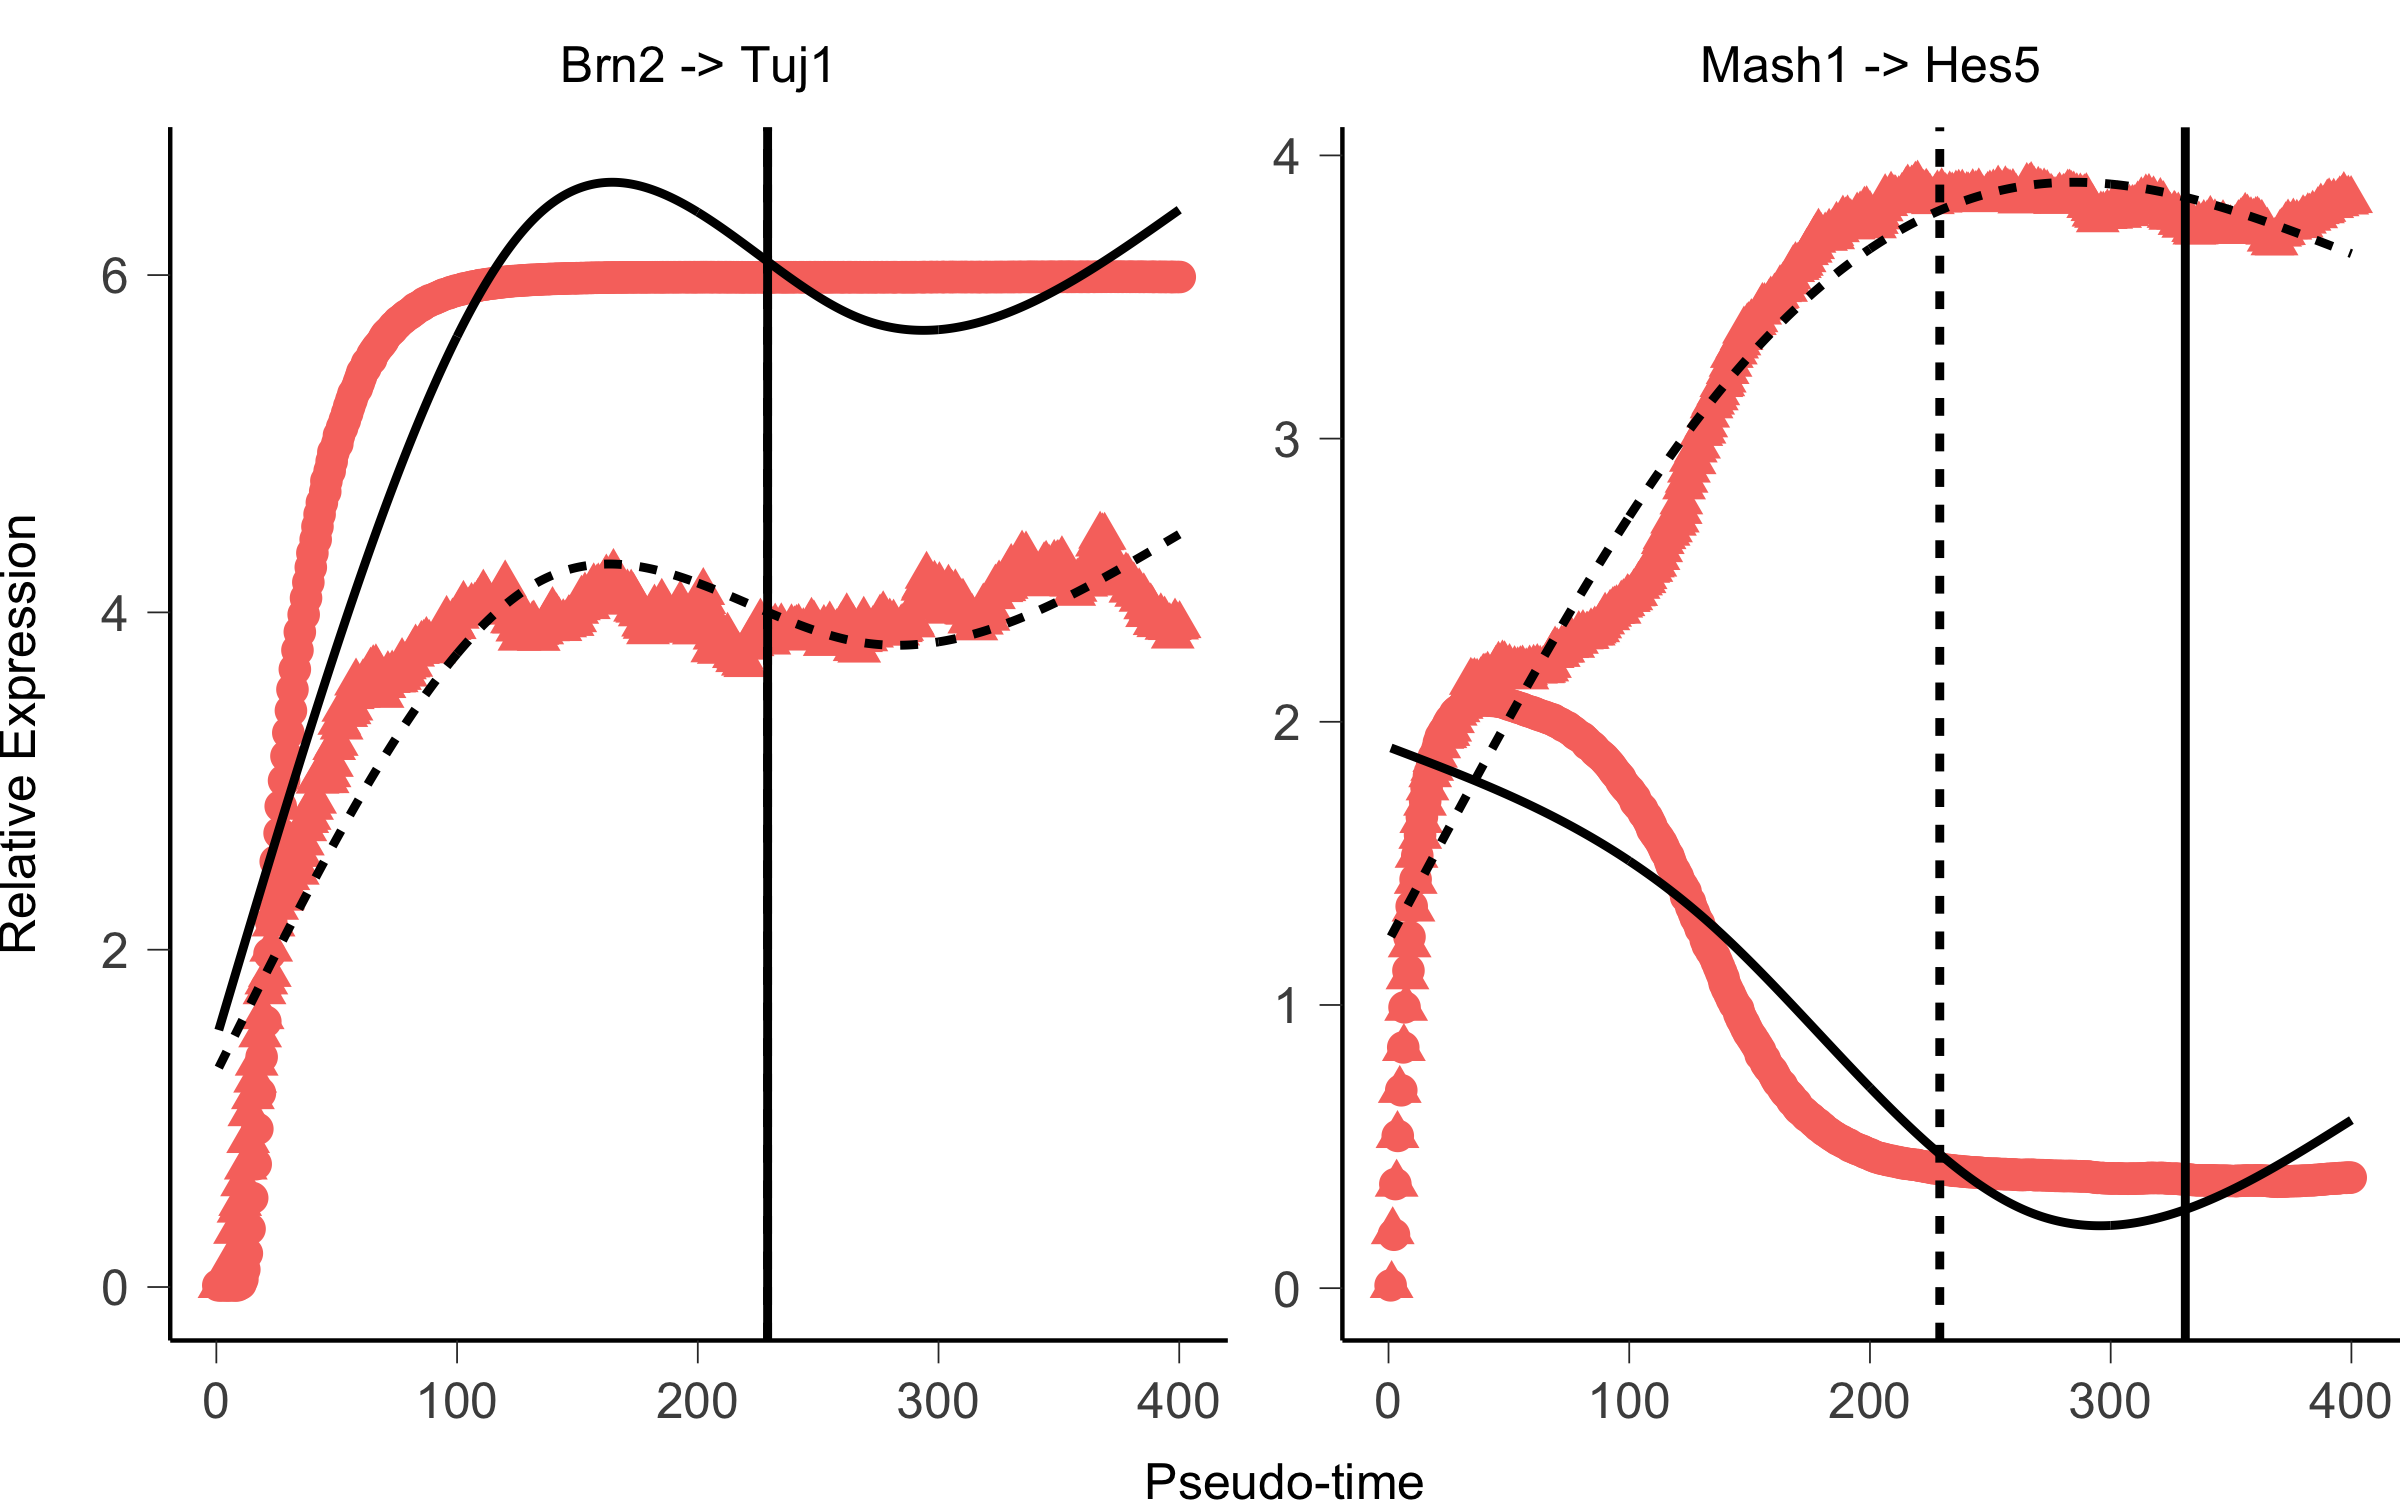
\includegraphics[width=\maxwidth]{figure/gene_pairwise_kinetic_plot-1} 

}


\begin{kframe}\begin{alltt}
\hlkwd{plot_gene_pairs_branched_pseudotime}\hlstd{(na_sim_cds,} \hlkwc{gene_pairs_mat} \hlstd{=} \hlkwd{as.matrix}\hlstd{(neuron_network)[}\hlnum{1}\hlopt{:}\hlnum{2}\hlstd{,} \hlnum{1}\hlopt{:}\hlnum{2}\hlstd{],} \hlkwc{n_row} \hlstd{=} \hlnum{2}\hlstd{,} \hlkwc{n_col} \hlstd{=} \hlnum{2}\hlstd{)} \hlopt{+}
  \hlstd{monocle}\hlopt{:::}\hlkwd{monocle_theme_opts}\hlstd{()} \hlopt{+} \hlstd{xacHelper}\hlopt{::}\hlkwd{nm_theme}\hlstd{()} \hlcom{# neuron_sim_cds is not a branch trajectory }
\end{alltt}
\end{kframe}

{\centering 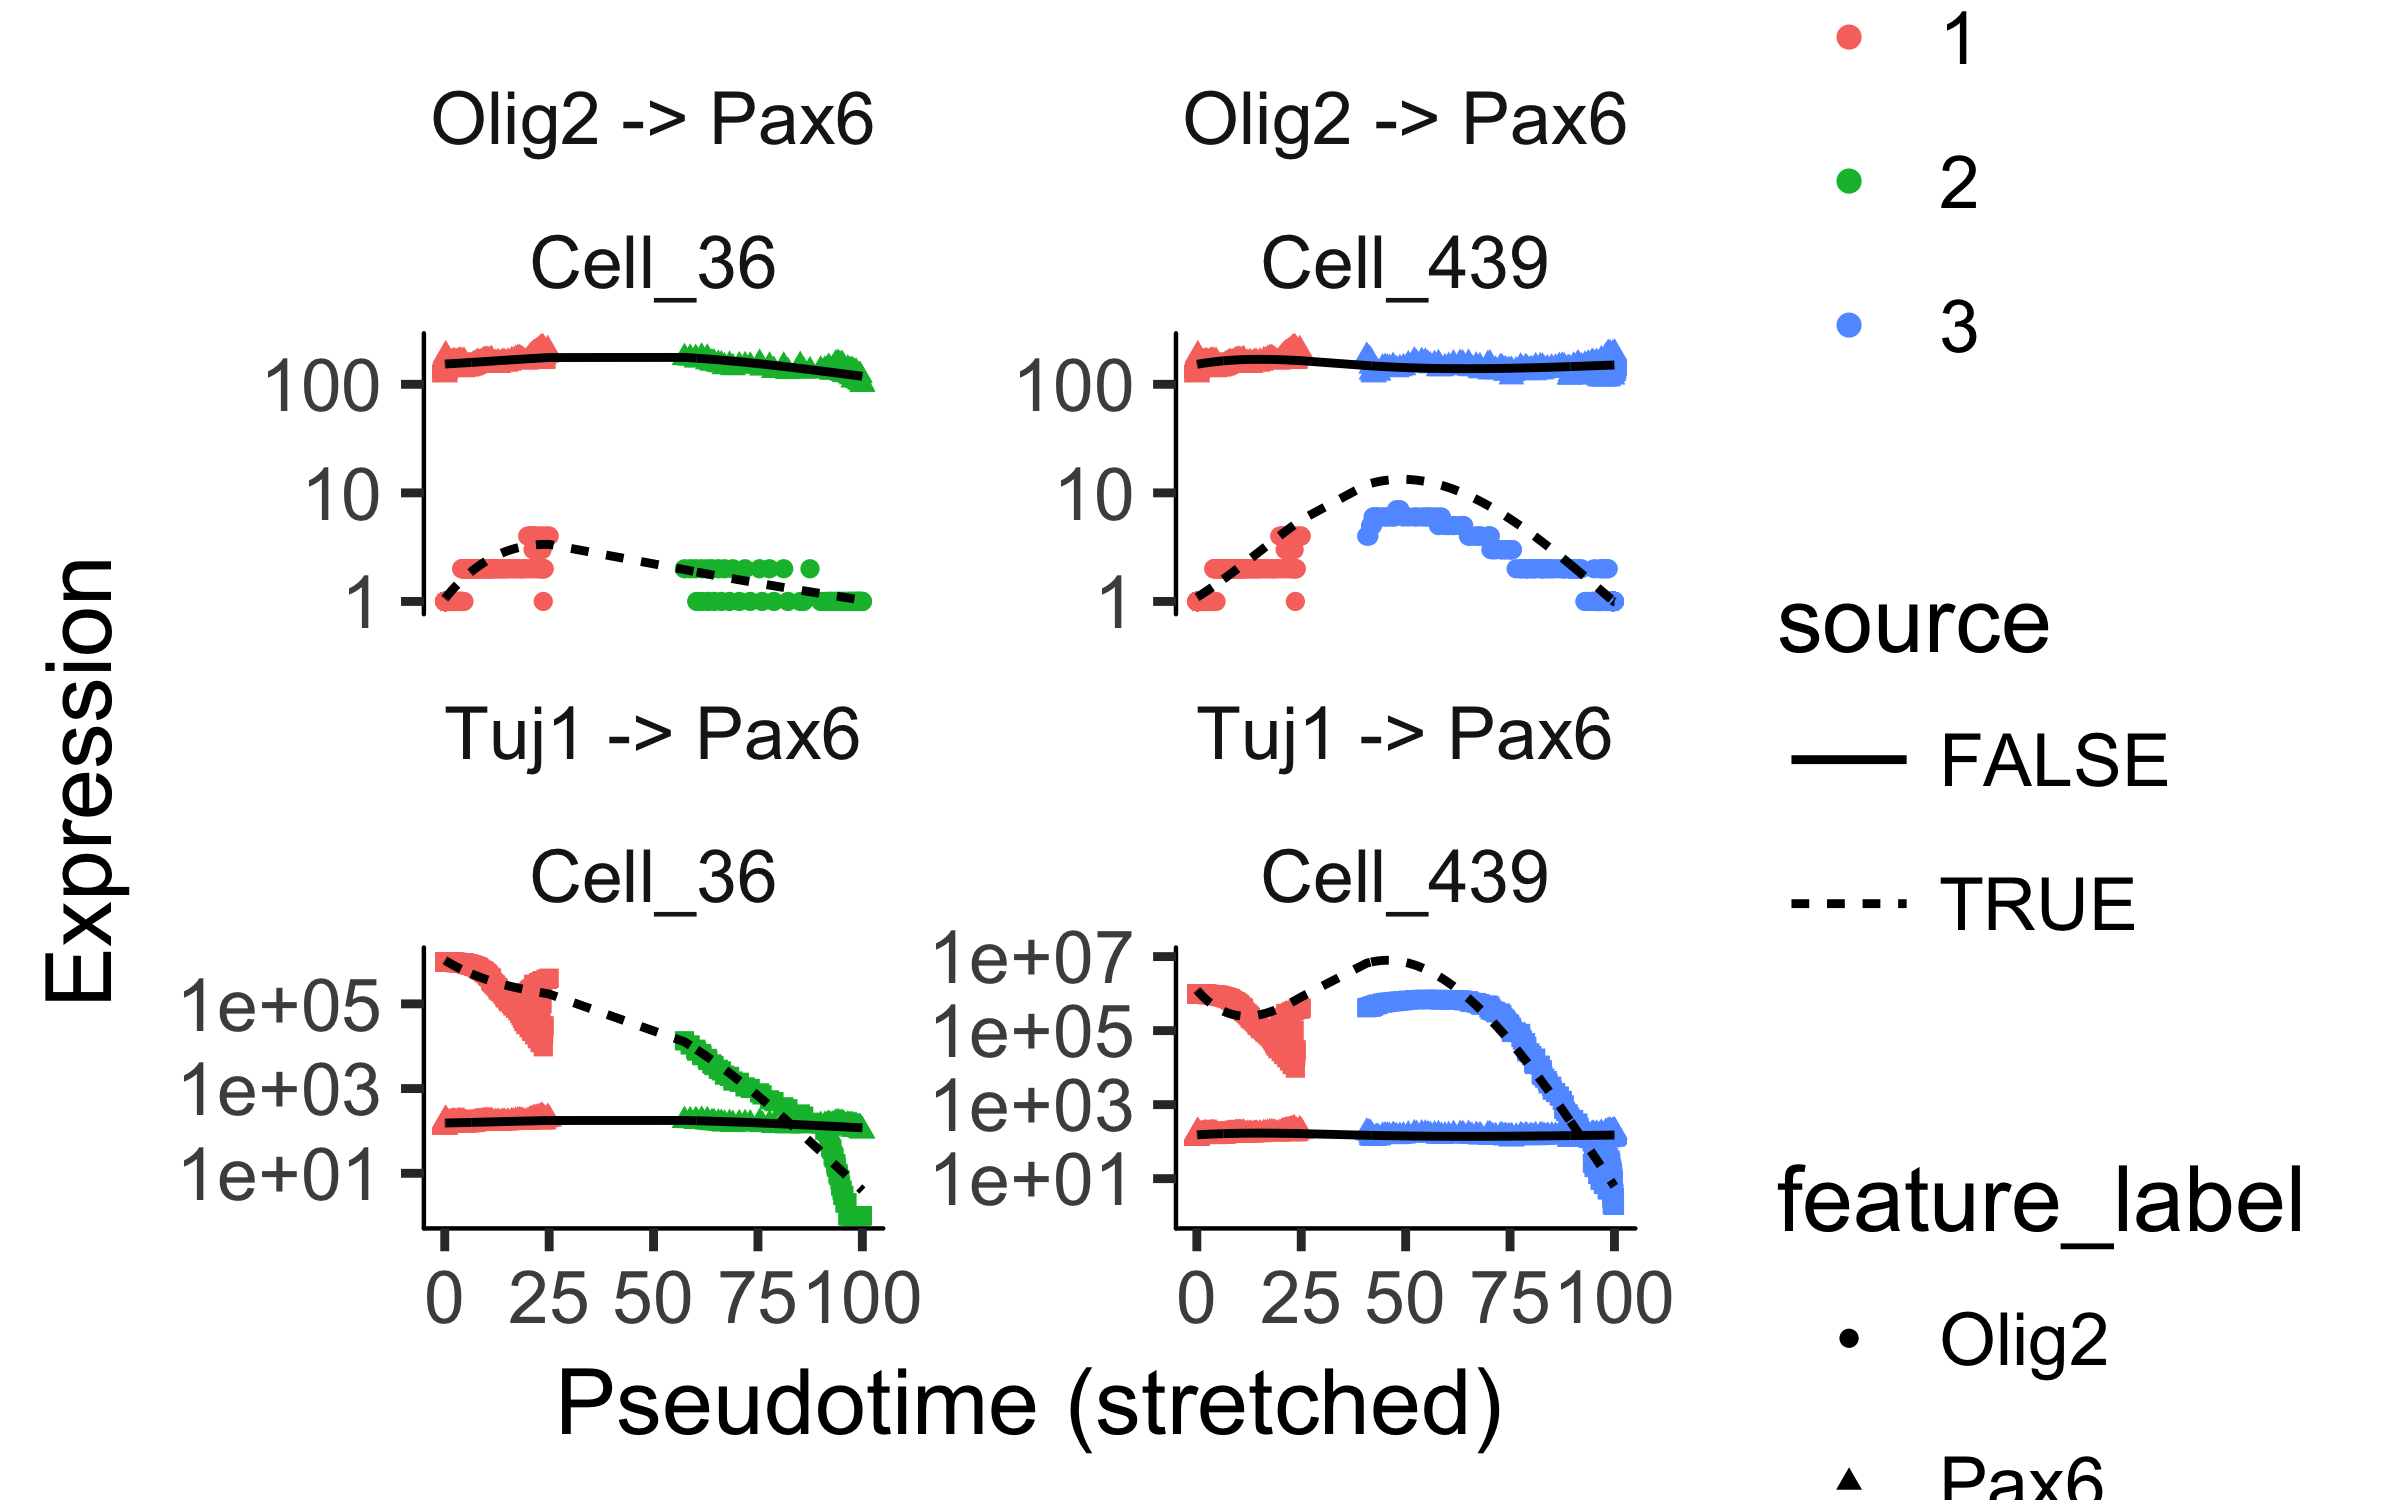
\includegraphics[width=\maxwidth]{figure/gene_pairwise_kinetic_plot-2} 

}



\end{knitrout}

\Rpackage{Scribe} also supports plotting the scatter plot for the gene pair. \textbf{plot\_gene\_pairs} does exactly that but also reveal more abundantly distributed regions with a contour plot. In order to calculate the RDI values, Scribe computes the conditional mutual information of the state for $X_{t - \sigma}$, $Y_t$ and $Y_{t - 1}$ (see methods). We can use \textbf{plot\_rdi\_gene\_pairs} to visualize this state space. An interesting finding from the CCM is that time-lagged data for a single-variable is able to recover a shadow manifold corresponding to the original manifold. Here I will show the 3D space for the variable $Pax6, Mash1, Hes5$ and the shadow manifold for $Y_t, Y_{t - 1}, Y_{t - 2}$ ($Y$ corresponds to $Mash1$). You can immediately identify that the time-lagged shadow manifold captures the topography of the original manifold.

\begin{knitrout}
\definecolor{shadecolor}{rgb}{0.969, 0.969, 0.969}\color{fgcolor}\begin{kframe}
\begin{alltt}
\hlcom{# we skip some functions below because they uses plotly package whose figures can be rendered in a pdf file }
\hlkwd{plot_gene_pairs}\hlstd{(neuron_sim_cds,} \hlkwd{matrix}\hlstd{(}\hlkwd{c}\hlstd{(}\hlstr{'Zic1'}\hlstd{,} \hlstr{'Sox8'}\hlstd{,} \hlstr{'Brn2'}\hlstd{,} \hlstr{'Myt1L'}\hlstd{,} \hlstr{'Tuj1'}\hlstd{,} \hlstr{'Stat3'}\hlstd{),} \hlkwc{ncol} \hlstd{=} \hlnum{2}\hlstd{,} \hlkwc{byrow} \hlstd{= T))} \hlopt{+}
  \hlstd{monocle}\hlopt{:::}\hlkwd{monocle_theme_opts}\hlstd{()} \hlopt{+} \hlstd{xacHelper}\hlopt{::}\hlkwd{nm_theme}\hlstd{()}
\end{alltt}
\end{kframe}

{\centering 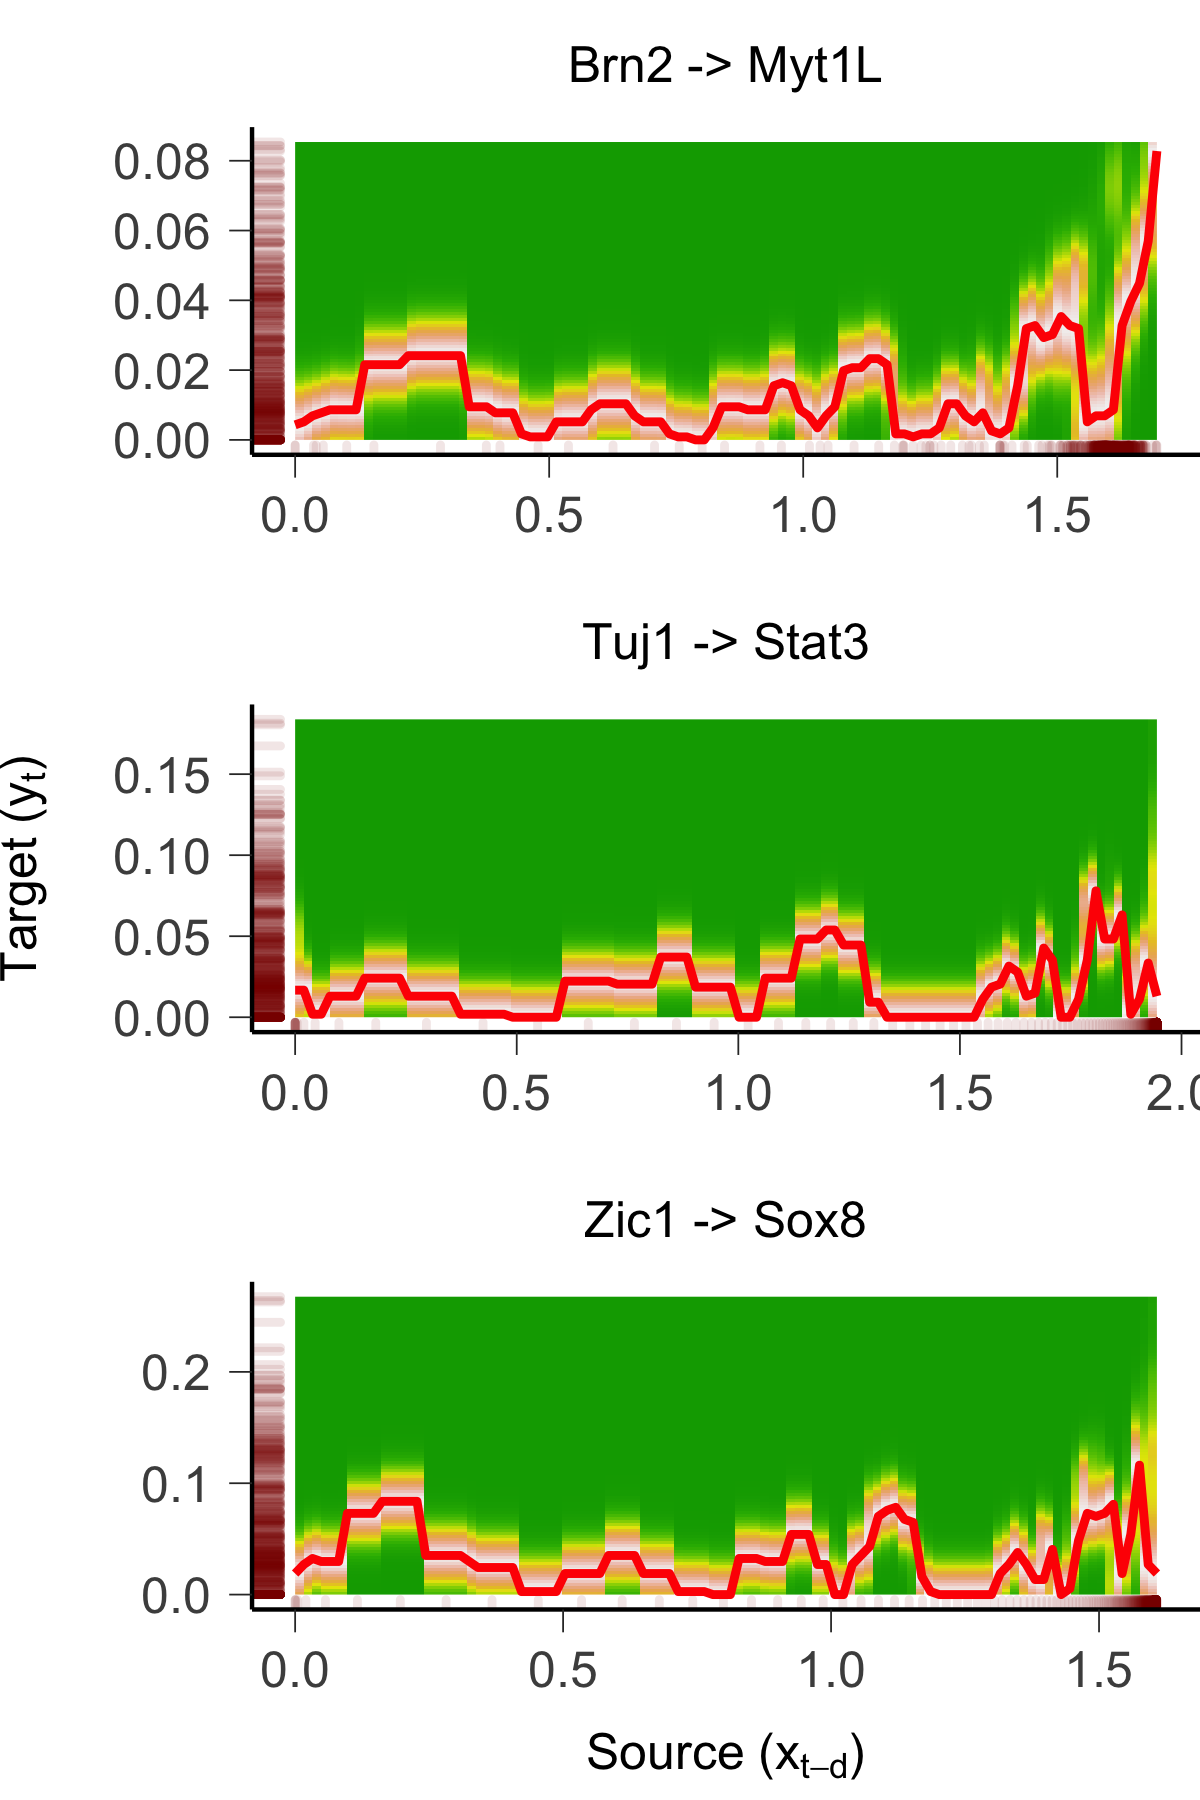
\includegraphics[width=\maxwidth]{figure/gene_pairwise_plot-1} 

}


\begin{kframe}\begin{alltt}
\hlstd{x} \hlkwb{<-} \hlkwd{exprs}\hlstd{(neuron_sim_cds)[}\hlstr{'Pax6'}\hlstd{, ]}
\hlstd{y} \hlkwb{<-} \hlkwd{exprs}\hlstd{(neuron_sim_cds)[}\hlstr{'Mash1'}\hlstd{, ]}
\hlstd{z} \hlkwb{<-} \hlkwd{exprs}\hlstd{(neuron_sim_cds)[}\hlstr{'Hes5'}\hlstd{, ]}

\hlcom{# plot_rdi_gene_pairs(x, y)}

\hlcom{# plot_ly(type = 'scatter3d', x = log10(x), y = log10(y), z = log10(z), mode = 'markers') # show the original space}
\hlcom{# }
\hlcom{# # plot CCM state space and the the scatter plot in three dimension}
\hlcom{# plot_ccm(x) # Pax lagged state space looks pretty random}
\hlcom{# }
\hlcom{# plot_ccm(log10(y)) #Pax lagged state space looks pretty random}
\hlcom{# }
\hlcom{# plot_ccm(z) #Pax lagged state space looks pretty random}
\end{alltt}
\end{kframe}
\end{knitrout}

In order to intuitively visualize the relationship between two genes, we extend the DREVI approach, originally proposed by Smita Krishnaswamy, et. al. In the original approach, DREVI doesn't consider time delay, the \textbf{plot\_rdi\_pairs} function in \Rpackage{Scribe} can be used to visualize both the original \Rpackage{DREVI} method as well as time-delayed \Rpackage{DREVI} results. From the positive and negative gene pairs, we can see the response curve for the interacting gene pairs are pretty smooth while the non-interacting genes looks pretty noisy and less smooth. Moreover, from the \Rpackage{DREVI} plot for the non-interacting gene pair, a give target value can have many more corresponding source values and that the response curve is pretty much flat.

Moreover, in order to better represent the RDI values, we also implemented a generalized approach to consider the effect of $Y$ at earlier time point. We achieve this first by fitting a curve between $Y_t, Y_{t - 1}$ and then obtain the residual for this fitting. We then plot these residual and $X_{t - \sigma}$ time-delayed DREVI to visualize the gene regulation.

\begin{knitrout}
\definecolor{shadecolor}{rgb}{0.969, 0.969, 0.969}\color{fgcolor}\begin{kframe}
\begin{alltt}
\hlcom{# show the drevi plot result for all existing edges:}
\hlkwd{plot_rdi_pairs}\hlstd{(neuron_sim_cds[,} \hlnum{1}\hlopt{:}\hlnum{200}\hlstd{],} \hlkwc{gene_pairs_mat} \hlstd{=} \hlkwd{as.matrix}\hlstd{(neuron_network[}\hlkwd{c}\hlstd{(}\hlnum{1}\hlstd{,} \hlnum{3}\hlstd{),} \hlnum{1}\hlopt{:}\hlnum{2}\hlstd{]),} \hlkwc{d} \hlstd{=} \hlnum{1}\hlstd{,} \hlkwc{n_row} \hlstd{=} \hlnum{1}\hlstd{,} \hlkwc{n_col} \hlstd{=} \hlnum{2}\hlstd{)} \hlopt{+}
  \hlstd{monocle}\hlopt{:::}\hlkwd{monocle_theme_opts}\hlstd{()} \hlopt{+} \hlstd{xacHelper}\hlopt{::}\hlkwd{nm_theme}\hlstd{()}
\end{alltt}
\end{kframe}

{\centering 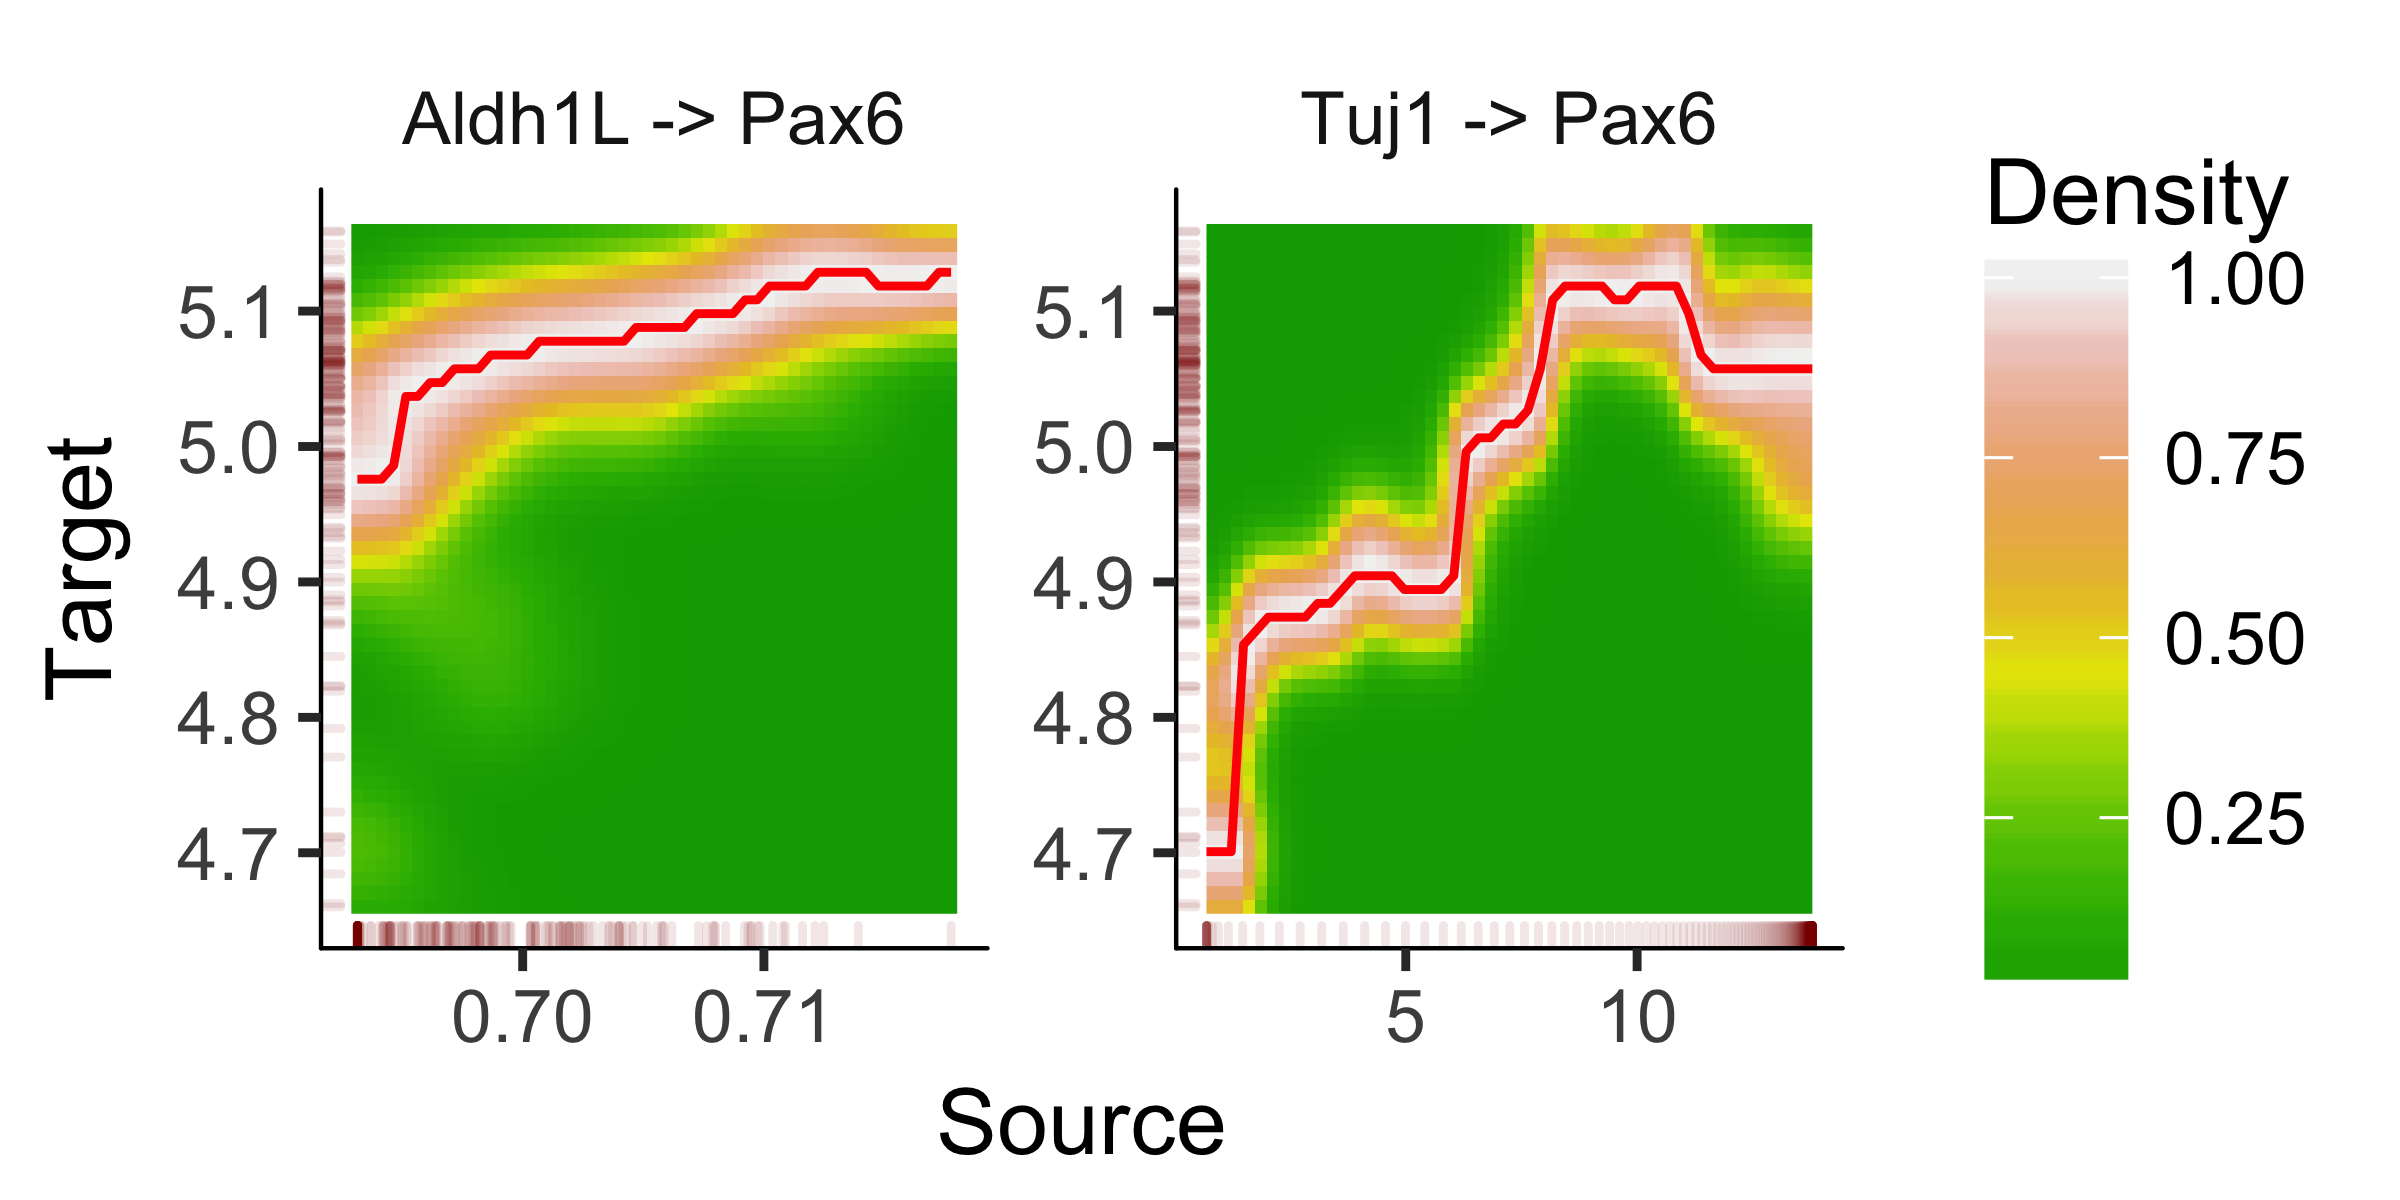
\includegraphics[width=\maxwidth]{figure/plot_drevi-1} 

}


\begin{kframe}\begin{alltt}
\hlkwd{plot_rdi_pairs}\hlstd{(neuron_sim_cds[,} \hlnum{1}\hlopt{:}\hlnum{200}\hlstd{],} \hlkwc{gene_pairs_mat} \hlstd{=} \hlkwd{matrix}\hlstd{(}\hlkwd{c}\hlstd{(}\hlstr{'Zic1'}\hlstd{,} \hlstr{'Sox8'}\hlstd{,} \hlstr{'Brn2'}\hlstd{,} \hlstr{'Myt1L'}\hlstd{),} \hlkwc{byrow} \hlstd{= T,} \hlkwc{nrow} \hlstd{=} \hlnum{2}\hlstd{),} \hlkwc{n_row} \hlstd{=} \hlnum{1}\hlstd{,} \hlkwc{n_col} \hlstd{=} \hlnum{2}\hlstd{,} \hlkwc{scales} \hlstd{=} \hlstr{'free'}\hlstd{)} \hlopt{+}
  \hlstd{monocle}\hlopt{:::}\hlkwd{monocle_theme_opts}\hlstd{()} \hlopt{+} \hlstd{xacHelper}\hlopt{::}\hlkwd{nm_theme}\hlstd{()}
\end{alltt}
\end{kframe}

{\centering 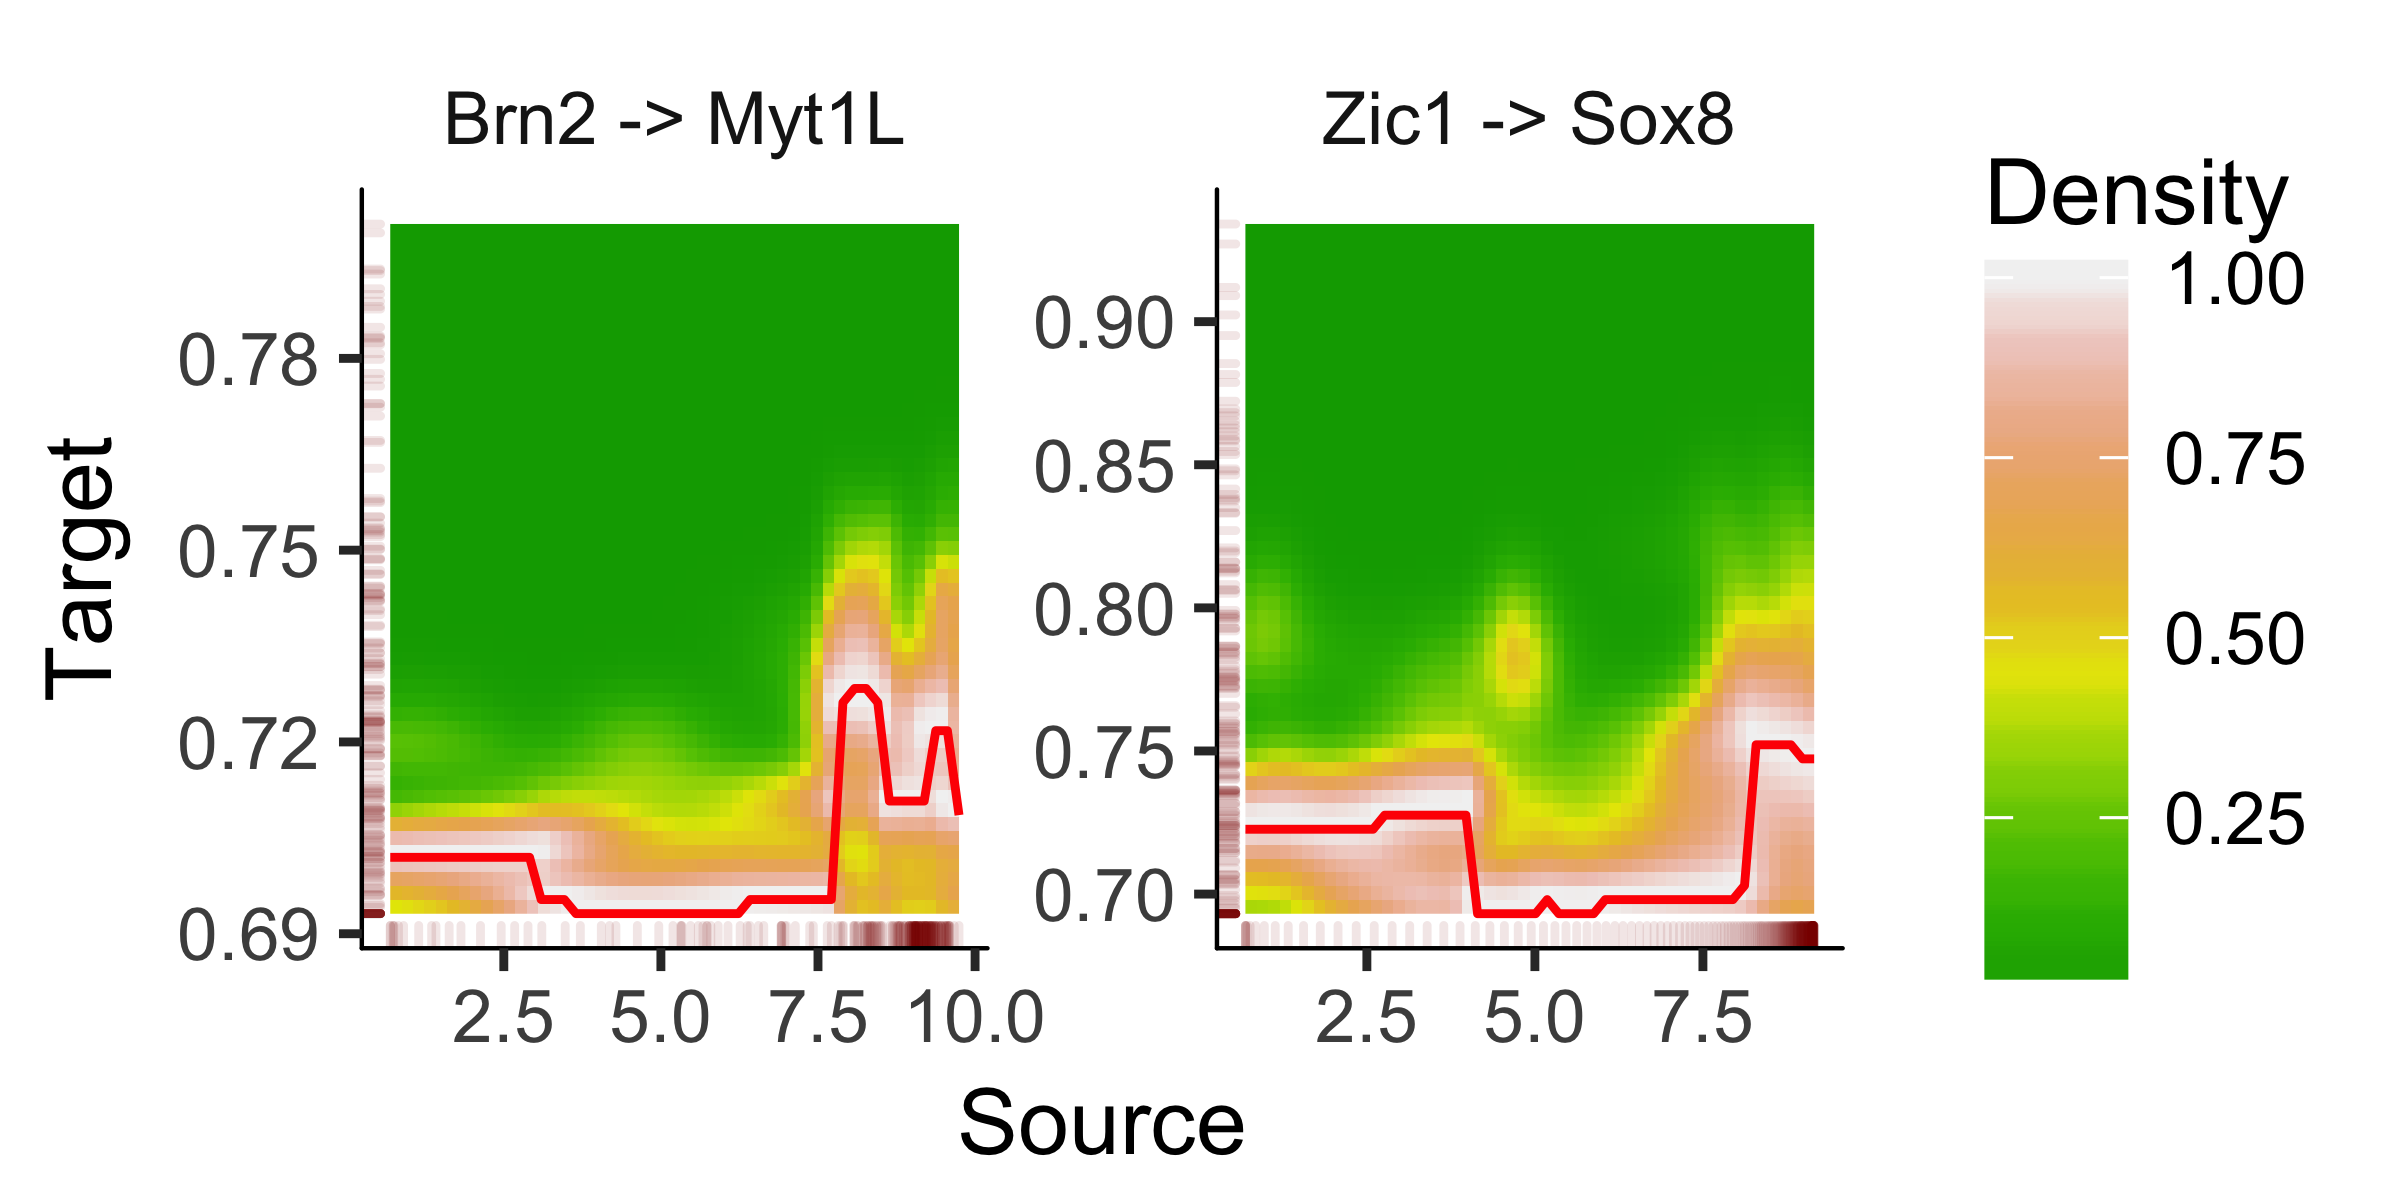
\includegraphics[width=\maxwidth]{figure/plot_drevi-2} 

}



\end{knitrout}

\subsection{Assess temporal causal gene regulation}

Gene regulation is dynamic and the timing of regulation varies from gene-pair to gene-pair. We developed a strategy (implemented through the \textbf{rdi\_crdi\_pseudotime} function) to estimate the temporal causal regulation in \Rpackage{Scribe} to helps to identify the period of strong gene regulation.
\begin{knitrout}
\definecolor{shadecolor}{rgb}{0.969, 0.969, 0.969}\color{fgcolor}\begin{kframe}
\begin{alltt}
\hlcom{# test temporal RDI, etc.}
\hlstd{gene_name_vec} \hlkwb{<-} \hlkwd{c}\hlstd{(}\hlstr{'Pax6'}\hlstd{,} \hlstr{'Mash1'}\hlstd{,} \hlstr{'Brn2'}\hlstd{,} \hlstr{'Zic1'}\hlstd{,} \hlstr{'Tuj1'}\hlstd{,} \hlstr{'Hes5'}\hlstd{,} \hlstr{'Scl'}\hlstd{,} \hlstr{'Olig2'}\hlstd{,} \hlstr{'Stat3'}\hlstd{,} \hlstr{'Myt1L'}\hlstd{,} \hlstr{'Aldh1L'}\hlstd{,} \hlstr{'Sox8'}\hlstd{,} \hlstr{'Mature'}\hlstd{)}

\hlstd{rdi_crdi_pseudotime_res_list} \hlkwb{<-} \hlkwd{rdi_crdi_pseudotime}\hlstd{(}\hlkwd{t}\hlstd{(}\hlkwd{exprs}\hlstd{(na_sim_cds)[}\hlnum{1}\hlopt{:}\hlnum{12}\hlstd{,} \hlnum{1}\hlopt{:}\hlnum{200}\hlstd{]),} \hlkwc{window_size} \hlstd{=} \hlnum{50}\hlstd{)} \hlcom{#13 mature gives Na values}

\hlstd{rdi_res} \hlkwb{<-} \hlstd{rdi_crdi_pseudotime_res_list}\hlopt{$}\hlstd{rdi_res}
\hlstd{crdi_res} \hlkwb{<-} \hlstd{rdi_crdi_pseudotime_res_list}\hlopt{$}\hlstd{crdi_res}

\hlkwd{dim}\hlstd{(rdi_res)} \hlkwb{<-} \hlkwd{c}\hlstd{(}\hlkwd{dim}\hlstd{(rdi_res)[}\hlnum{1}\hlstd{],} \hlkwd{dim}\hlstd{(rdi_res)[}\hlnum{2}\hlstd{]} \hlopt{*} \hlkwd{dim}\hlstd{(rdi_res)[}\hlnum{2}\hlstd{])}

\hlstd{all_cmbns} \hlkwb{<-} \hlkwd{expand.grid}\hlstd{(gene_name_vec[}\hlnum{1}\hlopt{:}\hlnum{12}\hlstd{], gene_name_vec[}\hlnum{1}\hlopt{:}\hlnum{12}\hlstd{])}
\hlstd{valid_all_cmbns_df} \hlkwb{<-} \hlkwd{data.frame}\hlstd{(}\hlkwc{pair} \hlstd{=} \hlkwd{paste}\hlstd{((all_cmbns}\hlopt{$}\hlstd{Var1), (all_cmbns}\hlopt{$}\hlstd{Var2),} \hlkwc{sep} \hlstd{=} \hlstr{' -> '}\hlstd{),} \hlkwc{pval} \hlstd{=} \hlnum{0}\hlstd{)}

\hlkwd{row.names}\hlstd{(valid_all_cmbns_df)} \hlkwb{<-} \hlstd{valid_all_cmbns_df}\hlopt{$}\hlstd{pair}
\hlstd{rdi_res} \hlkwb{<-} \hlkwd{as.data.frame}\hlstd{(rdi_res)}
\hlkwd{colnames}\hlstd{(rdi_res)} \hlkwb{<-} \hlstd{valid_all_cmbns_df}\hlopt{$}\hlstd{pair}

\hlstd{valid_all_cmbns_df} \hlkwb{<-} \hlkwd{data.frame}\hlstd{(}\hlkwc{pair} \hlstd{=} \hlkwd{paste}\hlstd{((}\hlkwd{as.character}\hlstd{(neuron_network[,} \hlnum{1}\hlstd{])), (}\hlkwd{as.character}\hlstd{(neuron_network[,} \hlnum{2}\hlstd{])),} \hlkwc{sep} \hlstd{=} \hlstr{' -> '}\hlstd{),} \hlkwc{pval} \hlstd{=} \hlnum{0}\hlstd{)}
\hlstd{valid_rdi_res} \hlkwb{<-} \hlstd{rdi_res[,} \hlkwd{as.character}\hlstd{(valid_all_cmbns_df}\hlopt{$}\hlstd{pair)]}
\hlstd{norm_valid_rdi_res} \hlkwb{<-} \hlkwd{apply}\hlstd{(valid_rdi_res,} \hlnum{2}\hlstd{,} \hlkwa{function}\hlstd{(}\hlkwc{x}\hlstd{) (x} \hlopt{-} \hlkwd{min}\hlstd{(x))} \hlopt{/} \hlstd{(}\hlkwd{max}\hlstd{(x)} \hlopt{-} \hlkwd{min}\hlstd{(x)))}
\hlstd{pheatmap}\hlopt{::}\hlkwd{pheatmap}\hlstd{(}\hlkwd{t}\hlstd{(norm_valid_rdi_res[, ]),} \hlkwc{cluster_rows} \hlstd{= F,} \hlkwc{cluster_cols} \hlstd{= F,} \hlkwc{annotation_names_row} \hlstd{= T,} \hlkwc{border_color} \hlstd{=} \hlnum{NA}\hlstd{)}
\end{alltt}
\end{kframe}

{\centering 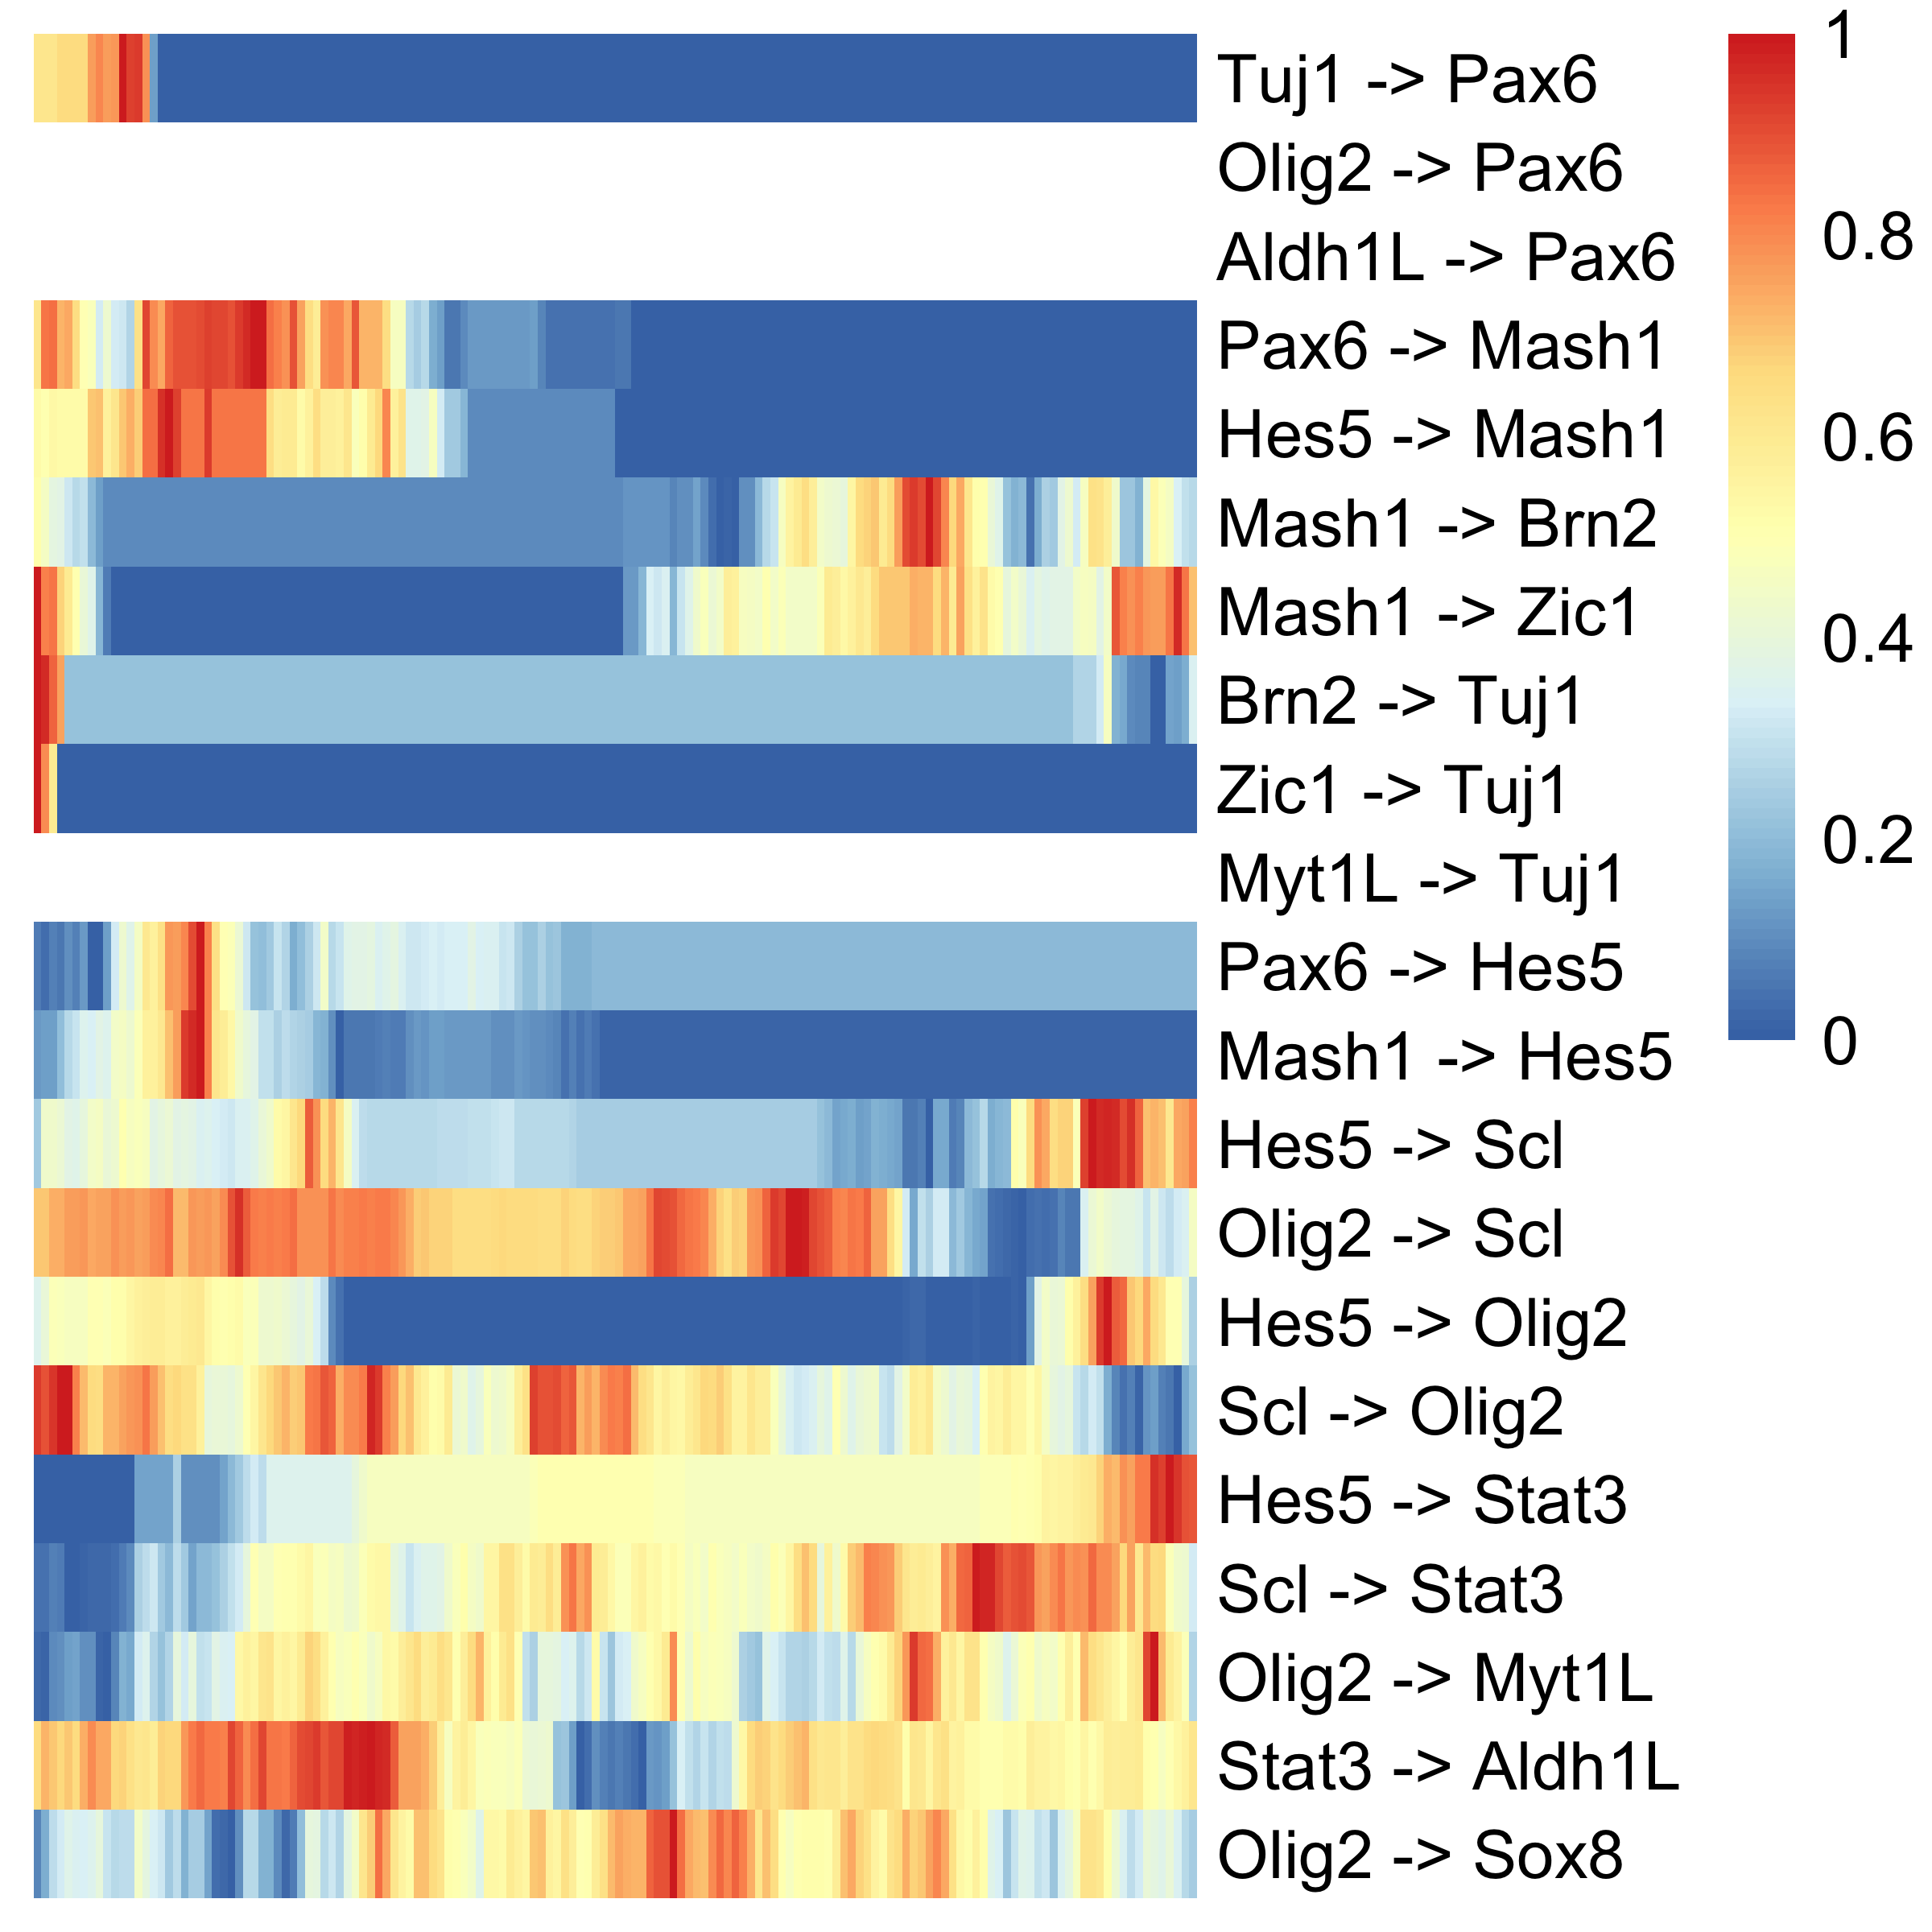
\includegraphics[width=\maxwidth]{figure/plot_temporal_rdi-1} 

}


\begin{kframe}\begin{alltt}
\hlstd{valid_all_cmbns_df_back} \hlkwb{<-} \hlkwd{data.frame}\hlstd{(}\hlkwc{pair} \hlstd{=} \hlkwd{paste}\hlstd{((}\hlkwd{as.character}\hlstd{(neuron_network[,} \hlnum{1}\hlstd{])), (}\hlkwd{as.character}\hlstd{(neuron_network[,} \hlnum{2}\hlstd{])),} \hlkwc{sep} \hlstd{=} \hlstr{' -> '}\hlstd{),} \hlkwc{pval} \hlstd{=} \hlnum{0}\hlstd{)}
\hlstd{valid_rdi_res_back} \hlkwb{<-} \hlstd{rdi_res[,} \hlkwd{as.character}\hlstd{(valid_all_cmbns_df_back}\hlopt{$}\hlstd{pair)]}
\hlstd{norm_valid_rdi_res_back} \hlkwb{<-} \hlkwd{apply}\hlstd{(valid_rdi_res_back,} \hlnum{2}\hlstd{,} \hlkwa{function}\hlstd{(}\hlkwc{x}\hlstd{) (x} \hlopt{-} \hlkwd{min}\hlstd{(x))} \hlopt{/} \hlstd{(}\hlkwd{max}\hlstd{(x)} \hlopt{-} \hlkwd{min}\hlstd{(x)))}
\hlstd{pheatmap}\hlopt{::}\hlkwd{pheatmap}\hlstd{(}\hlkwd{t}\hlstd{(norm_valid_rdi_res_back[, ]),} \hlkwc{cluster_rows} \hlstd{= F,} \hlkwc{cluster_cols} \hlstd{= F,} \hlkwc{annotation_names_row} \hlstd{= T,} \hlkwc{border_color} \hlstd{=} \hlnum{NA}\hlstd{)}
\end{alltt}
\end{kframe}

{\centering 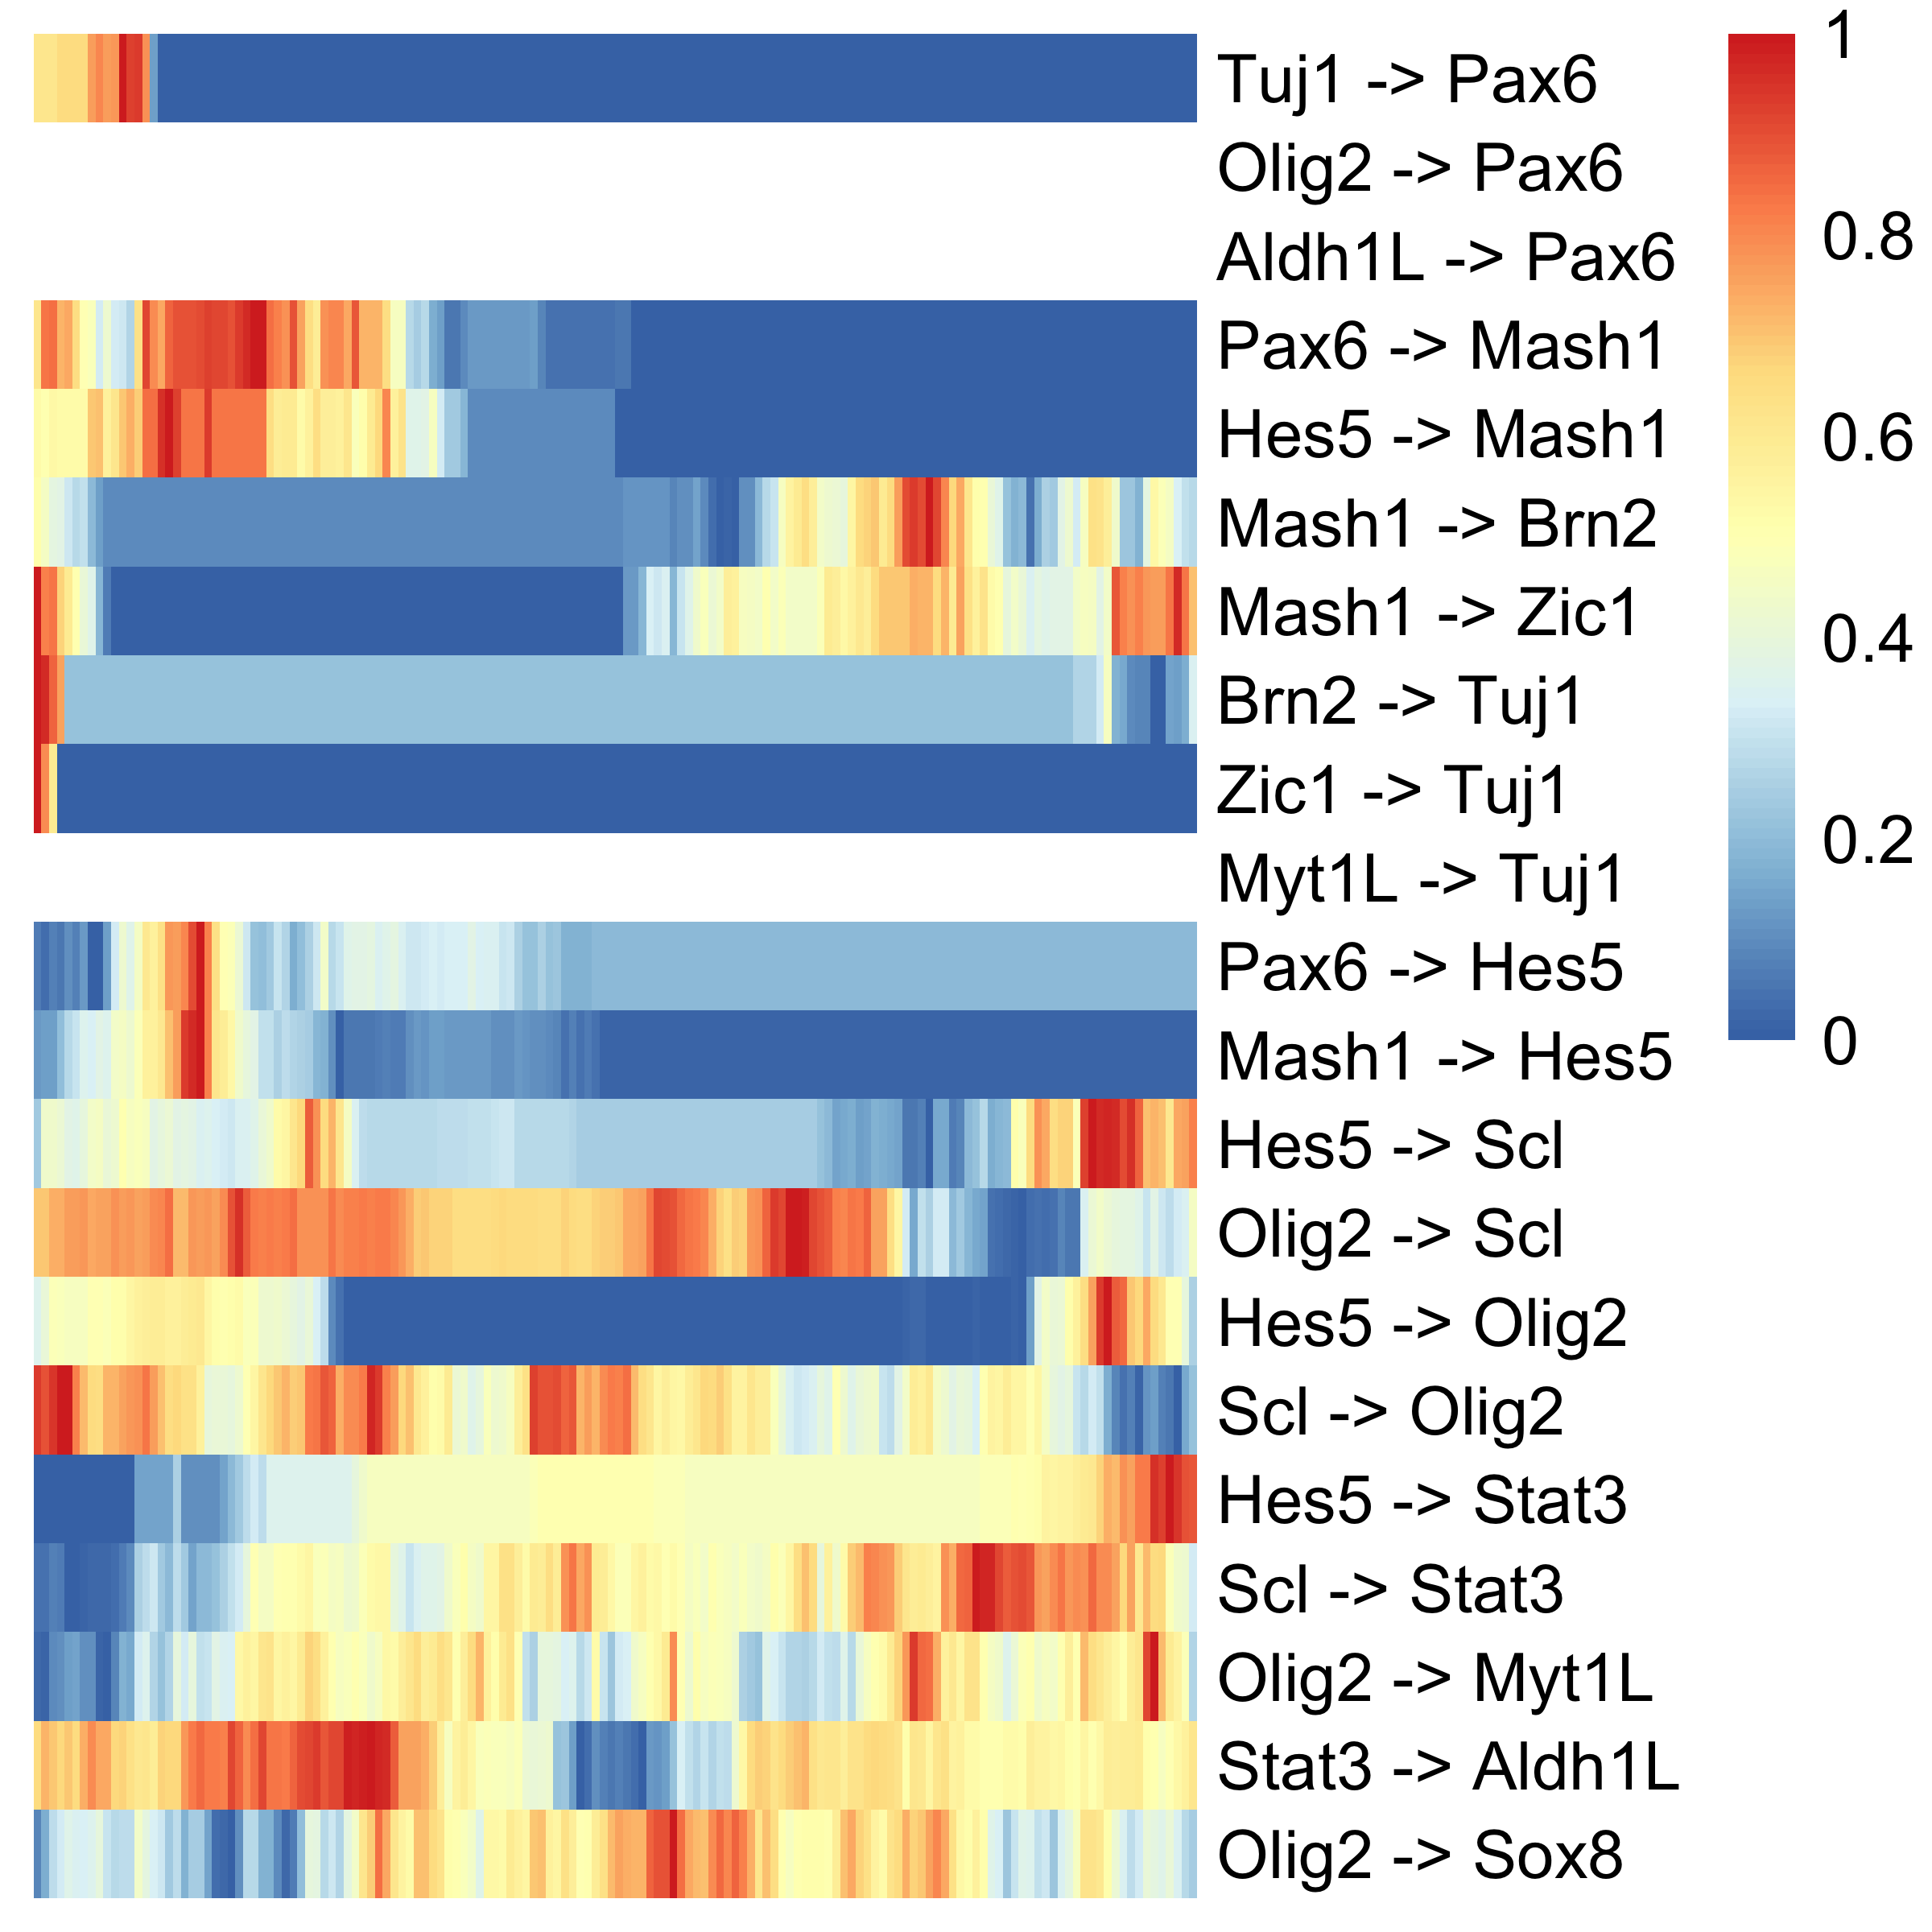
\includegraphics[width=\maxwidth]{figure/plot_temporal_rdi-2} 

}


\begin{kframe}\begin{alltt}
\hlcom{# plot crdi_res}
\hlkwd{dim}\hlstd{(crdi_res)} \hlkwb{<-} \hlkwd{c}\hlstd{(}\hlkwd{dim}\hlstd{(crdi_res)[}\hlnum{1}\hlstd{],} \hlkwd{dim}\hlstd{(crdi_res)[}\hlnum{2}\hlstd{]} \hlopt{*} \hlkwd{dim}\hlstd{(crdi_res)[}\hlnum{2}\hlstd{])}

\hlstd{valid_all_cmbns_df} \hlkwb{<-} \hlkwd{data.frame}\hlstd{(}\hlkwc{pair} \hlstd{=} \hlkwd{paste}\hlstd{((all_cmbns}\hlopt{$}\hlstd{Var1), (all_cmbns}\hlopt{$}\hlstd{Var2),} \hlkwc{sep} \hlstd{=} \hlstr{' -> '}\hlstd{),} \hlkwc{pval} \hlstd{=} \hlnum{0}\hlstd{)}
\hlkwd{colnames}\hlstd{(crdi_res)} \hlkwb{<-} \hlstd{valid_all_cmbns_df}\hlopt{$}\hlstd{pair}

\hlstd{valid_all_cmbns_df} \hlkwb{<-} \hlkwd{data.frame}\hlstd{(}\hlkwc{pair} \hlstd{=} \hlkwd{paste}\hlstd{((}\hlkwd{as.character}\hlstd{(neuron_network[,} \hlnum{1}\hlstd{])), (}\hlkwd{as.character}\hlstd{(neuron_network[,} \hlnum{2}\hlstd{])),} \hlkwc{sep} \hlstd{=} \hlstr{' -> '}\hlstd{),} \hlkwc{pval} \hlstd{=} \hlnum{0}\hlstd{)}
\hlstd{valid_crdi_res} \hlkwb{<-} \hlstd{crdi_res[,} \hlkwd{as.character}\hlstd{(valid_all_cmbns_df}\hlopt{$}\hlstd{pair)]}
\hlstd{norm_valid_crdi_res} \hlkwb{<-} \hlkwd{apply}\hlstd{(valid_crdi_res,} \hlnum{2}\hlstd{,} \hlkwa{function}\hlstd{(}\hlkwc{x}\hlstd{) (x} \hlopt{-} \hlkwd{min}\hlstd{(x))} \hlopt{/} \hlstd{(}\hlkwd{max}\hlstd{(x)} \hlopt{-} \hlkwd{min}\hlstd{(x)))}
\hlcom{# norm_valid_crdi_res_ordered <- norm_valid_crdi_res[, order(unlist(apply(norm_valid_crdi_res, 2, which.max)))]}
\hlstd{pheatmap}\hlopt{::}\hlkwd{pheatmap}\hlstd{(}\hlkwd{t}\hlstd{(norm_valid_crdi_res[, ]),} \hlkwc{cluster_rows} \hlstd{= F,} \hlkwc{cluster_cols} \hlstd{= F,} \hlkwc{annotation_names_row} \hlstd{= T,} \hlkwc{border_color} \hlstd{=} \hlnum{NA}\hlstd{)}
\end{alltt}
\end{kframe}

{\centering 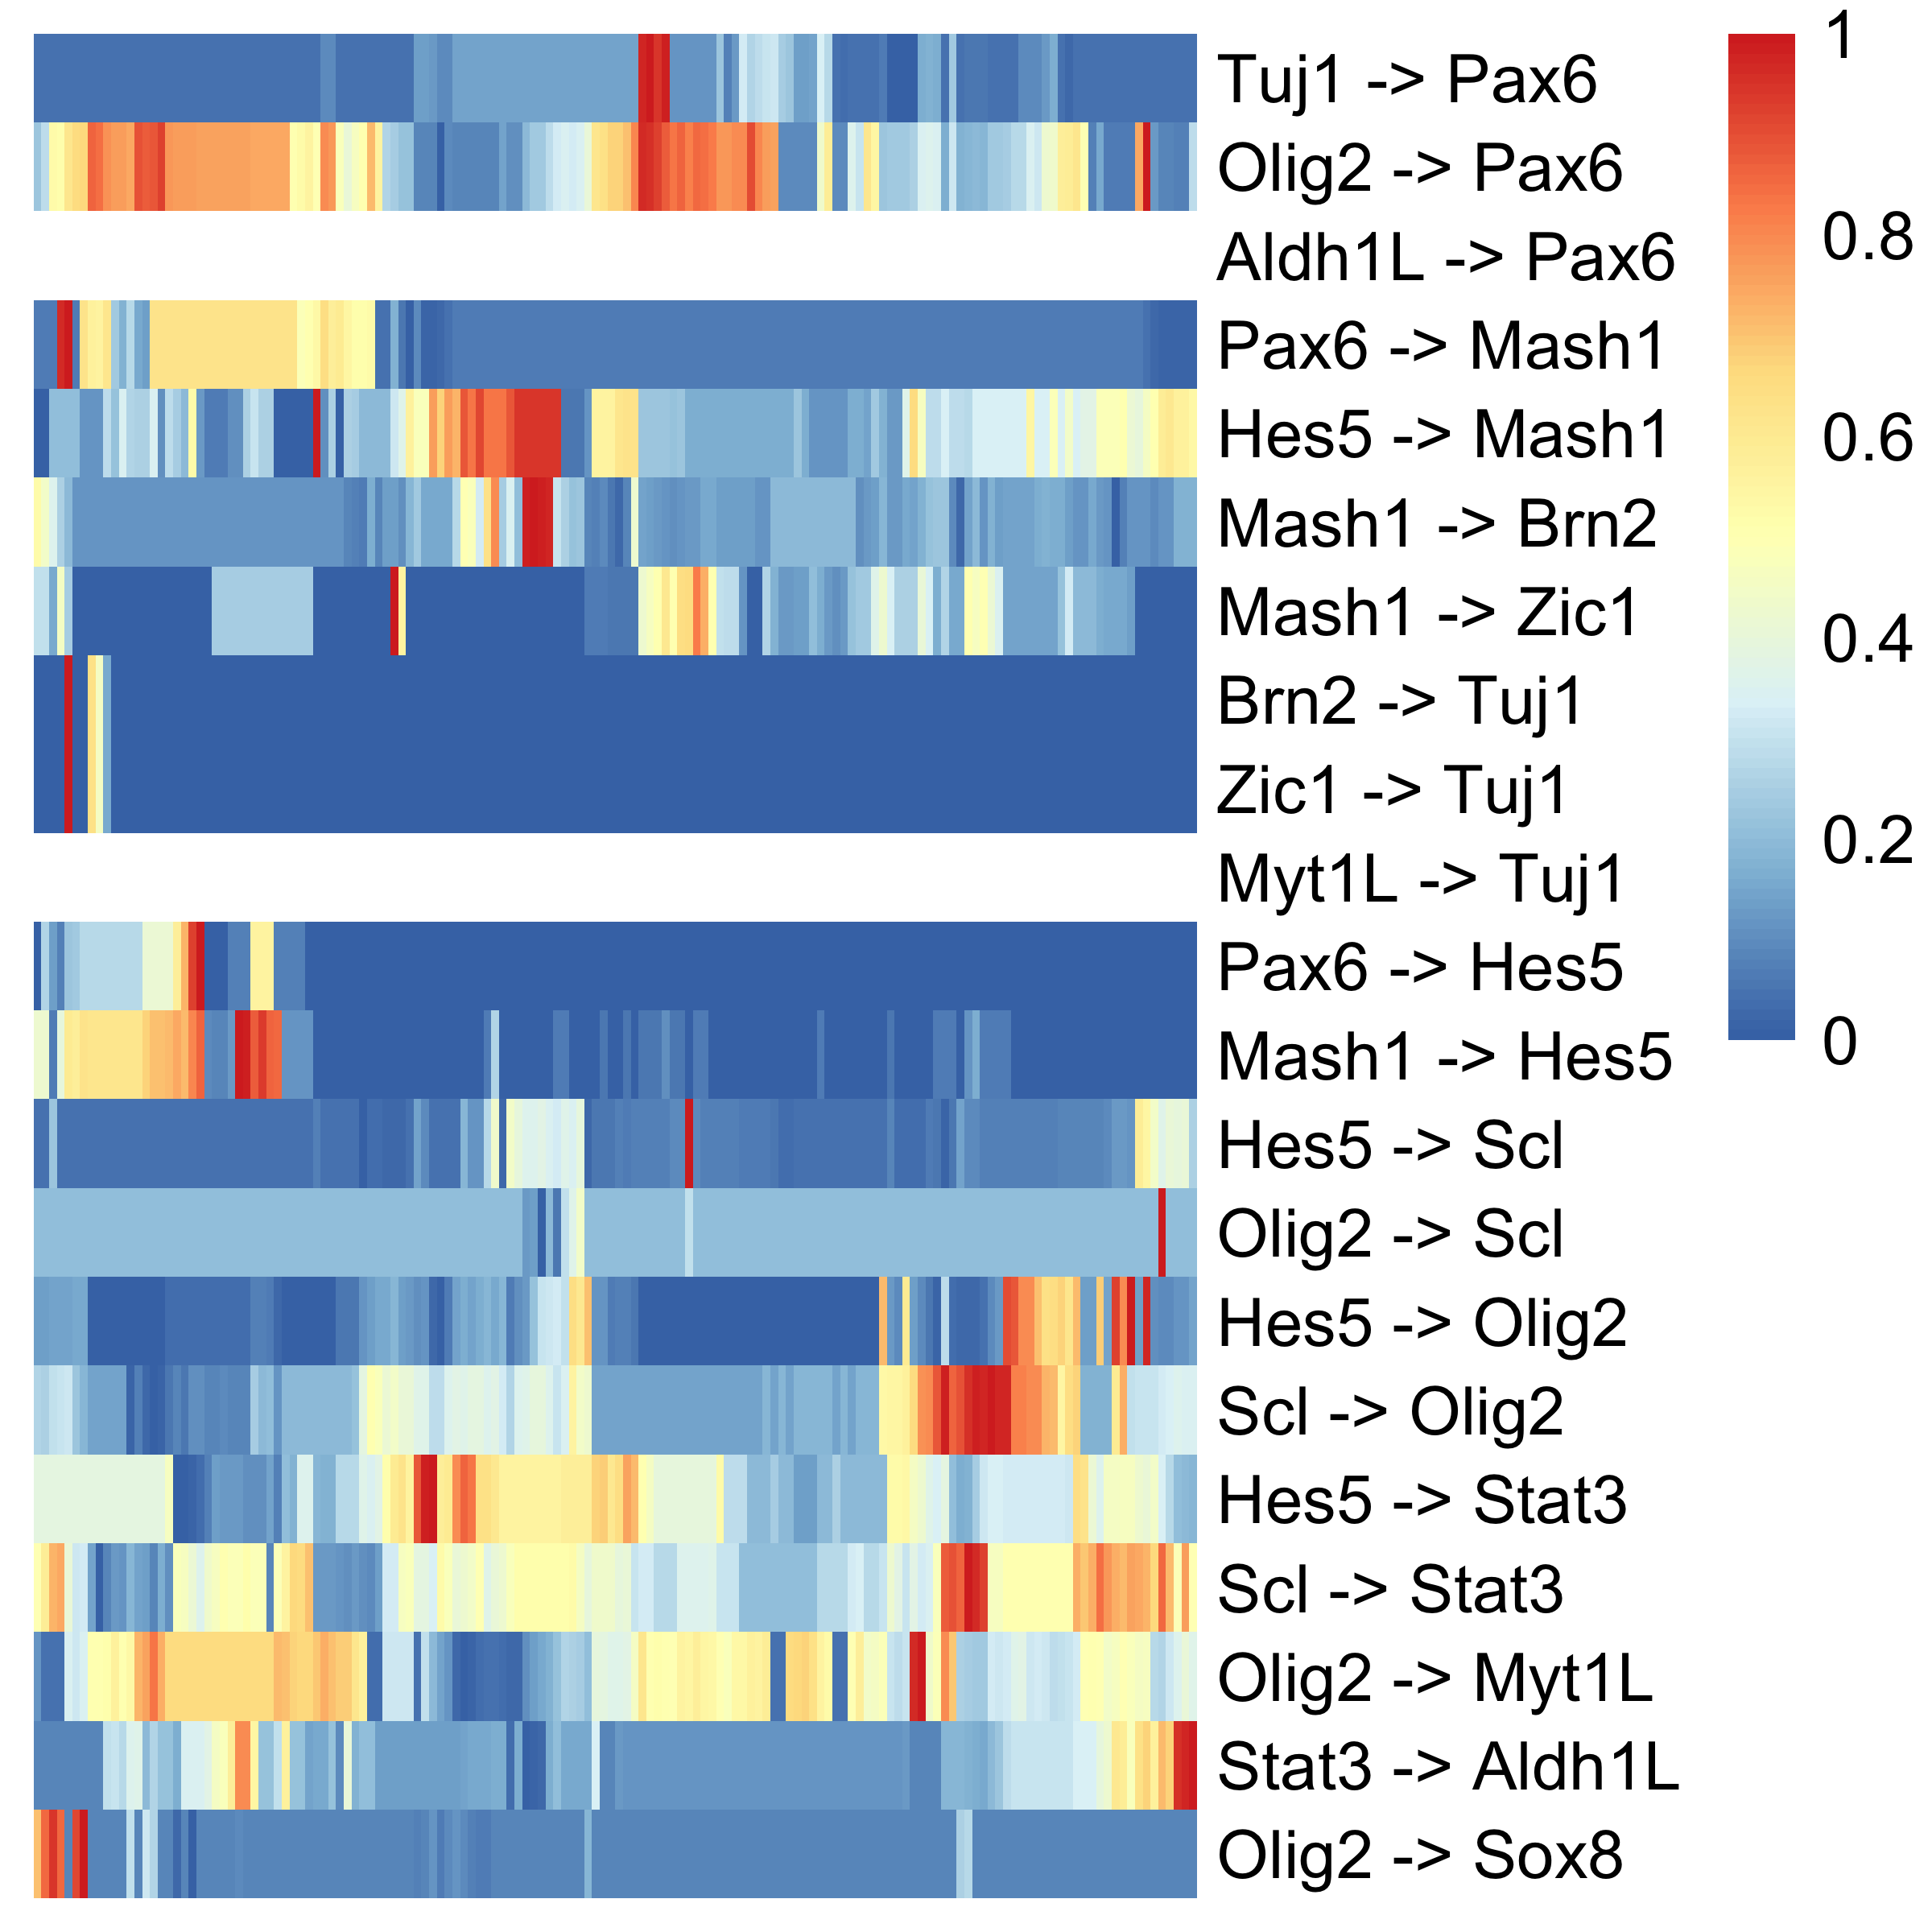
\includegraphics[width=\maxwidth]{figure/plot_temporal_rdi-3} 

}


\begin{kframe}\begin{alltt}
\hlstd{pheatmap}\hlopt{::}\hlkwd{pheatmap}\hlstd{(}\hlkwd{t}\hlstd{(norm_valid_crdi_res[, ]),} \hlkwc{cluster_rows} \hlstd{= F,} \hlkwc{cluster_cols} \hlstd{= F,} \hlkwc{annotation_names_row} \hlstd{= T,} \hlkwc{border_color} \hlstd{=} \hlnum{NA}\hlstd{)}
\end{alltt}
\end{kframe}

{\centering 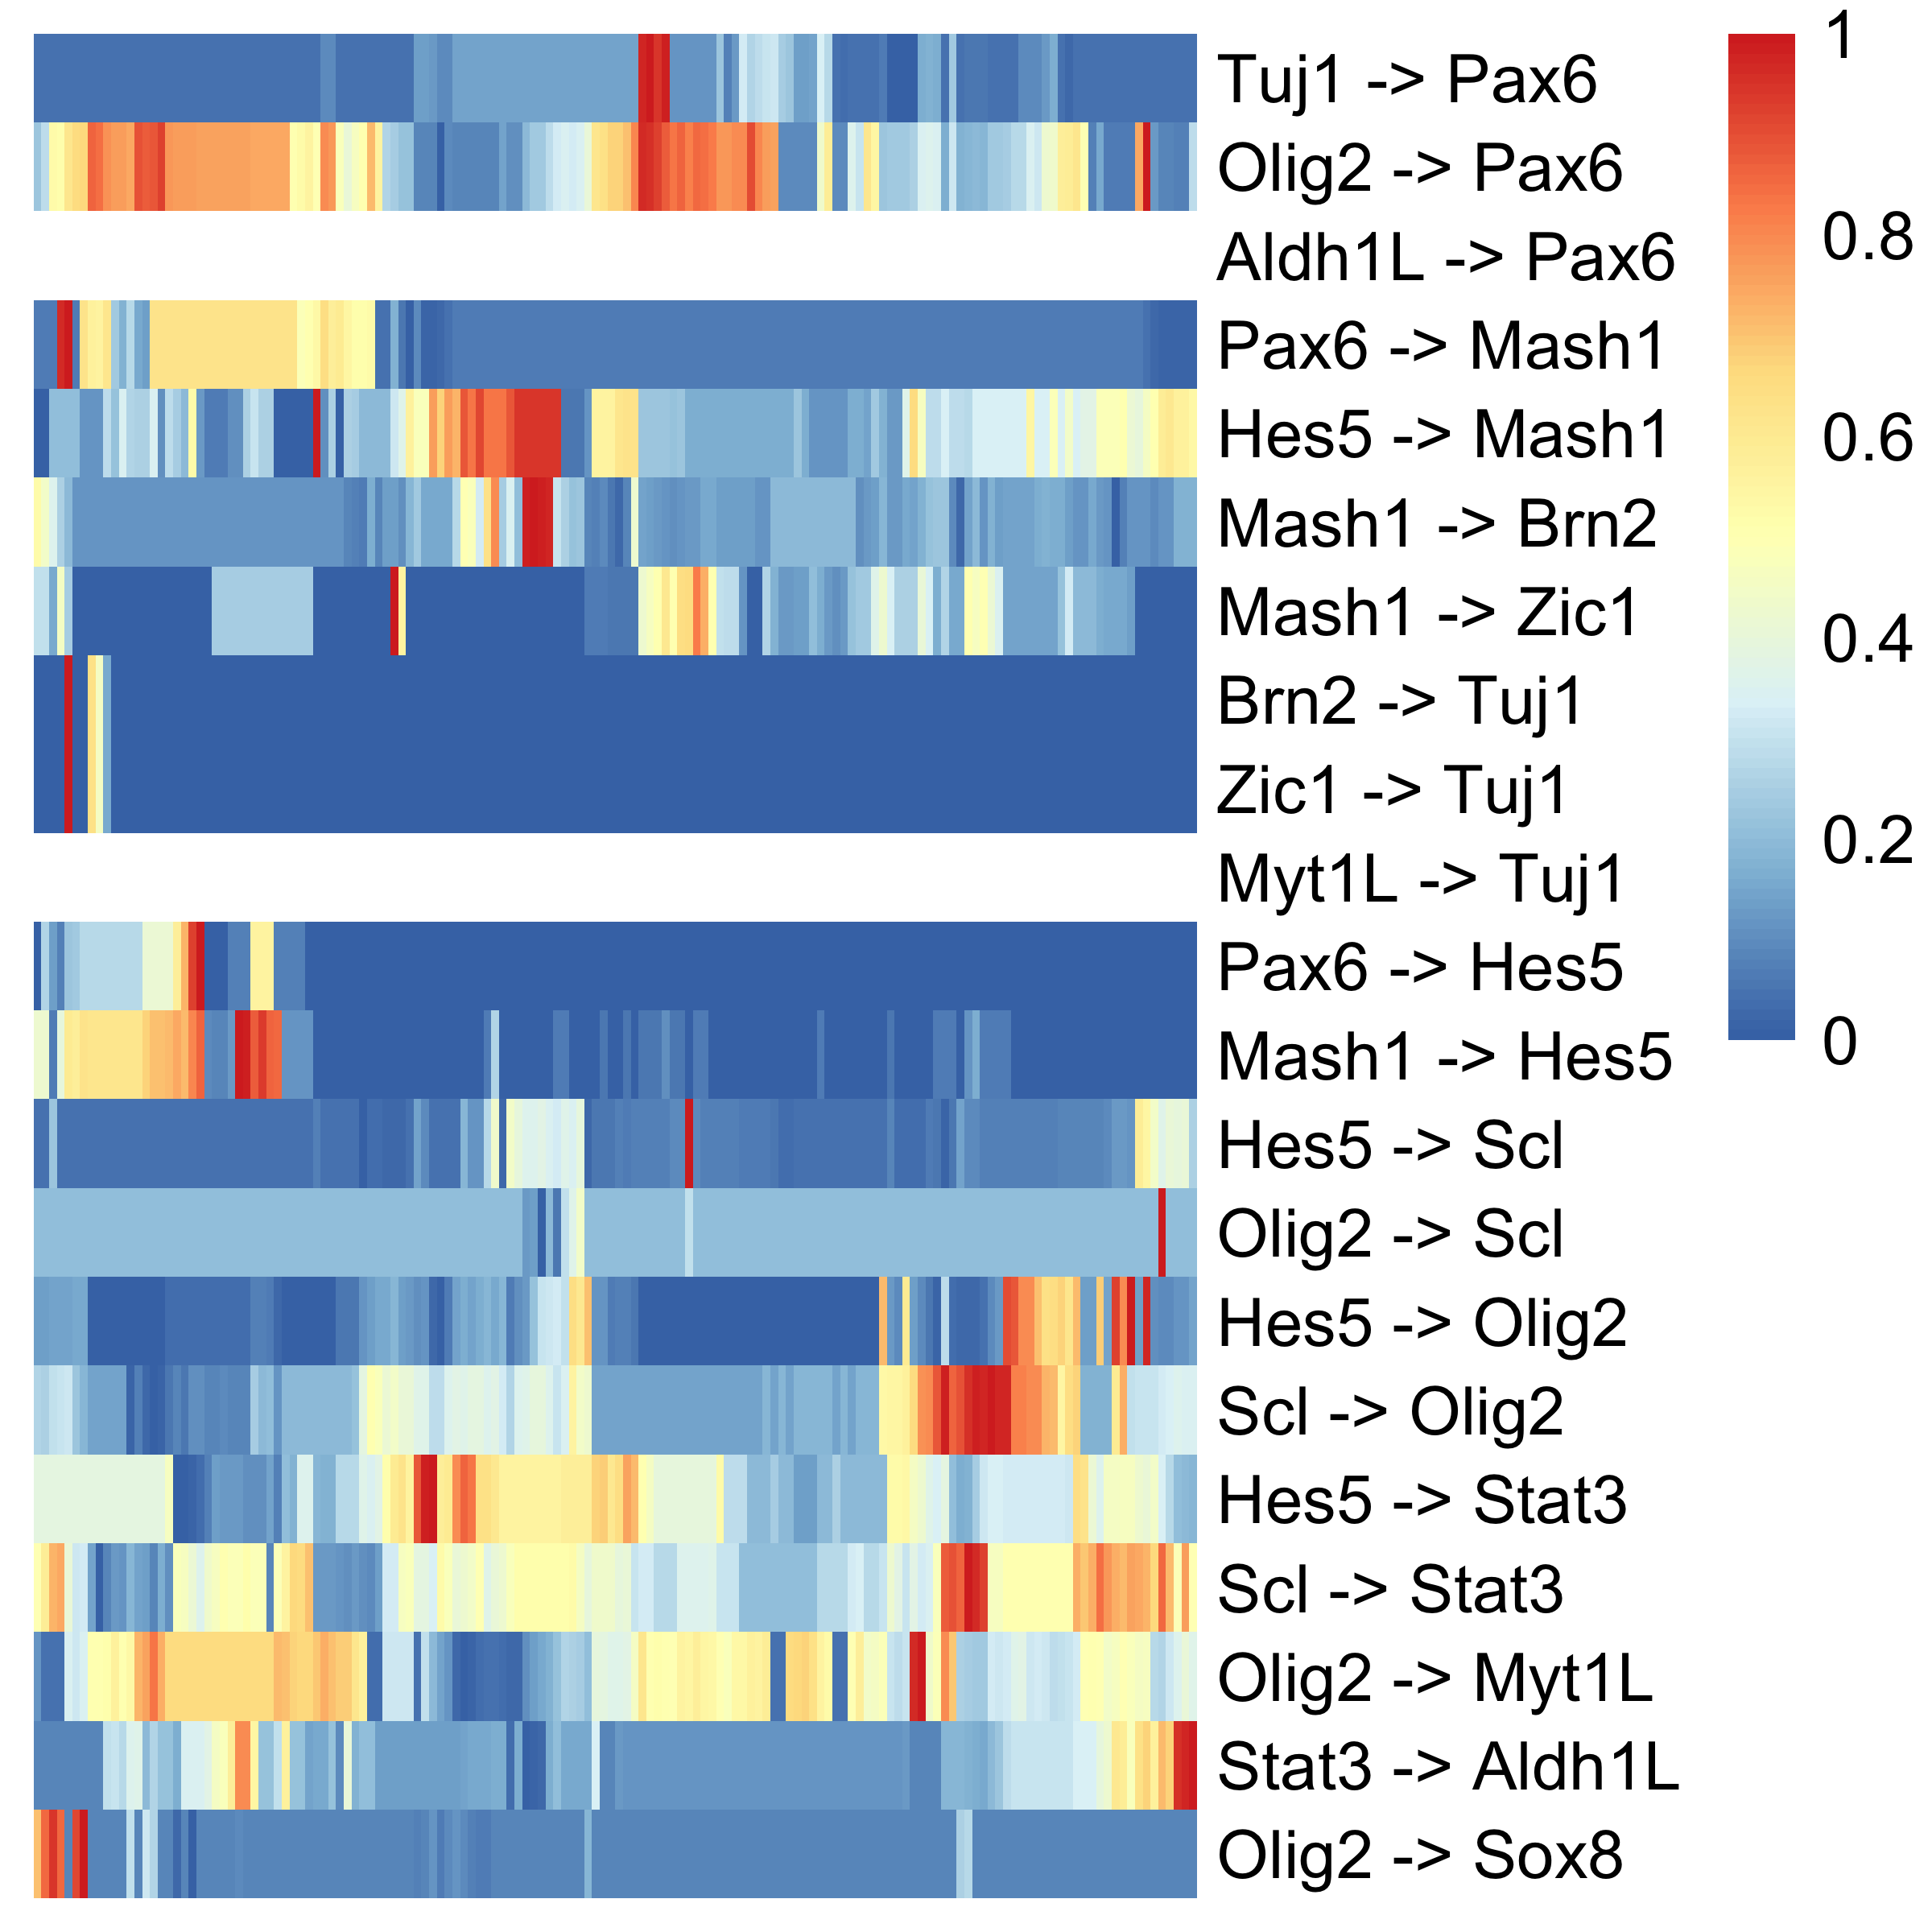
\includegraphics[width=\maxwidth]{figure/plot_temporal_rdi-4} 

}


\begin{kframe}\begin{alltt}
\hlstd{neuron_net} \hlkwb{<-} \hlkwd{graph_from_edgelist}\hlstd{(}\hlkwd{as.matrix}\hlstd{(neuron_network[,} \hlnum{1}\hlopt{:}\hlnum{2}\hlstd{]),} \hlkwc{directed} \hlstd{= T)}

\hlstd{layout_coord} \hlkwb{<-} \hlkwd{layout_as_tree}\hlstd{(neuron_net)}
\hlkwd{row.names}\hlstd{(layout_coord)} \hlkwb{<-} \hlkwd{V}\hlstd{(neuron_net)}\hlopt{$}\hlstd{name}
\hlstd{layout_coord[}\hlstr{"Tuj1"}\hlstd{, ]} \hlkwb{<-} \hlkwd{c}\hlstd{(}\hlopt{-}\hlnum{1.25}\hlstd{,}  \hlnum{0}\hlstd{)}

\hlstd{layout_coord[}\hlstr{"Scl"}\hlstd{, ]} \hlkwb{<-} \hlstd{layout_coord[}\hlstr{"Olig2"}\hlstd{, ]}
\hlstd{layout_coord[}\hlstr{"Olig2"}\hlstd{, ]} \hlkwb{<-} \hlkwd{c}\hlstd{(}\hlnum{1.25}\hlstd{,} \hlnum{1.00}\hlstd{)}
\hlstd{layout_coord[}\hlstr{"Stat3"}\hlstd{, ]} \hlkwb{<-} \hlkwd{c}\hlstd{(}\hlnum{0.4}\hlstd{,} \hlnum{0.5}\hlstd{)}
\hlstd{layout_coord[}\hlstr{"Aldh1L"}\hlstd{, ]} \hlkwb{<-} \hlkwd{c}\hlstd{(}\hlopt{-}\hlnum{0.75}\hlstd{,} \hlopt{-}\hlnum{1}\hlstd{)}
\hlstd{layout_coord[}\hlstr{"Myt1L"}\hlstd{, ]} \hlkwb{<-} \hlstd{layout_coord[}\hlstr{"Sox8"}\hlstd{, ]}
\hlstd{layout_coord[}\hlstr{"Sox8"}\hlstd{, ]} \hlkwb{<-} \hlkwd{c}\hlstd{(}\hlnum{1.95}\hlstd{,} \hlnum{0}\hlstd{)}

\hlstd{color} \hlkwb{=} \hlkwd{rep}\hlstd{(}\hlstr{'blue'}\hlstd{,} \hlnum{21}\hlstd{)}
\hlstd{color[}\hlkwd{c}\hlstd{(}\hlnum{5}\hlstd{,} \hlnum{12}\hlstd{,} \hlnum{14}\hlstd{,} \hlnum{16}\hlstd{)]} \hlkwb{<-} \hlstr{'red'}

\hlstd{res} \hlkwb{<-} \hlkwd{apply}\hlstd{(norm_valid_crdi_res,} \hlnum{2}\hlstd{,} \hlkwa{function}\hlstd{(}\hlkwc{x}\hlstd{)} \hlkwd{c}\hlstd{(}\hlkwd{mean}\hlstd{(x[}\hlnum{1}\hlopt{:}\hlnum{37}\hlstd{]),} \hlkwd{mean}\hlstd{(x[}\hlnum{38}\hlopt{:}\hlnum{64}\hlstd{]),} \hlkwd{mean}\hlstd{(x[}\hlnum{65}\hlopt{:}\hlnum{111}\hlstd{]),} \hlkwd{mean}\hlstd{(x[}\hlnum{112}\hlopt{:}\hlnum{150}\hlstd{])))}
\hlkwd{plot}\hlstd{(neuron_net,} \hlkwc{layout} \hlstd{= layout_coord,} \hlkwc{edge.width}\hlstd{=res[}\hlnum{1}\hlstd{, ]} \hlopt{*} \hlnum{5}\hlstd{,} \hlkwc{edge.color} \hlstd{= color)}
\end{alltt}
\end{kframe}

{\centering 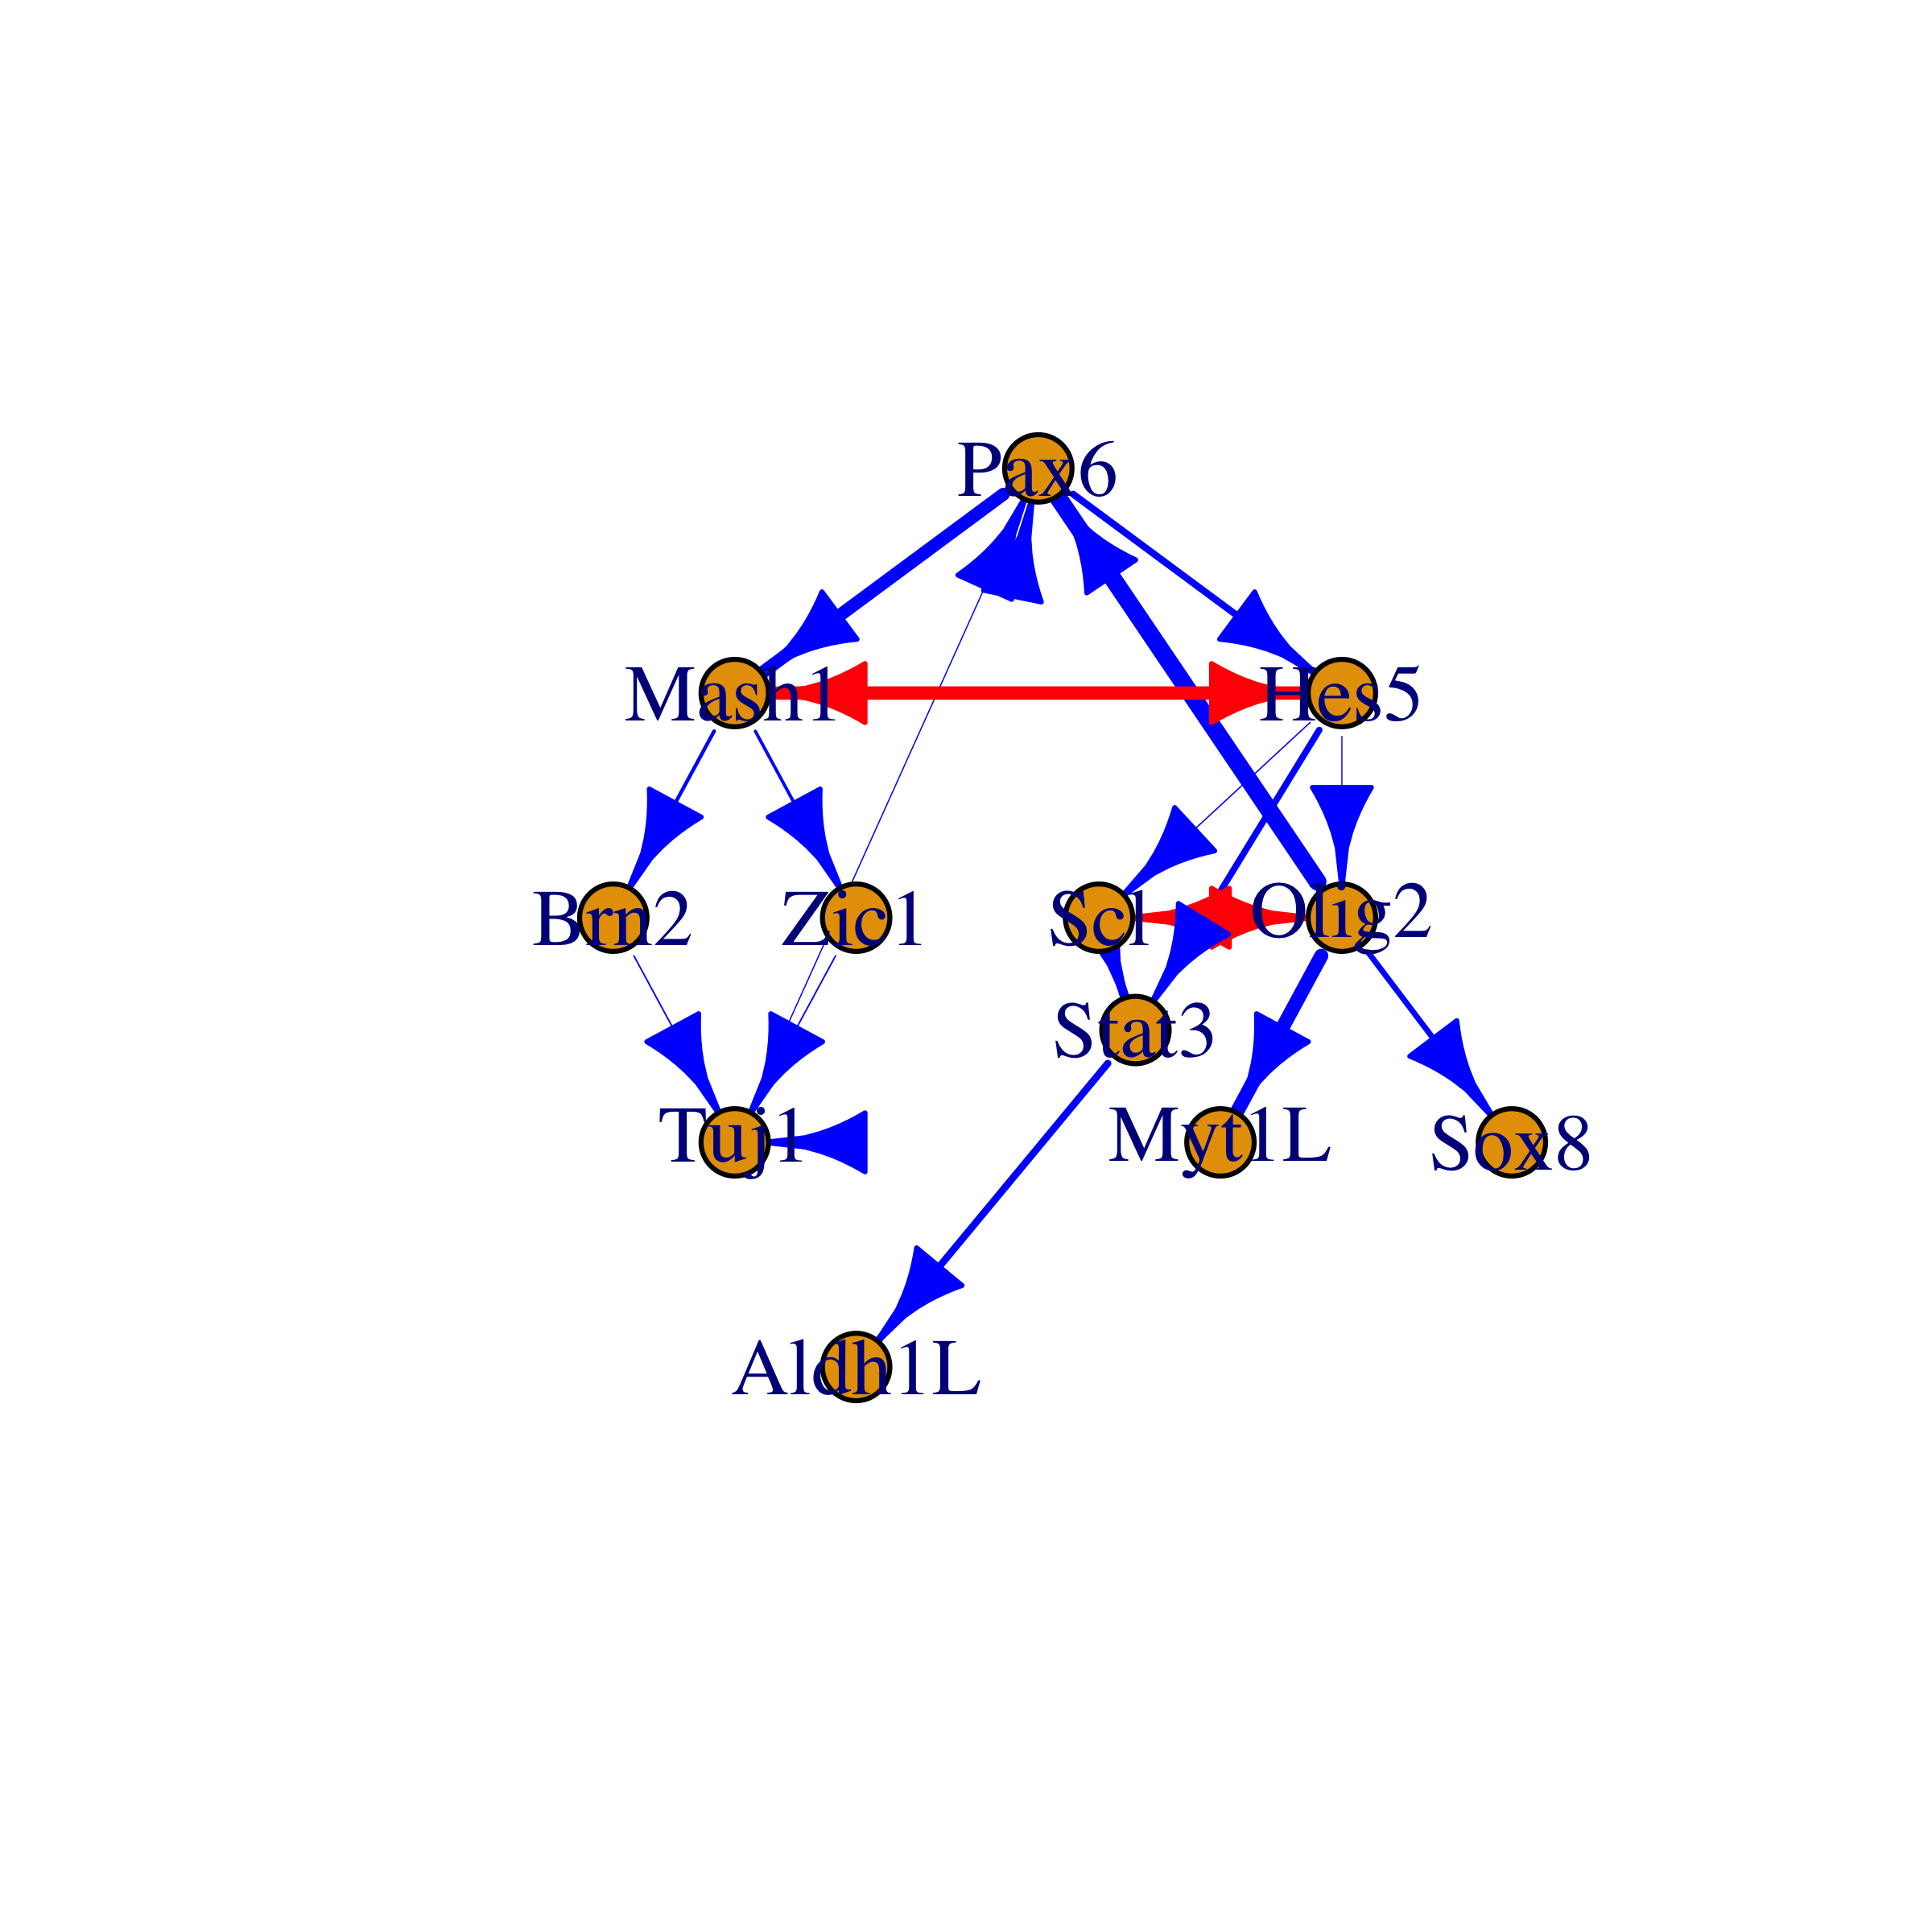
\includegraphics[width=\maxwidth]{figure/plot_temporal_rdi-5} 

}


\begin{kframe}\begin{alltt}
\hlkwd{plot}\hlstd{(neuron_net,} \hlkwc{layout} \hlstd{= layout_coord,} \hlkwc{edge.width}\hlstd{=res[}\hlnum{2}\hlstd{, ]} \hlopt{*} \hlnum{5}\hlstd{,} \hlkwc{edge.color} \hlstd{= color)}
\end{alltt}
\end{kframe}

{\centering 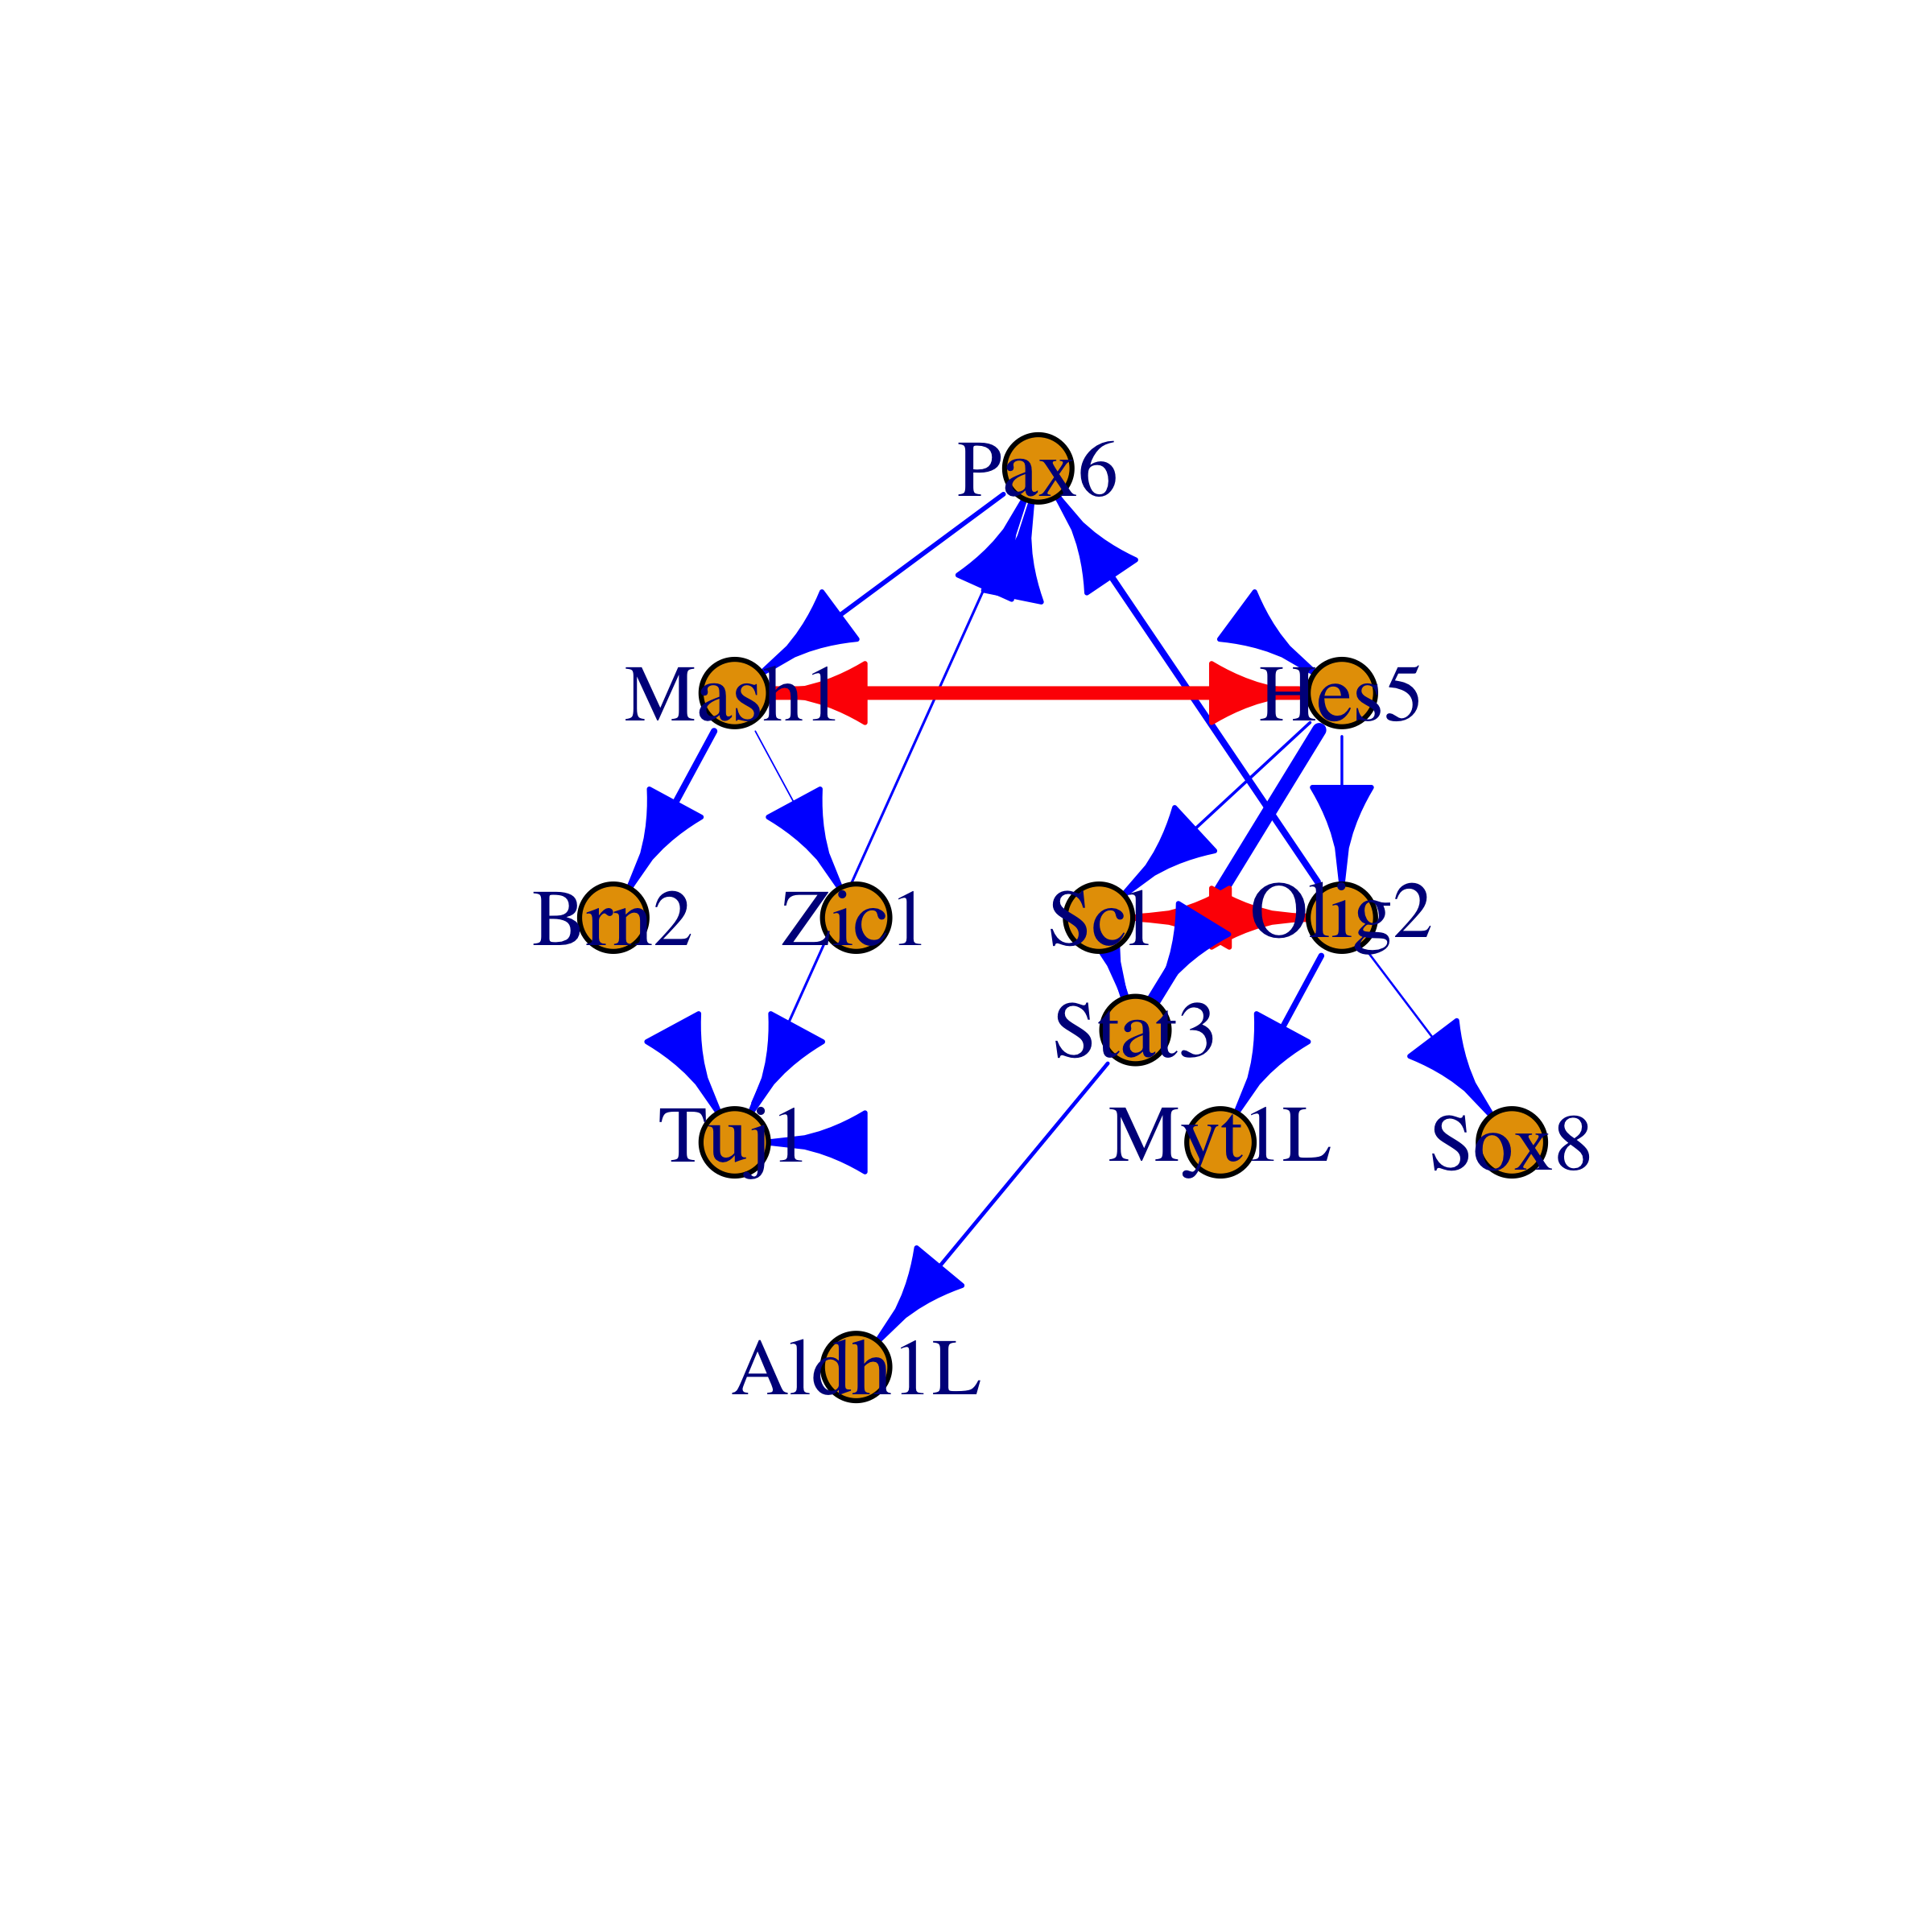
\includegraphics[width=\maxwidth]{figure/plot_temporal_rdi-6} 

}


\begin{kframe}\begin{alltt}
\hlkwd{plot}\hlstd{(neuron_net,} \hlkwc{layout} \hlstd{= layout_coord,} \hlkwc{edge.width}\hlstd{=res[}\hlnum{3}\hlstd{, ]} \hlopt{*} \hlnum{5}\hlstd{,} \hlkwc{edge.color} \hlstd{= color)}
\end{alltt}
\end{kframe}

{\centering 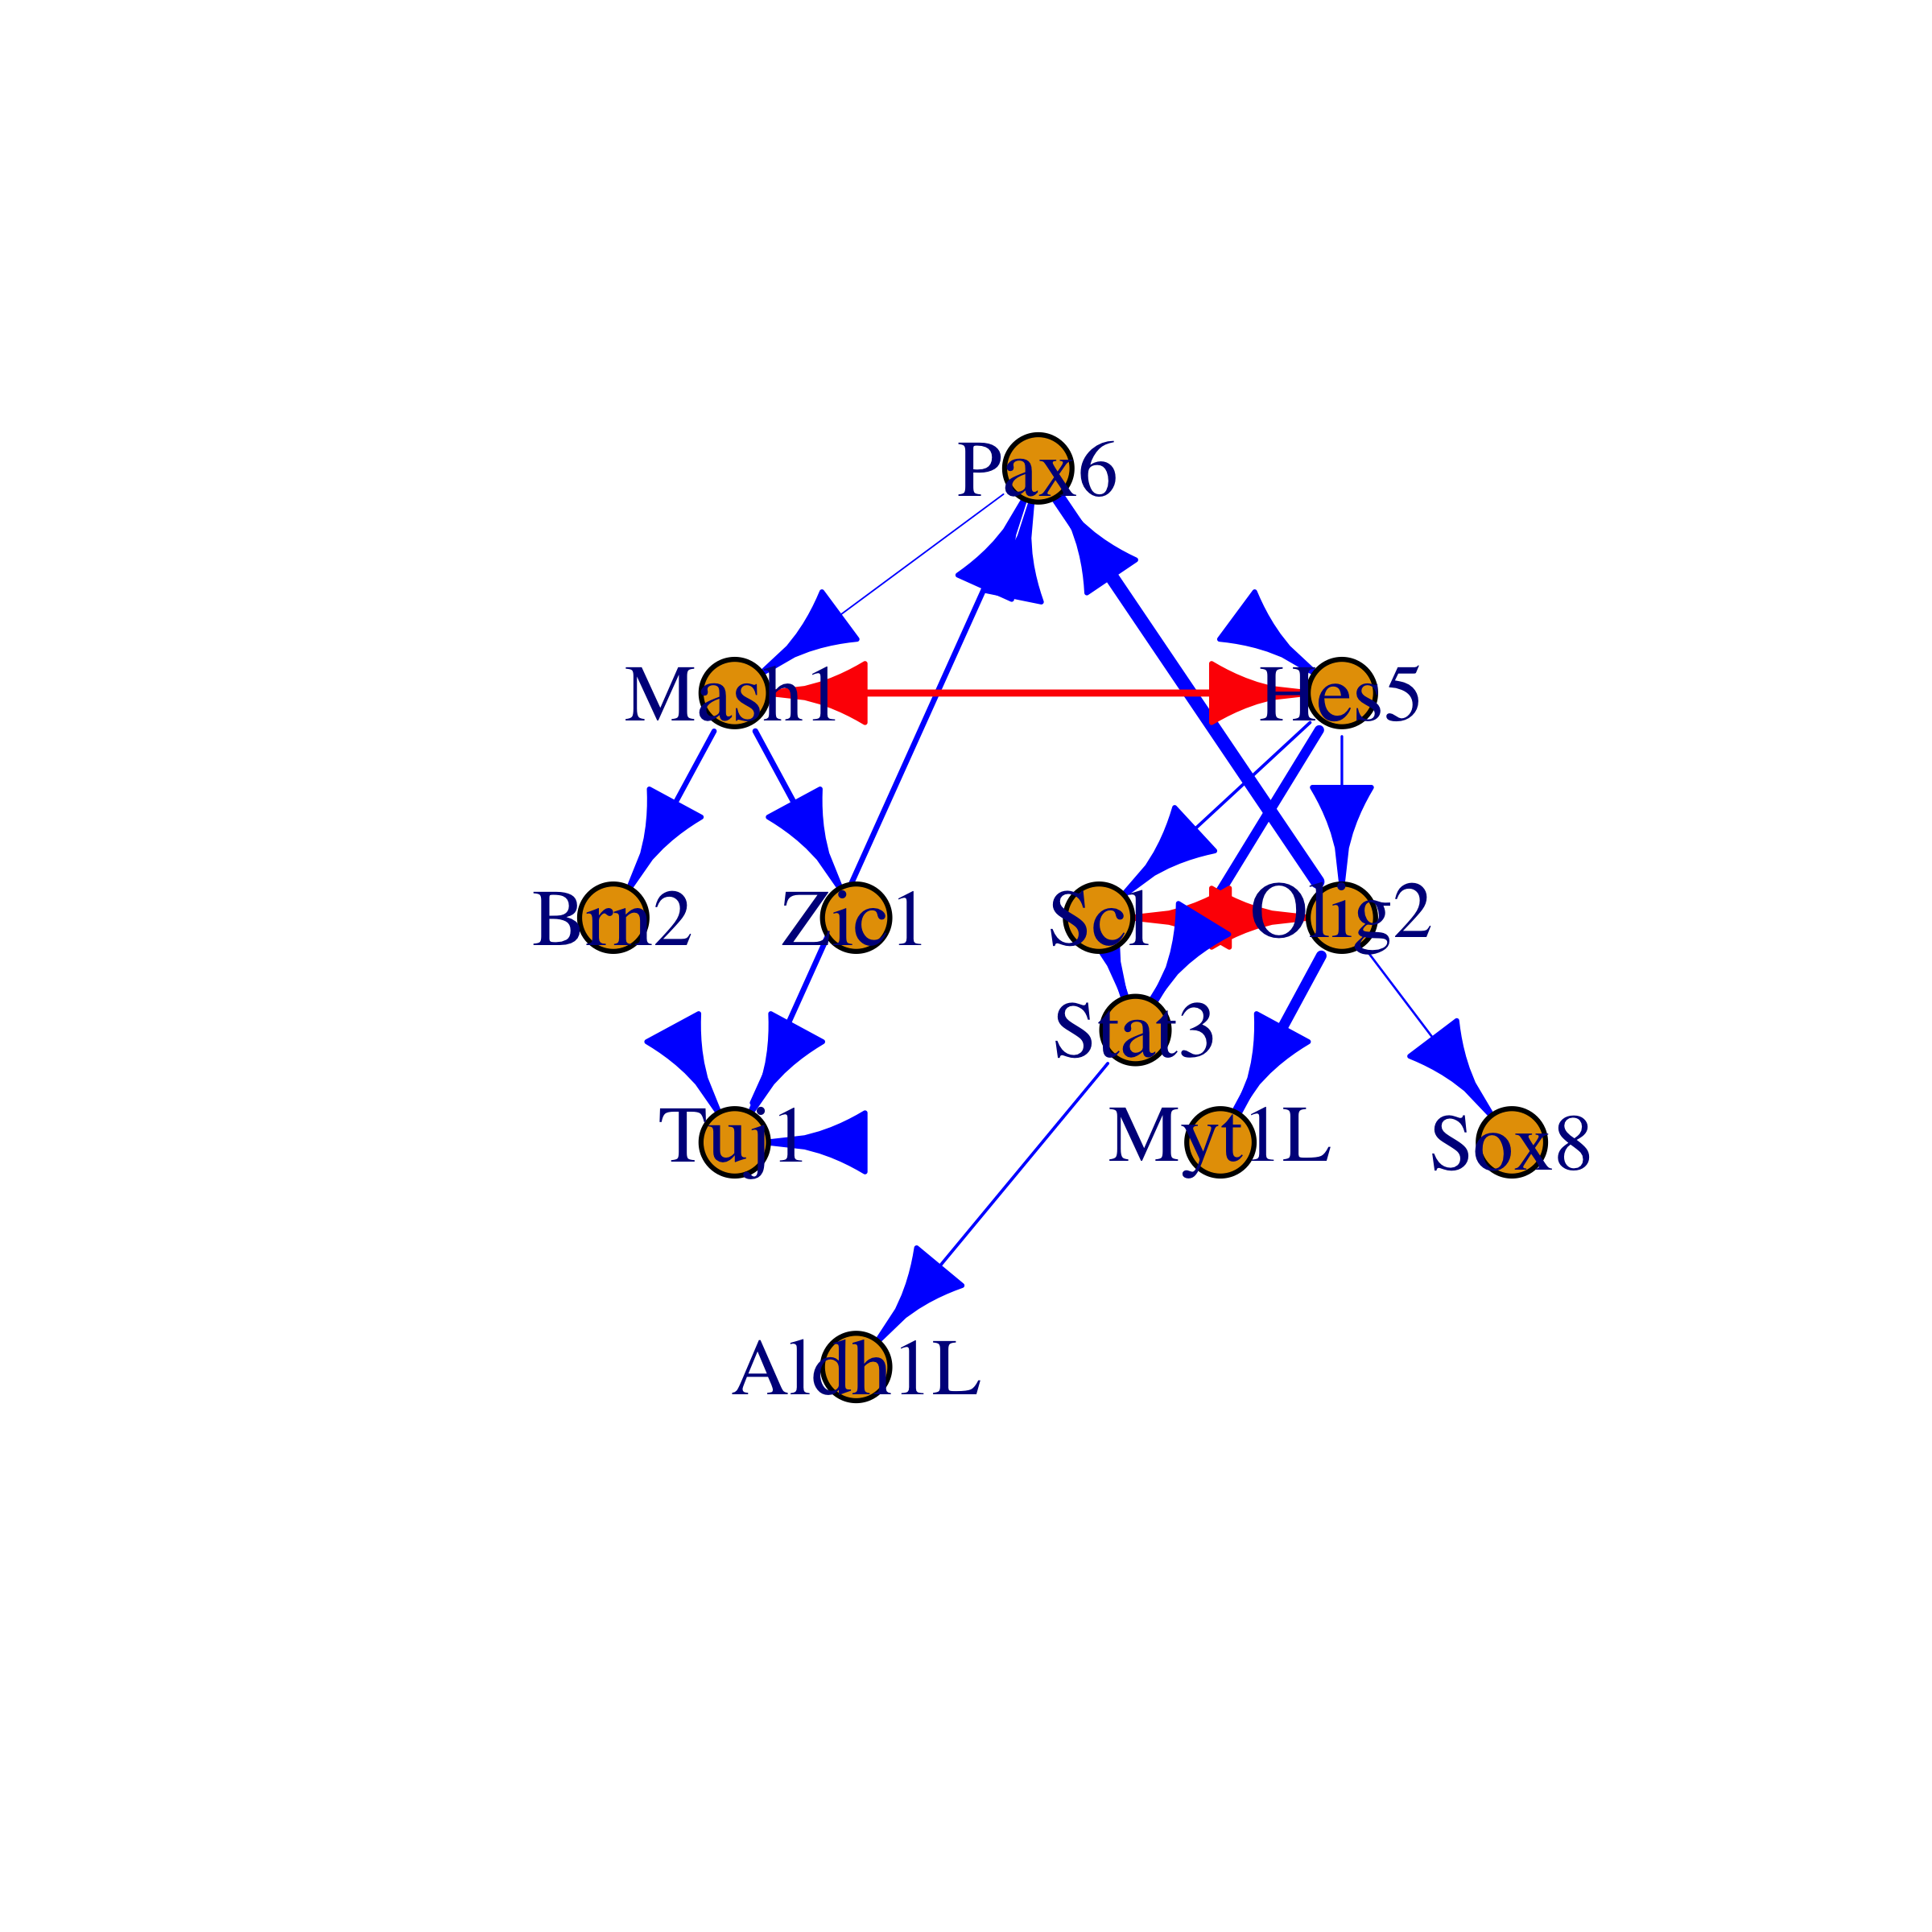
\includegraphics[width=\maxwidth]{figure/plot_temporal_rdi-7} 

}


\begin{kframe}\begin{alltt}
\hlkwd{plot}\hlstd{(neuron_net,} \hlkwc{layout} \hlstd{= layout_coord,} \hlkwc{edge.width}\hlstd{=res[}\hlnum{4}\hlstd{, ]} \hlopt{*} \hlnum{5}\hlstd{,} \hlkwc{edge.color} \hlstd{= color)}
\end{alltt}
\end{kframe}

{\centering 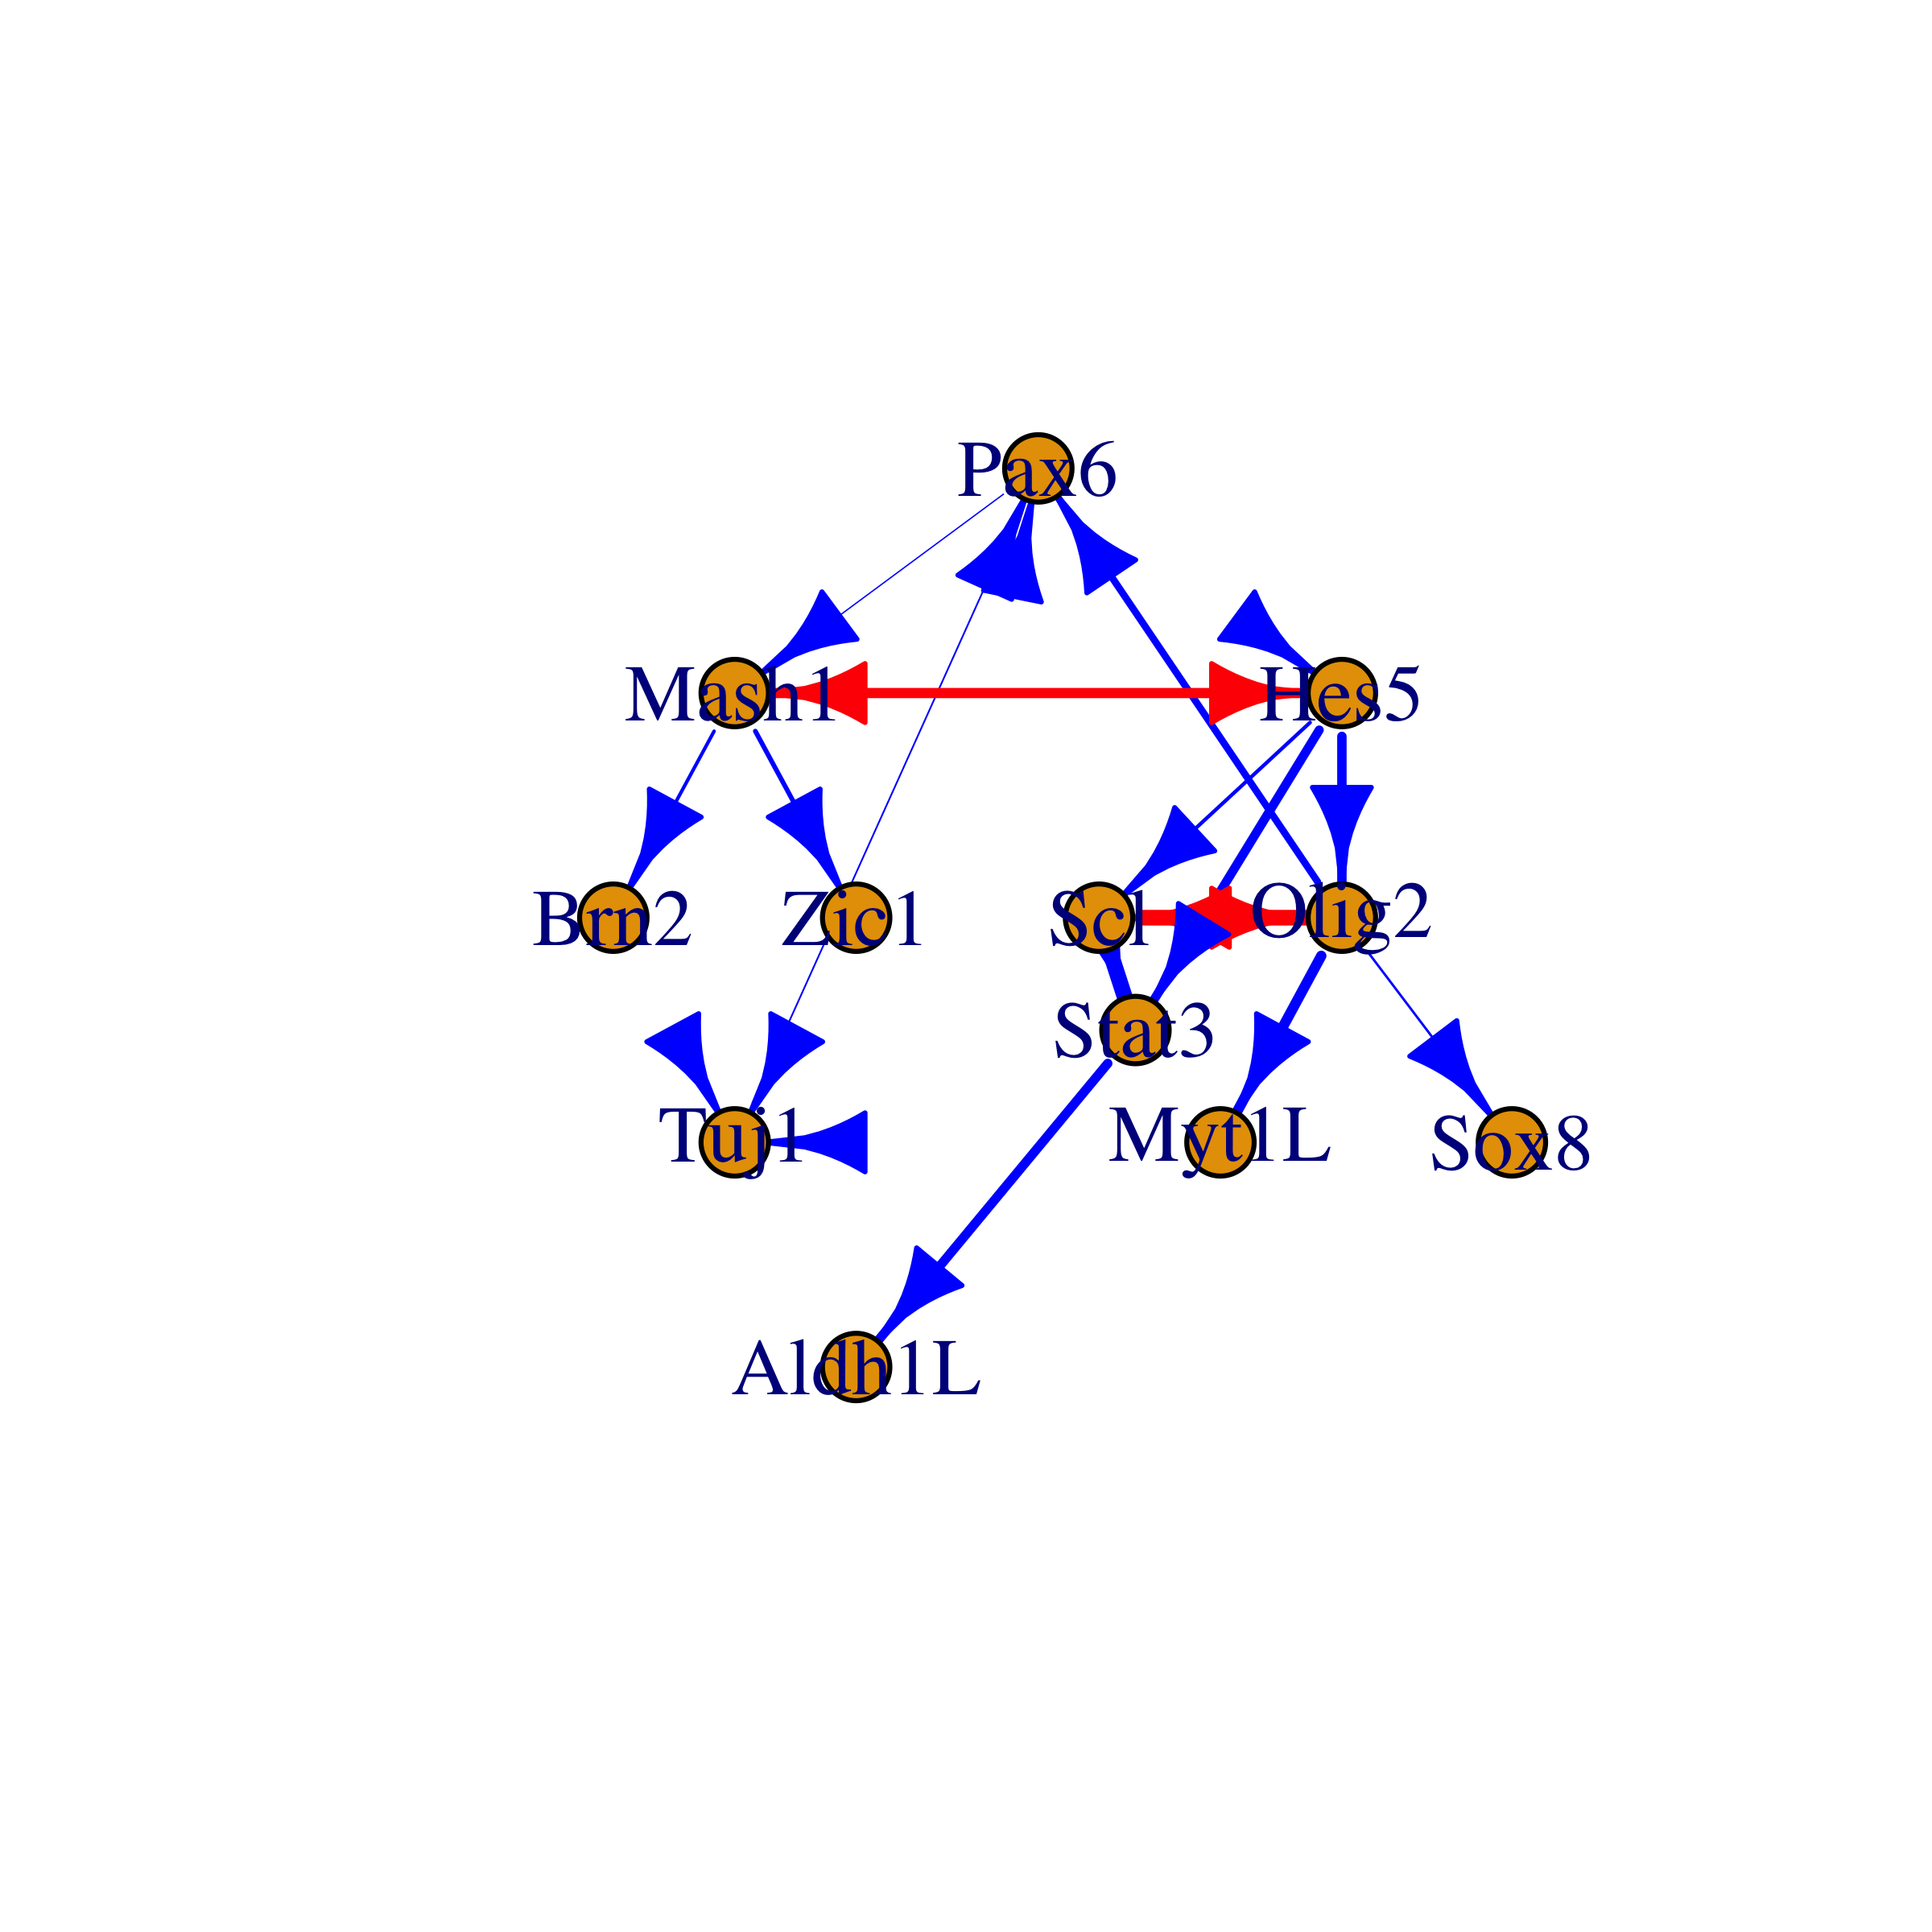
\includegraphics[width=\maxwidth]{figure/plot_temporal_rdi-8} 

}



\end{knitrout}

\subsection{Estimate time delay for gene pairs}

An important parameter required for causal network inference in Scribe is the proper time-delay between two genes. \Rpackage{Scribe} provides two empirical approaches to estimate this parameter: for the linear trajectory, \Rpackage{Scribe} identifies the inflection point for each gene and the difference between this two genes is used as the time delay; for a branch trajectory, \Rpackage{Scribe} identifies the branch time point for each gene and the difference between this two genes is used as the time delay. \textbf{estimate\_turning\_point} is the function to estimate the time delay between genes while the \textbf{plot\_time\_delay\_heatmap} can be used to visualize the time delay between any pairs of genes from the cds.

\begin{knitrout}
\definecolor{shadecolor}{rgb}{0.969, 0.969, 0.969}\color{fgcolor}\begin{kframe}
\begin{alltt}
\hlstd{na_sim_cds} \hlkwb{<-} \hlkwd{estimate_turning_point}\hlstd{(na_sim_cds)}
\hlkwd{plot_time_delay_heatmap}\hlstd{(na_sim_cds,} \hlkwc{use_gene_short_name} \hlstd{= F)}
\end{alltt}


{\ttfamily\noindent\itshape\color{messagecolor}{\#\# There is NA values in turining points calculated, the time delay is set to 0 by default}}\end{kframe}

{\centering 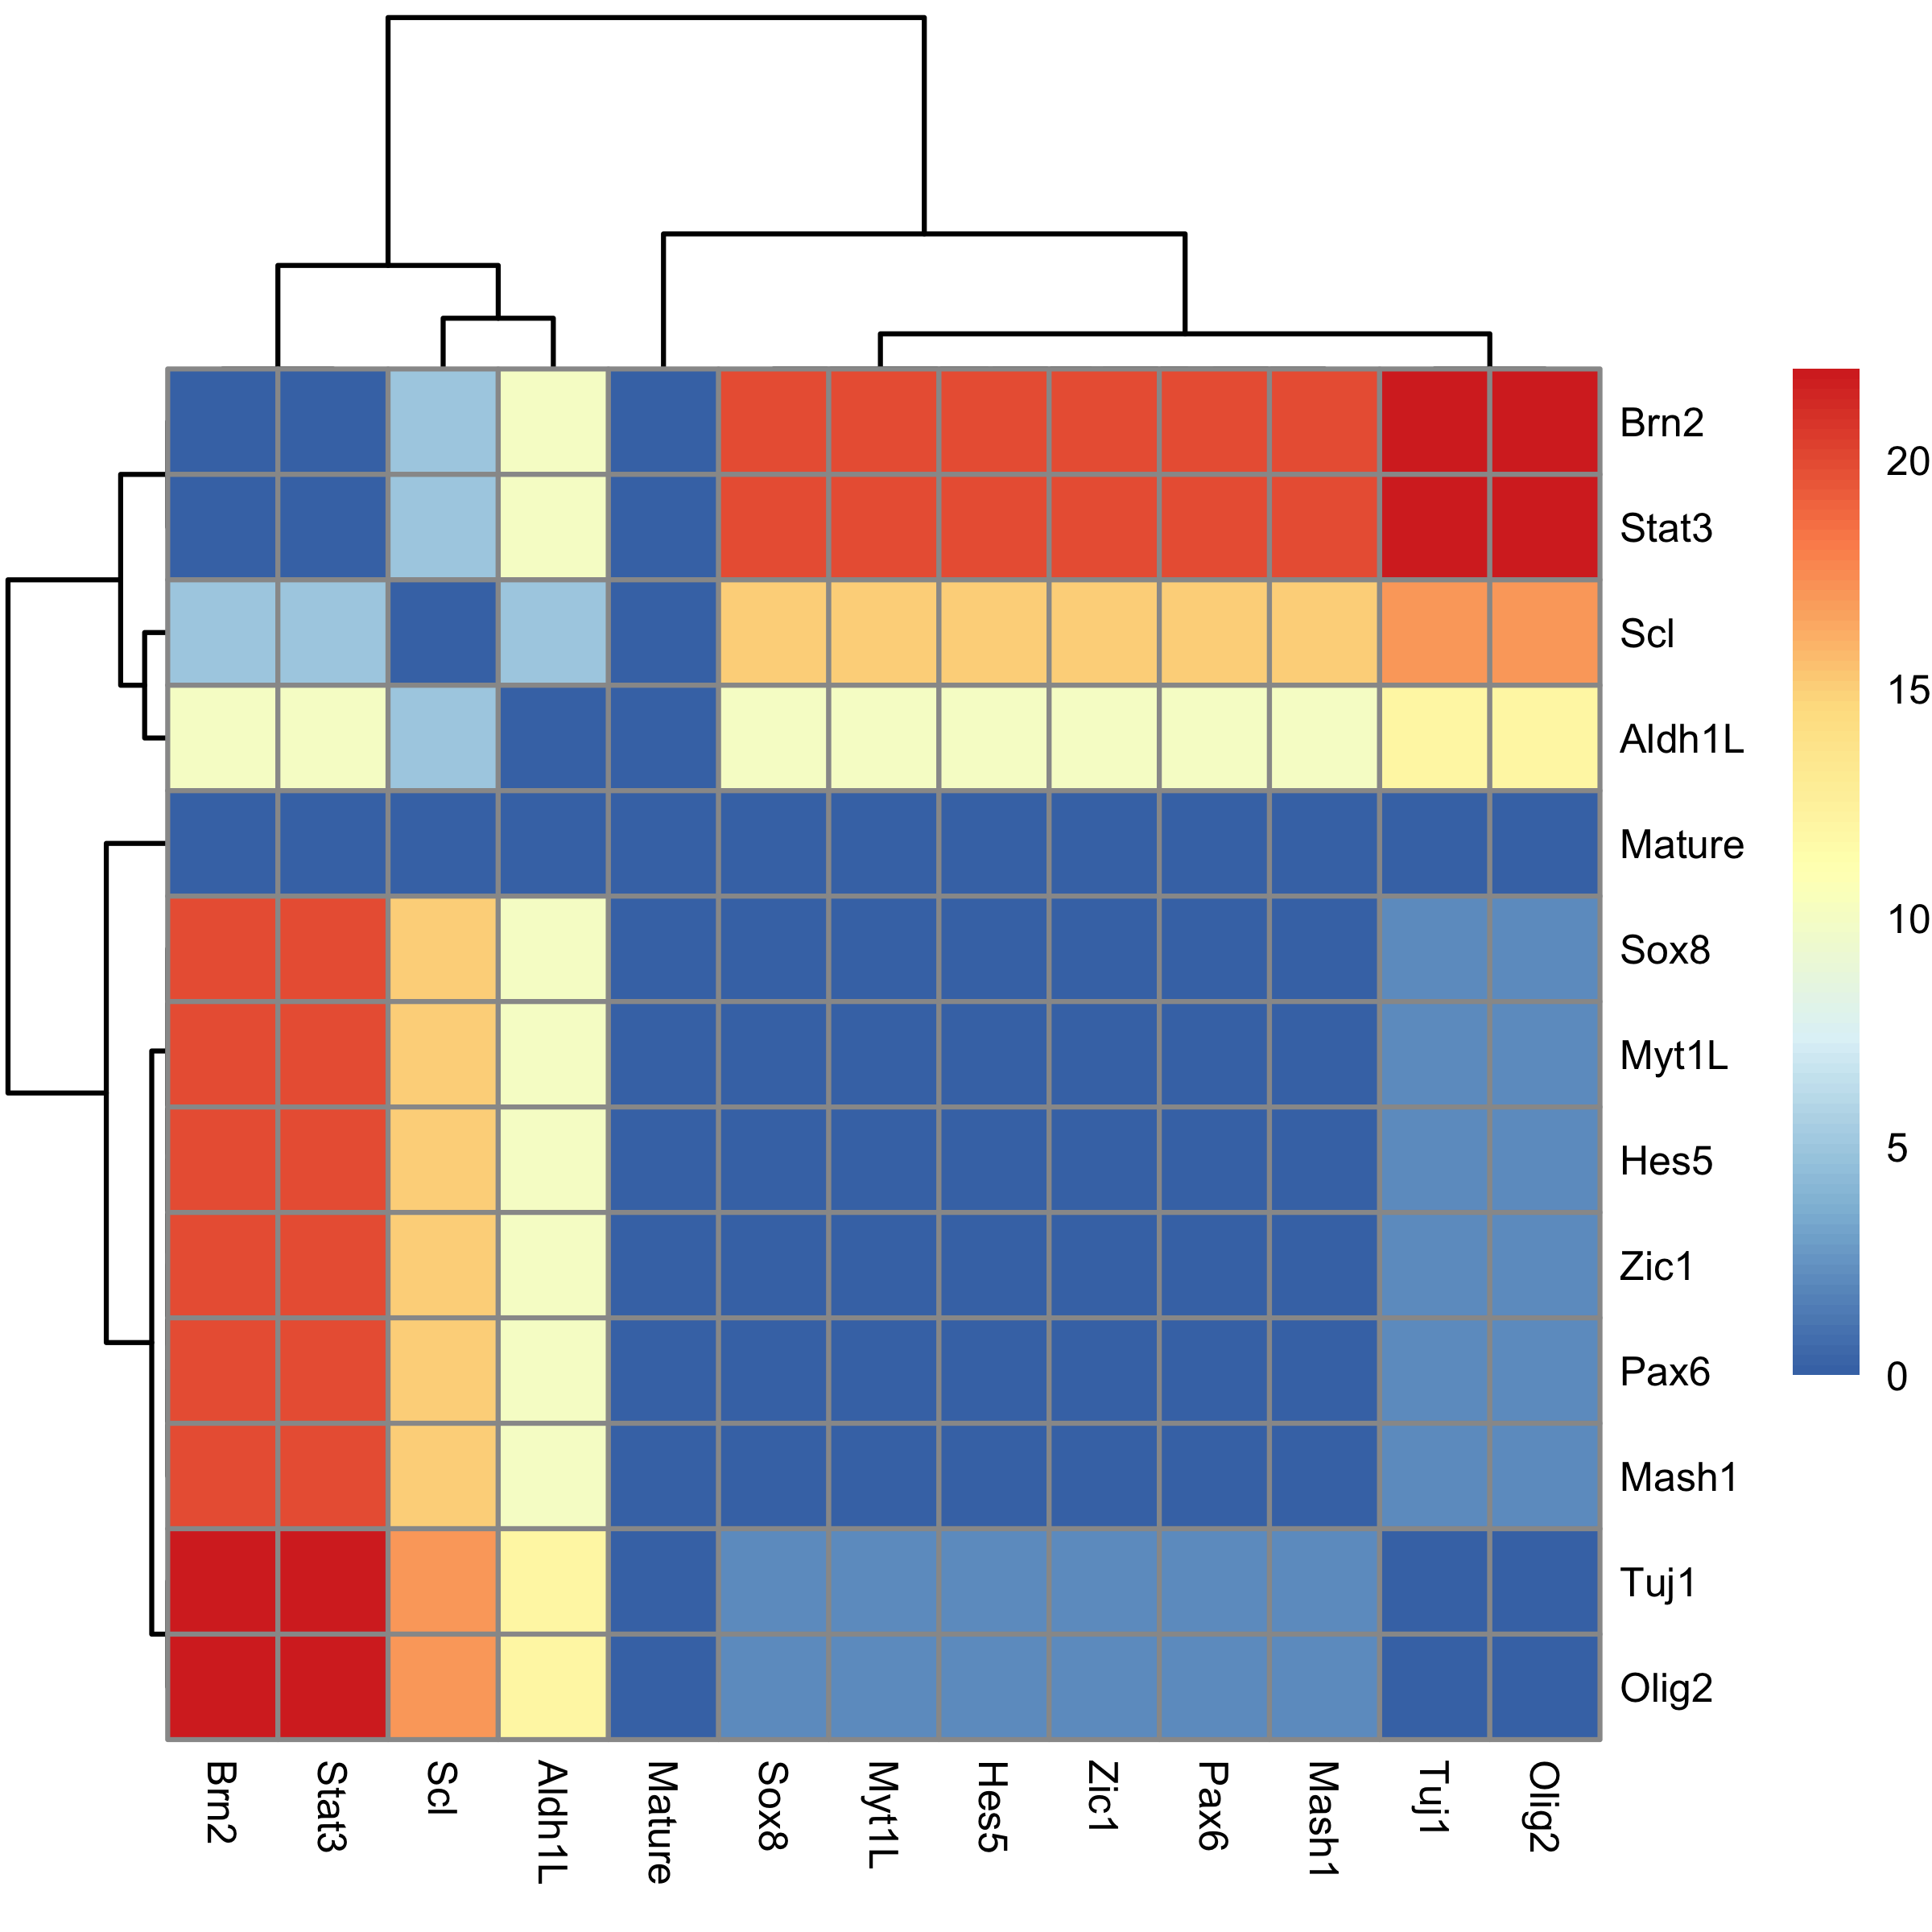
\includegraphics[width=\maxwidth]{figure/plot_time_delay_heatmap-1} 

}



\end{knitrout}

\subsection{Infer and visualize gene regulatory network}

We can infer the gene regulatory network through \textbf{calculate\_rdi\_multiple\_run\_cpp} function. This function will return a list with the following elements:
a. \textbf{RDI} (dimension is number of genes X length of delays times number of genes), vector of \textbf{delays}, \textbf{max\_rdi\_value} and \textbf{max\_rdi\_delays} (the matrices for the all possible pairs of gene regulation). After we run \textbf{calculate\_rdi\_multiple\_run\_cpp}, we can further calculate the conditional RDI values between all possible pair of genes by conditioning the top highest incoming node(s) based on the RDI results. \Rpackage{Scribe} can concatenate multiple directly related trajectory (for example different lineage commitment from the same developmental trajectory) for RDI calculation (that is why the term "multiple\_run" appears in the function). \Rpackage{Scribe} will also provide a procedure to sparsify the RDI/cRDI matrix to ensure  the distribution of indegree of the network follows the exponential distribution while the distribution of outdegree follows the power-law distribution (this part is still under development).

In \Rpackage{Scribe}, we provided a variety of approaches to visualize the RDI network we retrieved in the end. This can be done either by using the \Rpackage{heatmap}, \Rpackage{igraph} plotting function, the \Rpackage{hiearical} plot (based on \textbf{level.plot} in \Rpackage{netbiov} package), the arc diagram plot as well as the \Rpackage{Hive} plot.
\begin{knitrout}
\definecolor{shadecolor}{rgb}{0.969, 0.969, 0.969}\color{fgcolor}\begin{kframe}
\begin{alltt}
\hlstd{data} \hlkwb{<-} \hlkwd{t}\hlstd{(}\hlkwd{exprs}\hlstd{(neuron_sim_cds)[,} \hlnum{1}\hlopt{:}\hlnum{200}\hlstd{])} \hlcom{# prepare the data (row is sample, column is gene)}
\hlstd{noise} \hlkwb{=} \hlkwd{matrix}\hlstd{(}\hlkwd{rnorm}\hlstd{(}\hlkwc{mean} \hlstd{=} \hlnum{0}\hlstd{,} \hlkwc{sd} \hlstd{=} \hlnum{1e-10}\hlstd{,} \hlkwd{nrow}\hlstd{(data)} \hlopt{*} \hlkwd{ncol}\hlstd{(data)),} \hlkwc{nrow} \hlstd{=} \hlkwd{nrow}\hlstd{(data))}

\hlstd{run_vec} \hlkwb{<-} \hlkwd{rep}\hlstd{(}\hlnum{1}\hlstd{,} \hlkwd{nrow}\hlstd{(data))} \hlcom{# run information for each cell}

\hlcom{# create the network graph we want to estimate RDI (here we calculate all possible pair of gene regulation)}
\hlstd{tmp} \hlkwb{<-} \hlkwd{expand.grid}\hlstd{(}\hlnum{1}\hlopt{:}\hlkwd{ncol}\hlstd{(data),} \hlnum{1}\hlopt{:}\hlkwd{ncol}\hlstd{(data),} \hlkwc{stringsAsFactors} \hlstd{= F)}
\hlstd{super_graph} \hlkwb{<-} \hlstd{tmp[tmp[,} \hlnum{1}\hlstd{]} \hlopt{!=} \hlstd{tmp[,} \hlnum{2}\hlstd{], ]} \hlopt{-} \hlnum{1} \hlcom{#}
\hlstd{super_graph} \hlkwb{<-} \hlstd{super_graph[,} \hlkwd{c}\hlstd{(}\hlnum{2}\hlstd{,} \hlnum{1}\hlstd{)]}

\hlstd{rdi_list} \hlkwb{<-} \hlkwd{calculate_rdi_multiple_run_cpp}\hlstd{(data} \hlopt{+} \hlstd{noise,} \hlkwc{delay} \hlstd{=} \hlkwd{c}\hlstd{(}\hlnum{1}\hlstd{), run_vec} \hlopt{-} \hlnum{1}\hlstd{,} \hlkwd{as.matrix}\hlstd{(super_graph),} \hlkwc{method} \hlstd{=} \hlnum{1}\hlstd{,} \hlkwc{turning_points} \hlstd{=} \hlnum{0}\hlstd{)} \hlcom{#* 100 + noise}

\hlkwd{dimnames}\hlstd{(rdi_list}\hlopt{$}\hlstd{max_rdi_value)} \hlkwb{<-} \hlkwd{list}\hlstd{(gene_name_vec, gene_name_vec)}
\hlstd{con_rdi_res_test} \hlkwb{<-} \hlkwd{calculate_multiple_run_conditioned_rdi_wrap}\hlstd{(data} \hlopt{+} \hlstd{noise,} \hlkwd{as.matrix}\hlstd{(super_graph),} \hlkwd{as.matrix}\hlstd{(rdi_list}\hlopt{$}\hlstd{max_rdi_value),} \hlkwd{as.matrix}\hlstd{(rdi_list}\hlopt{$}\hlstd{max_rdi_delays), run_vec} \hlopt{-} \hlnum{1}\hlstd{,} \hlnum{1}\hlstd{)}
\hlkwd{dimnames}\hlstd{(con_rdi_res_test)} \hlkwb{<-} \hlkwd{list}\hlstd{(gene_name_vec, gene_name_vec)}

\hlcom{# visualize the network by heatmap}
\hlstd{pheatmap}\hlopt{::}\hlkwd{pheatmap}\hlstd{(rdi_list}\hlopt{$}\hlstd{max_rdi_value,} \hlkwc{cluster_rows} \hlstd{= F,} \hlkwc{cluster_cols} \hlstd{= F,} \hlkwc{annotation_names_col} \hlstd{= T,} \hlkwc{border_color} \hlstd{=} \hlnum{NA}\hlstd{)}
\end{alltt}
\end{kframe}

{\centering 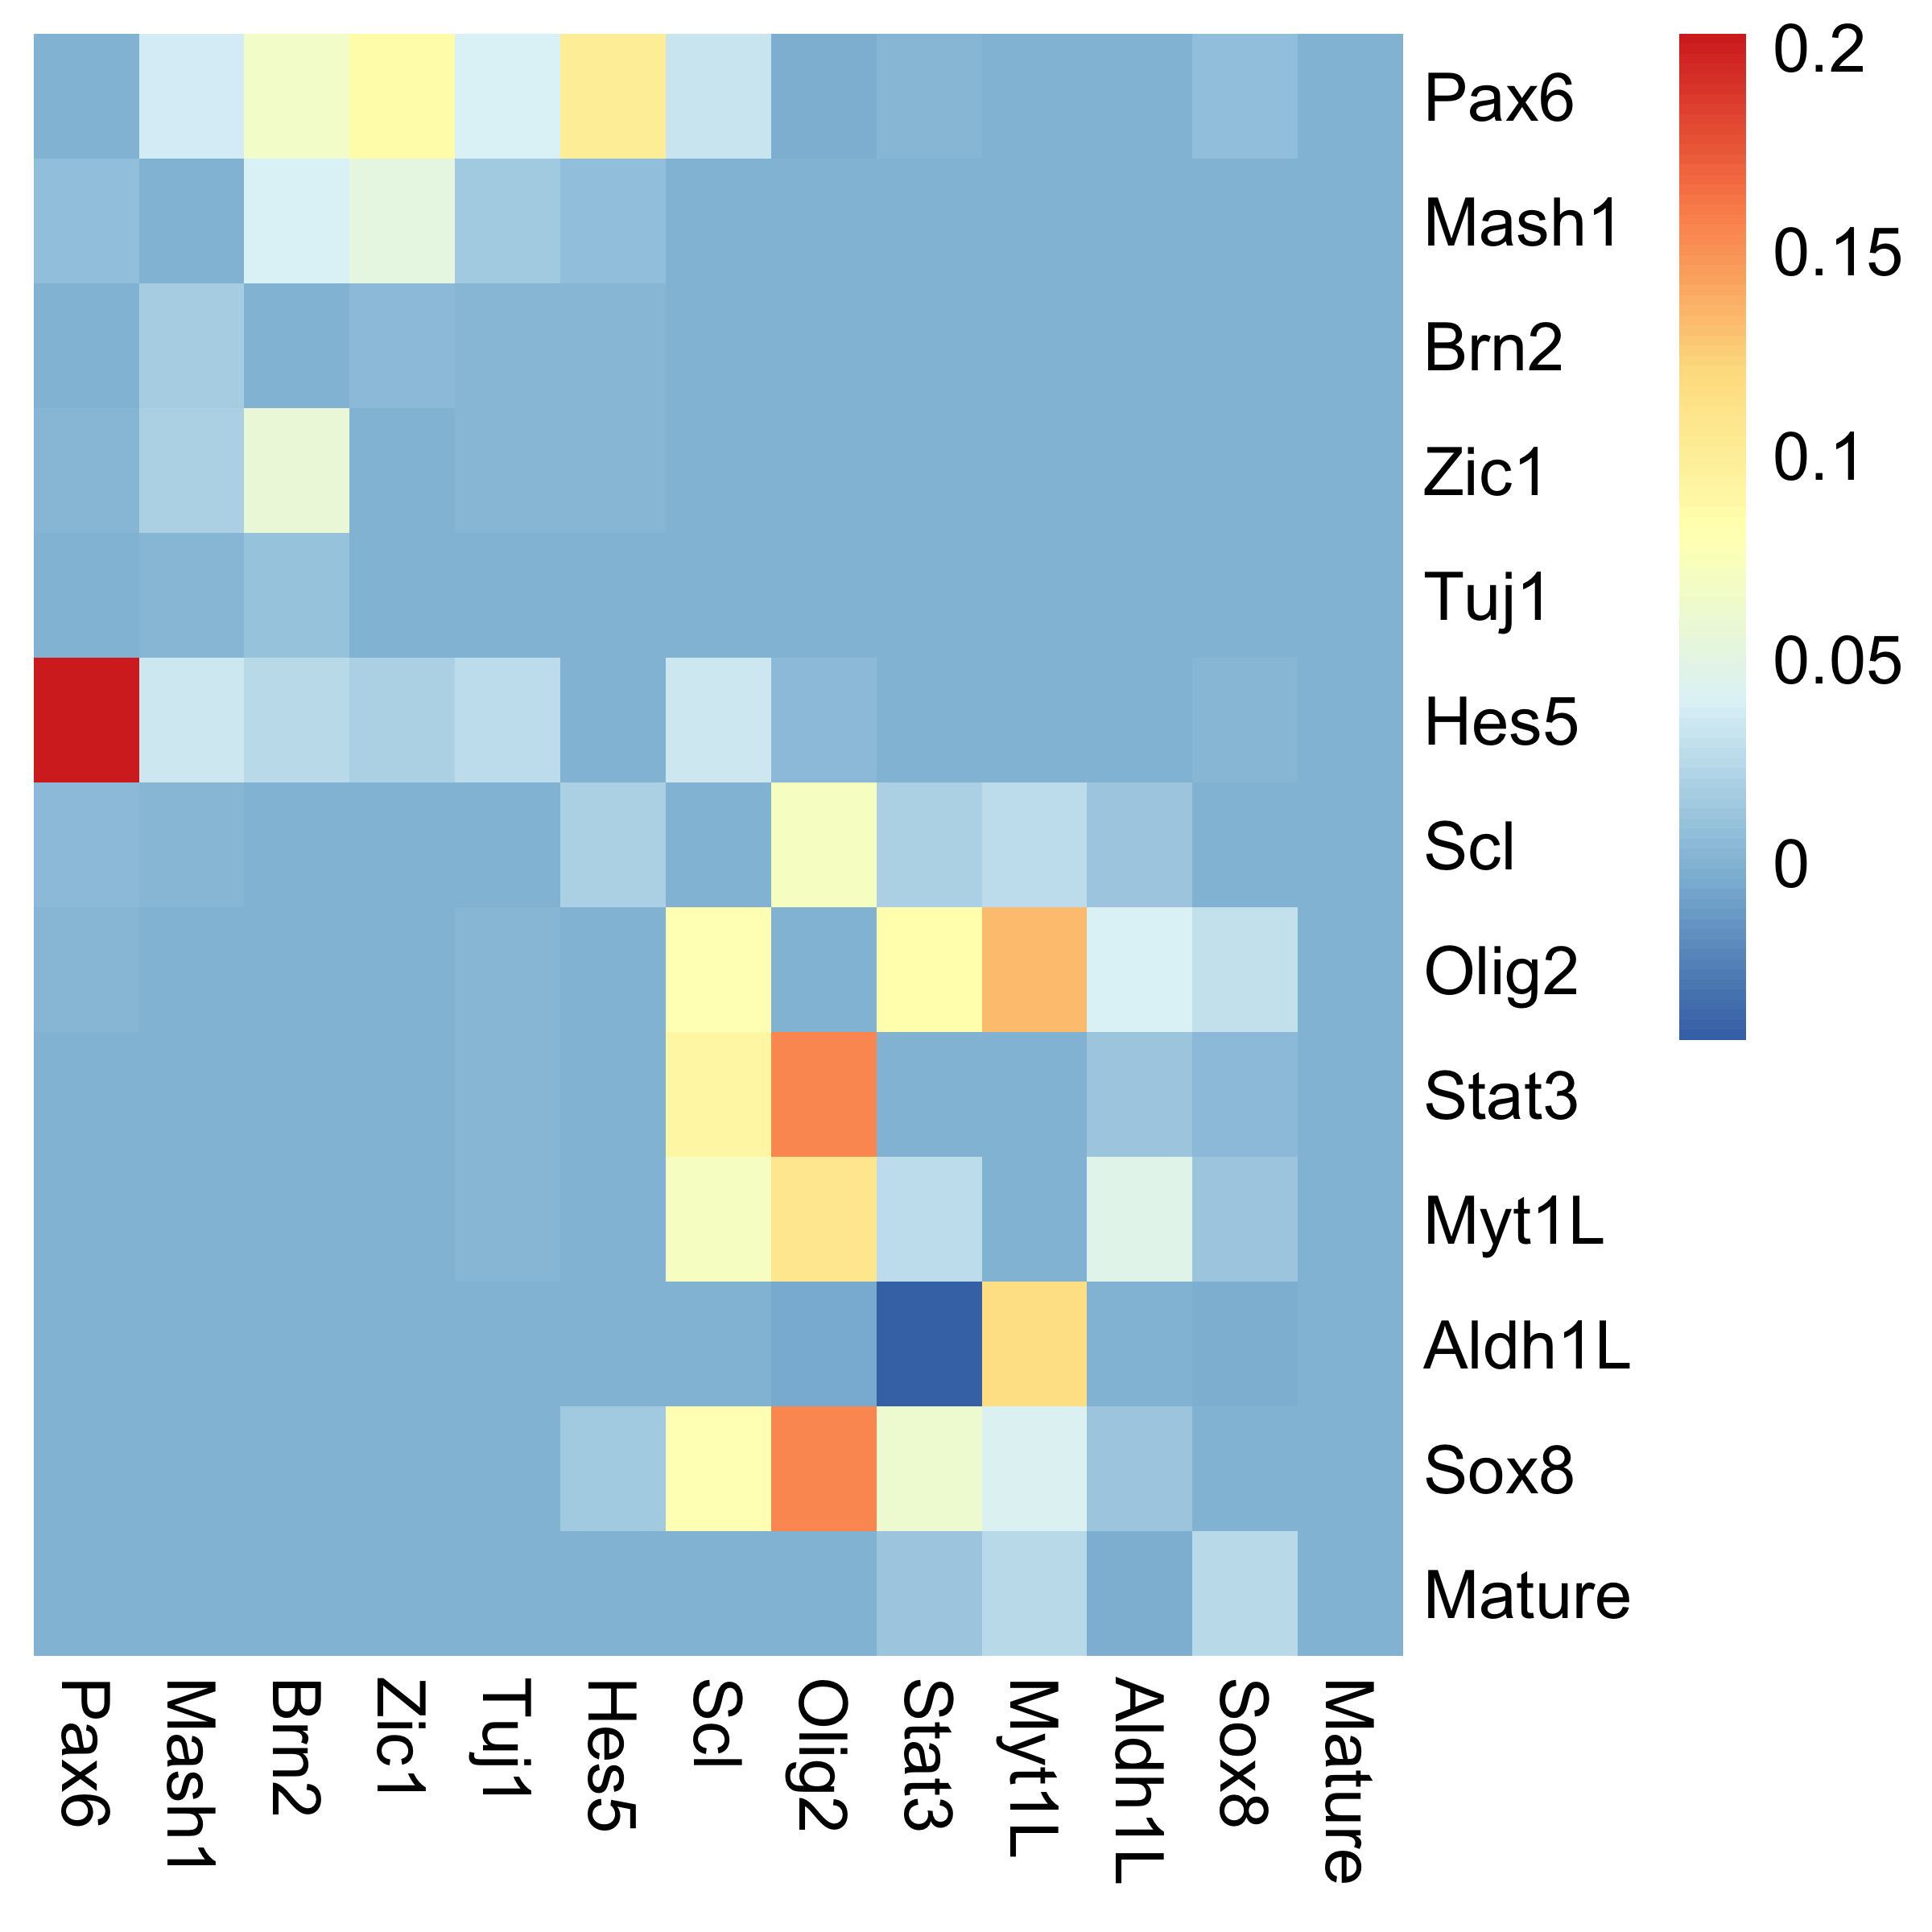
\includegraphics[width=\maxwidth]{figure/plot_network-1} 

}


\begin{kframe}\begin{alltt}
\hlstd{pheatmap}\hlopt{::}\hlkwd{pheatmap}\hlstd{(con_rdi_res_test,} \hlkwc{cluster_rows} \hlstd{= F,} \hlkwc{cluster_cols} \hlstd{= F,} \hlkwc{annotation_names_col} \hlstd{= T,} \hlkwc{border_color} \hlstd{=} \hlnum{NA}\hlstd{)}
\end{alltt}
\end{kframe}

{\centering 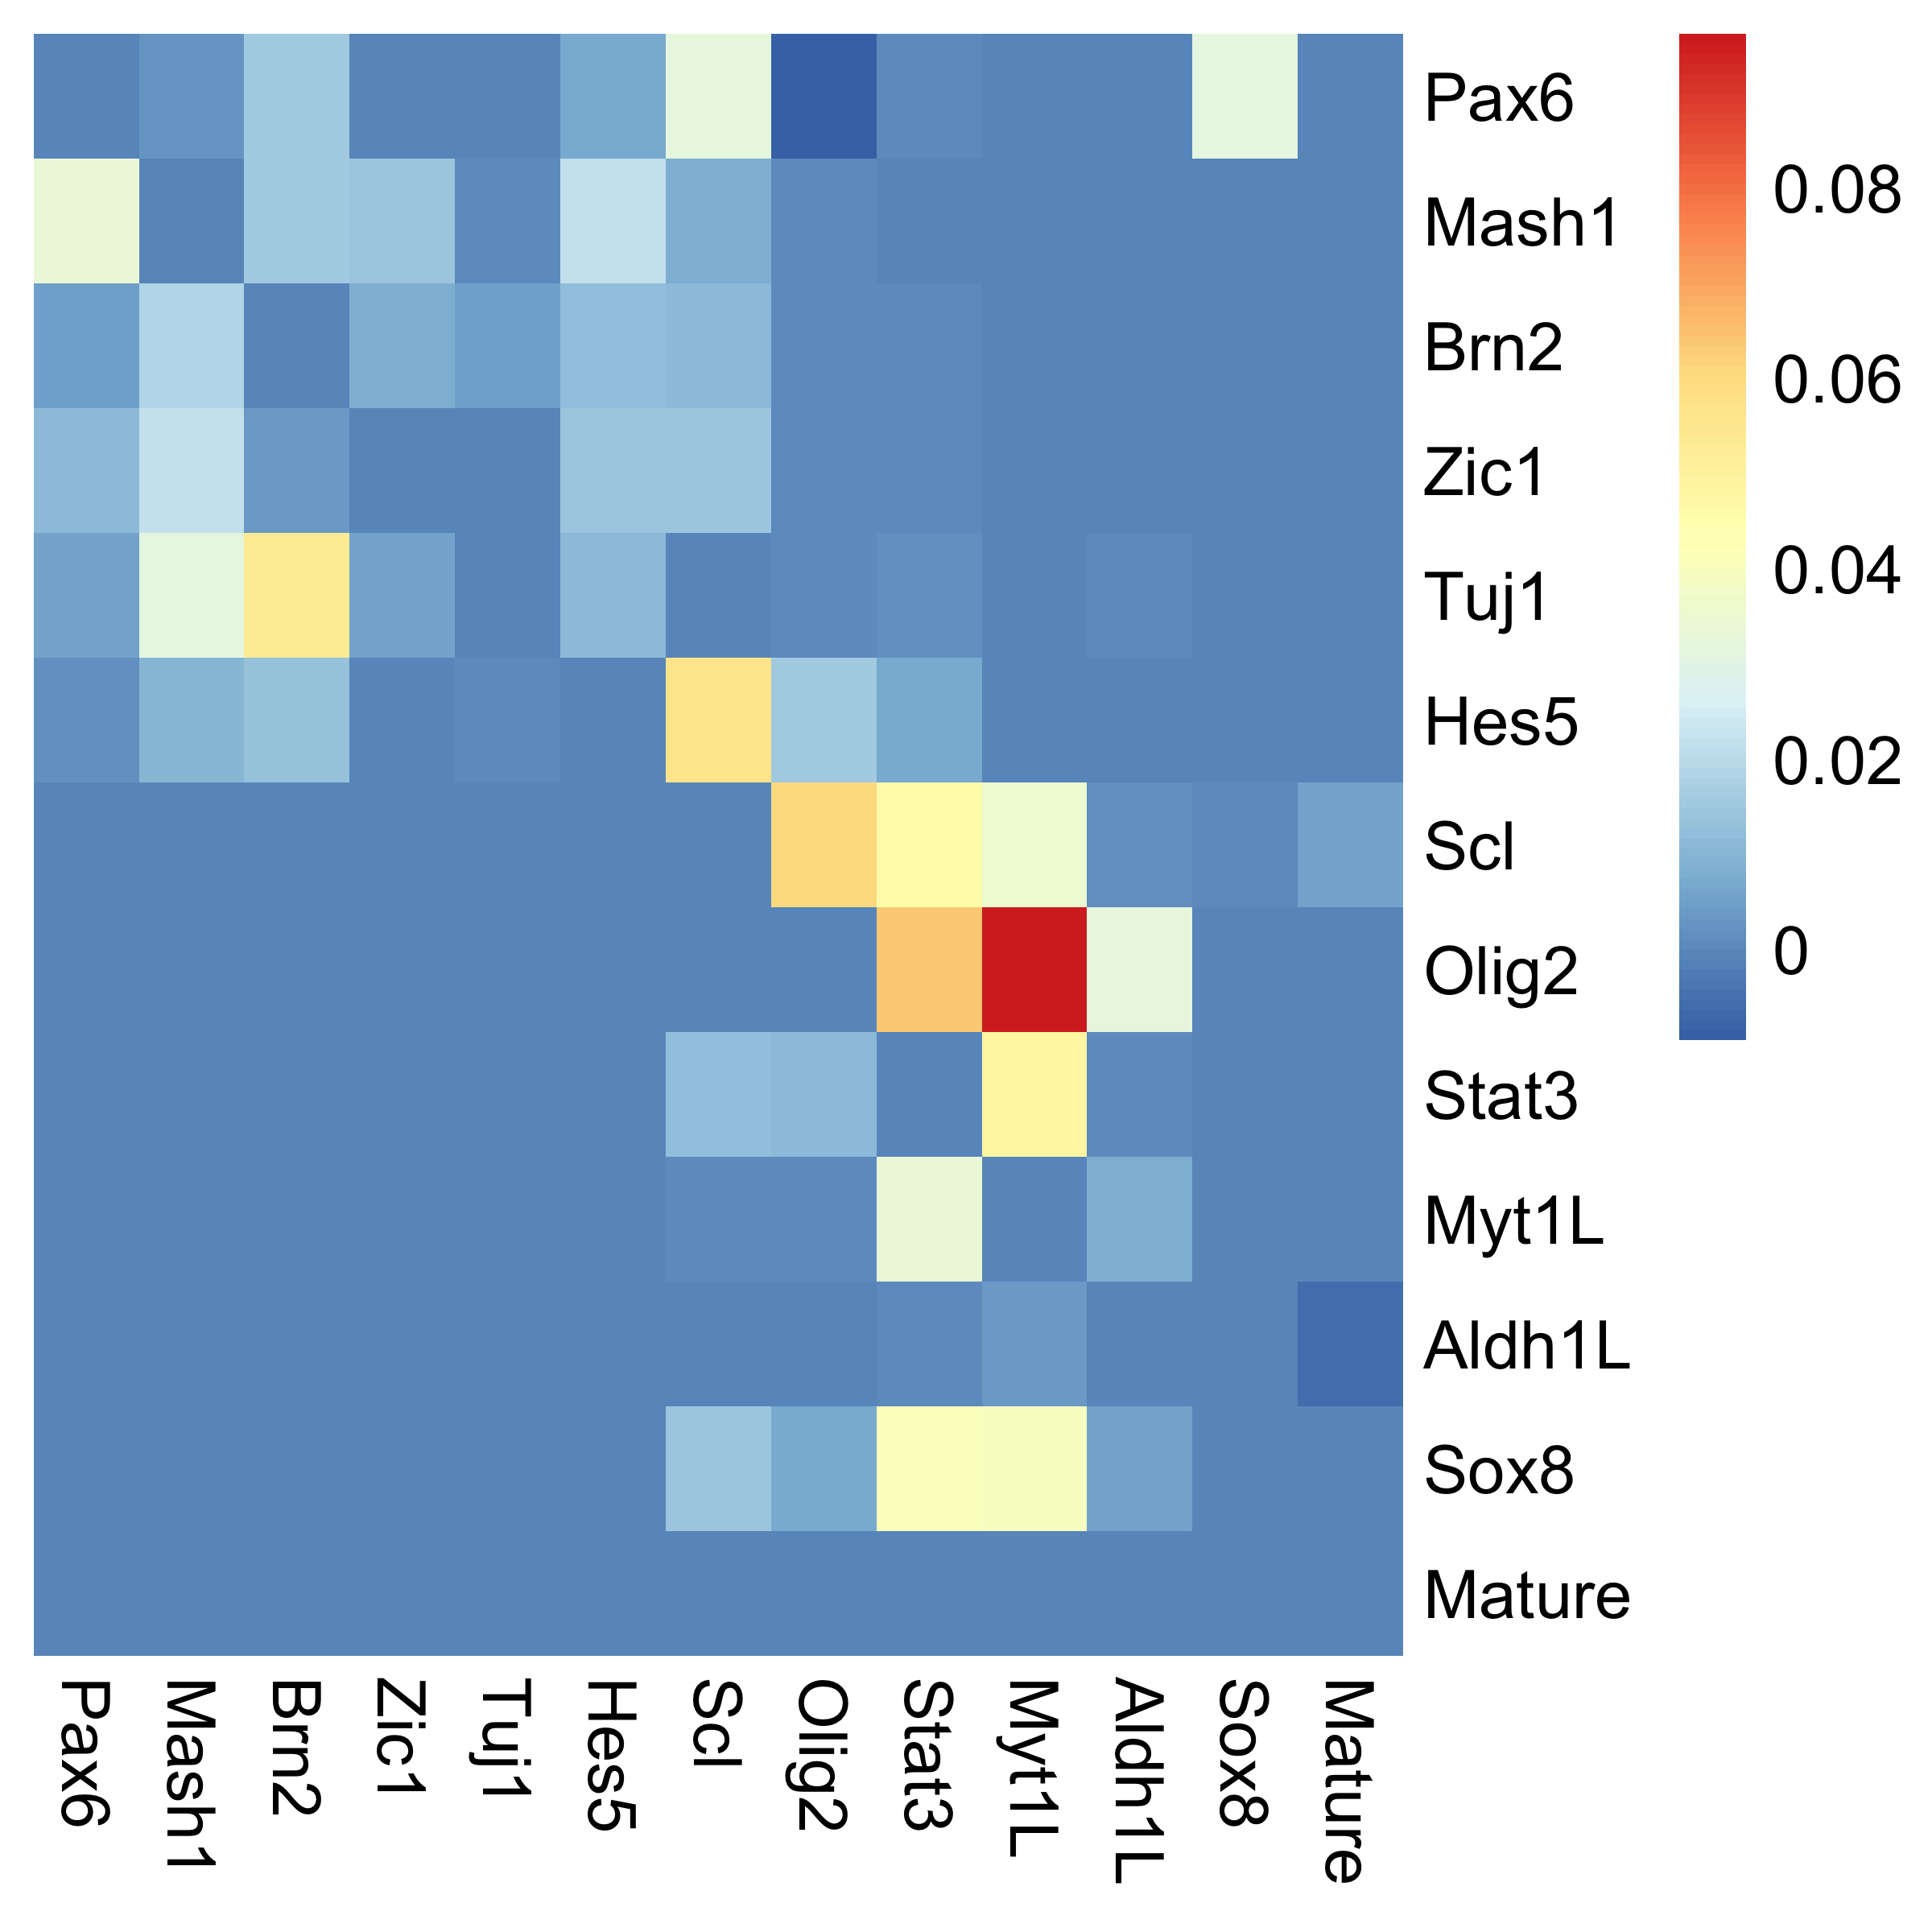
\includegraphics[width=\maxwidth]{figure/plot_network-2} 

}


\begin{kframe}\begin{alltt}
\hlcom{# in the following, I will show how to visualize a large scale network}
\hlcom{# load the network:}
\hlkwd{load}\hlstd{(}\hlstr{"/Users/xqiu/Dropbox (Personal)/Projects/Monocle2_revision/RData/res"}\hlstd{)} \hlcom{#load the res (we need to mannually set the initial_nodes 1:2 in .process_graph1 function)}

\hlkwd{plot_network}\hlstd{(res}\hlopt{$}\hlstd{g,} \hlkwc{type} \hlstd{=} \hlstr{'igraph'}\hlstd{,} \hlkwc{layout} \hlstd{= layout_in_circle)}
\end{alltt}
\end{kframe}

{\centering 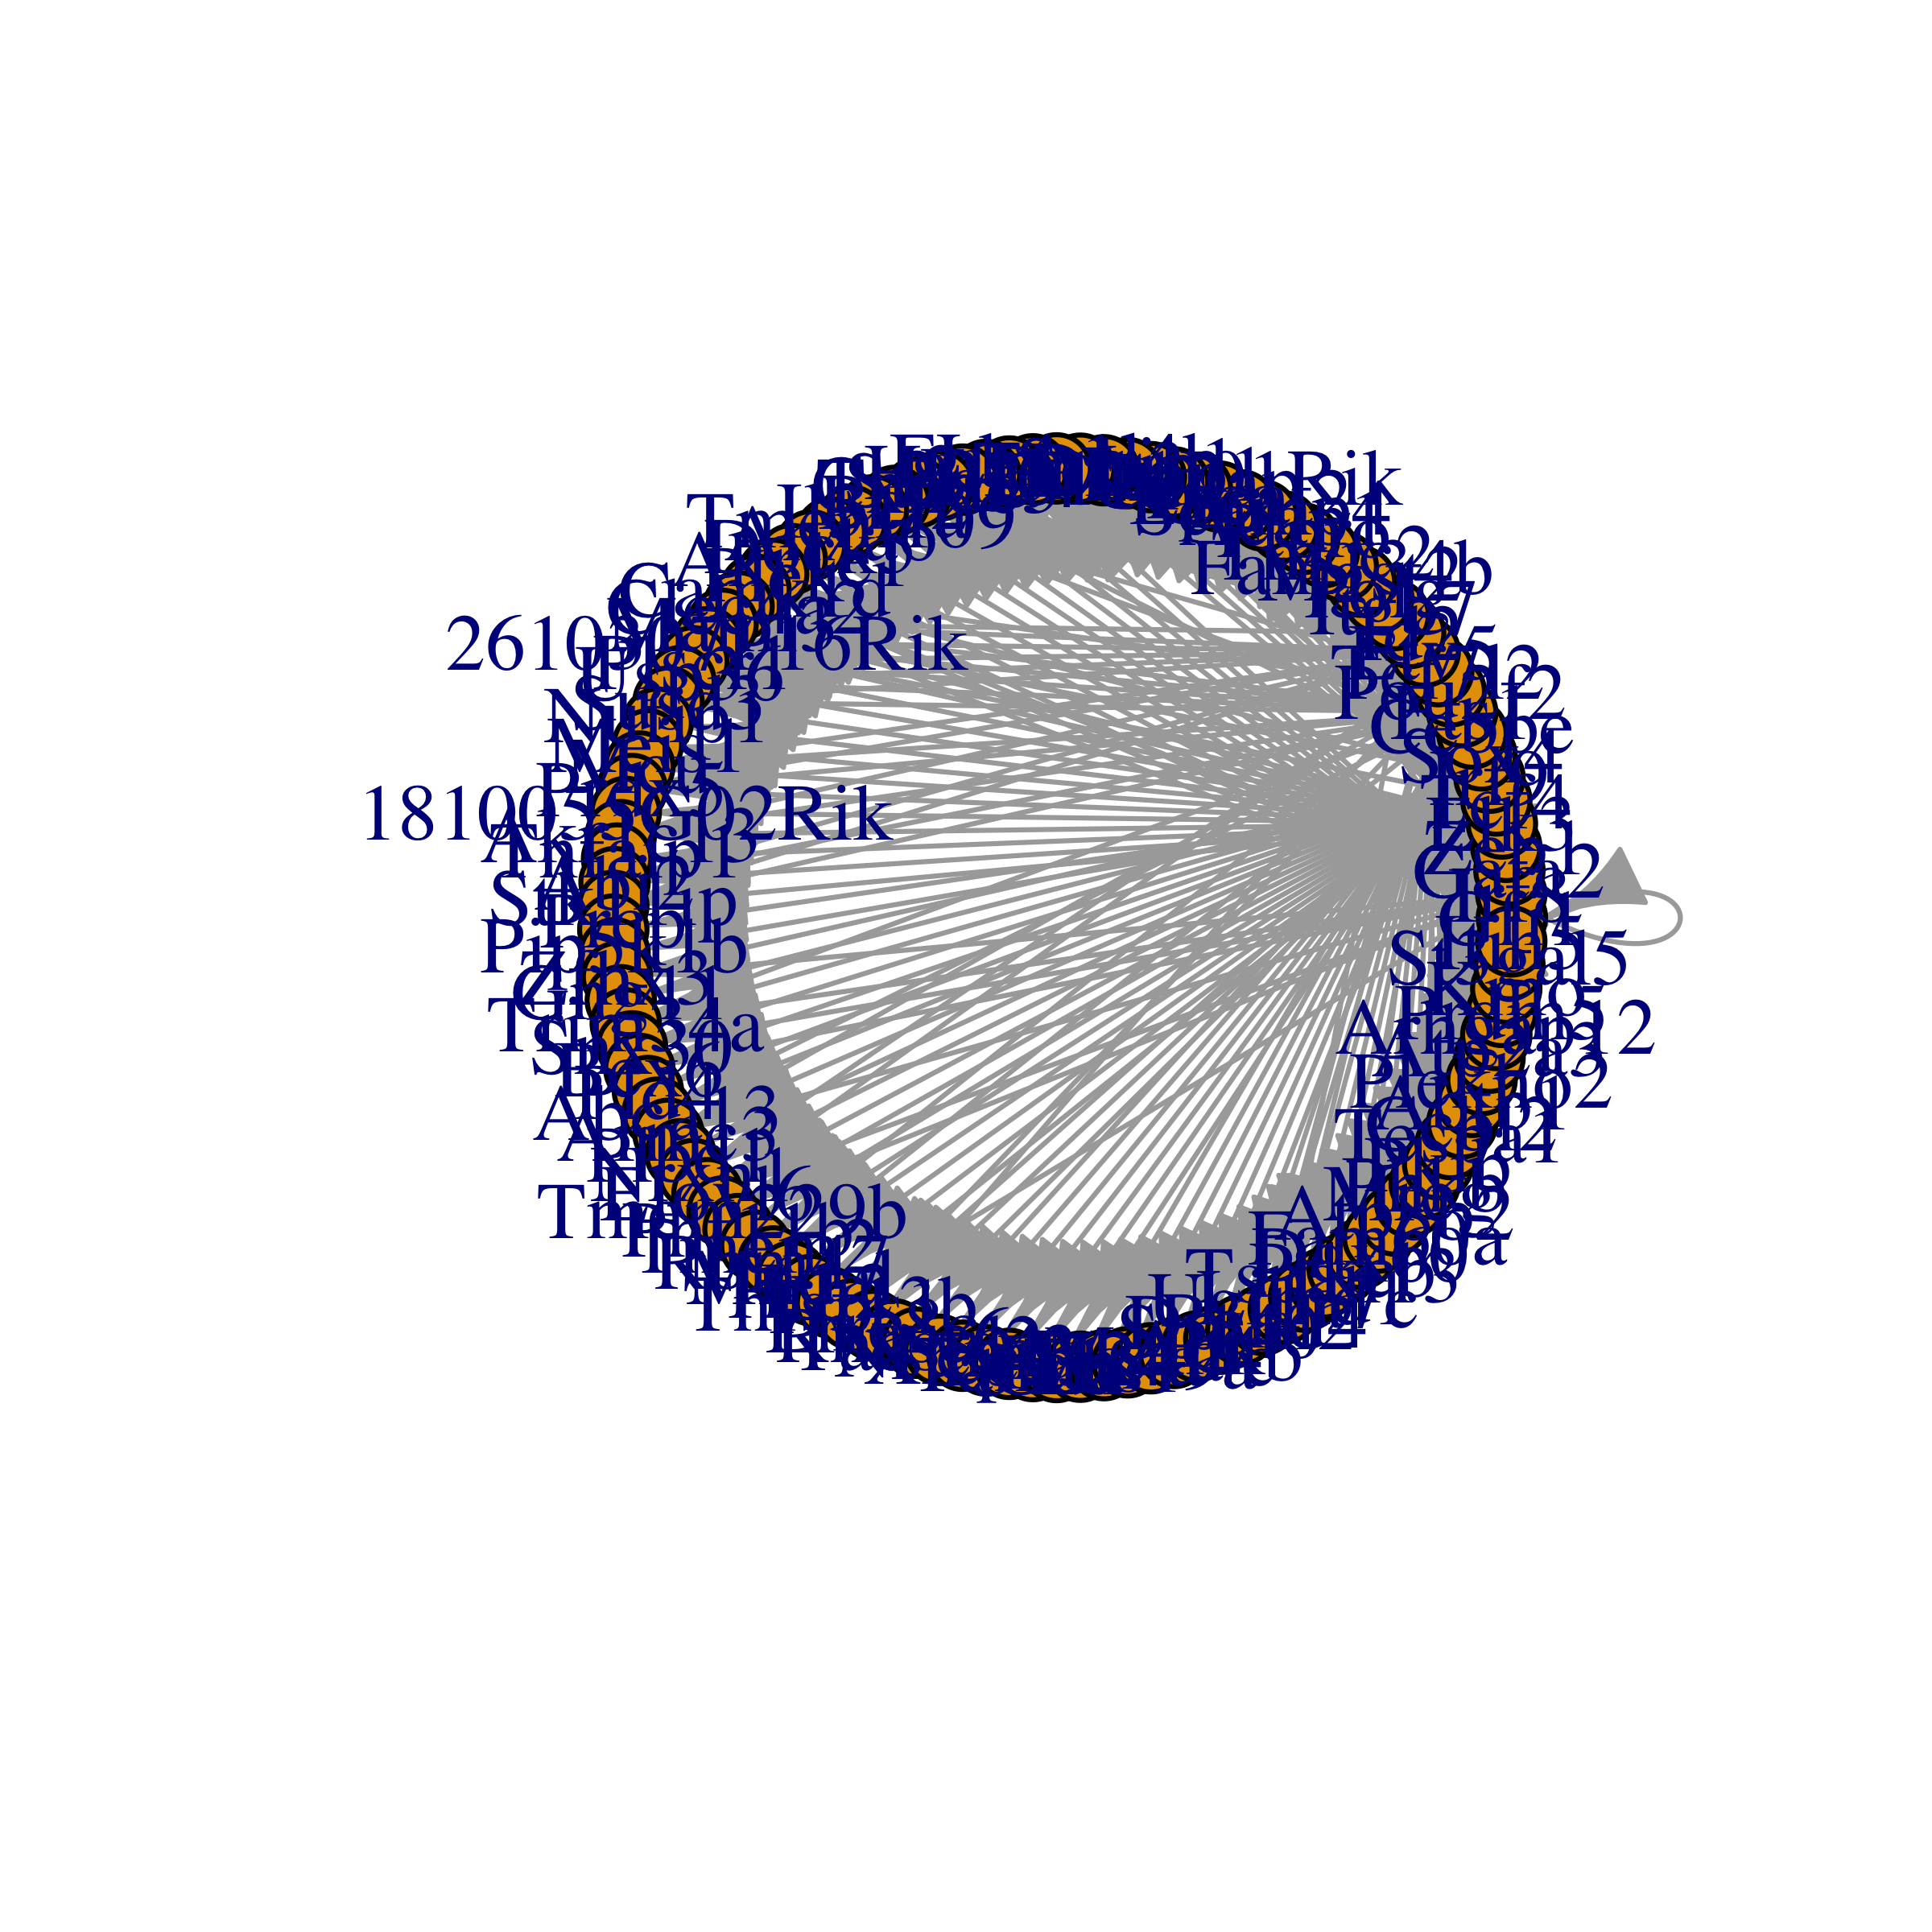
\includegraphics[width=\maxwidth]{figure/plot_network-3} 

}


\begin{kframe}\begin{alltt}
\hlcom{# plot_network(res$g, type = 'hiearchy')}
\hlkwd{plot.netbiov}\hlstd{(res)}
\end{alltt}
\end{kframe}

{\centering 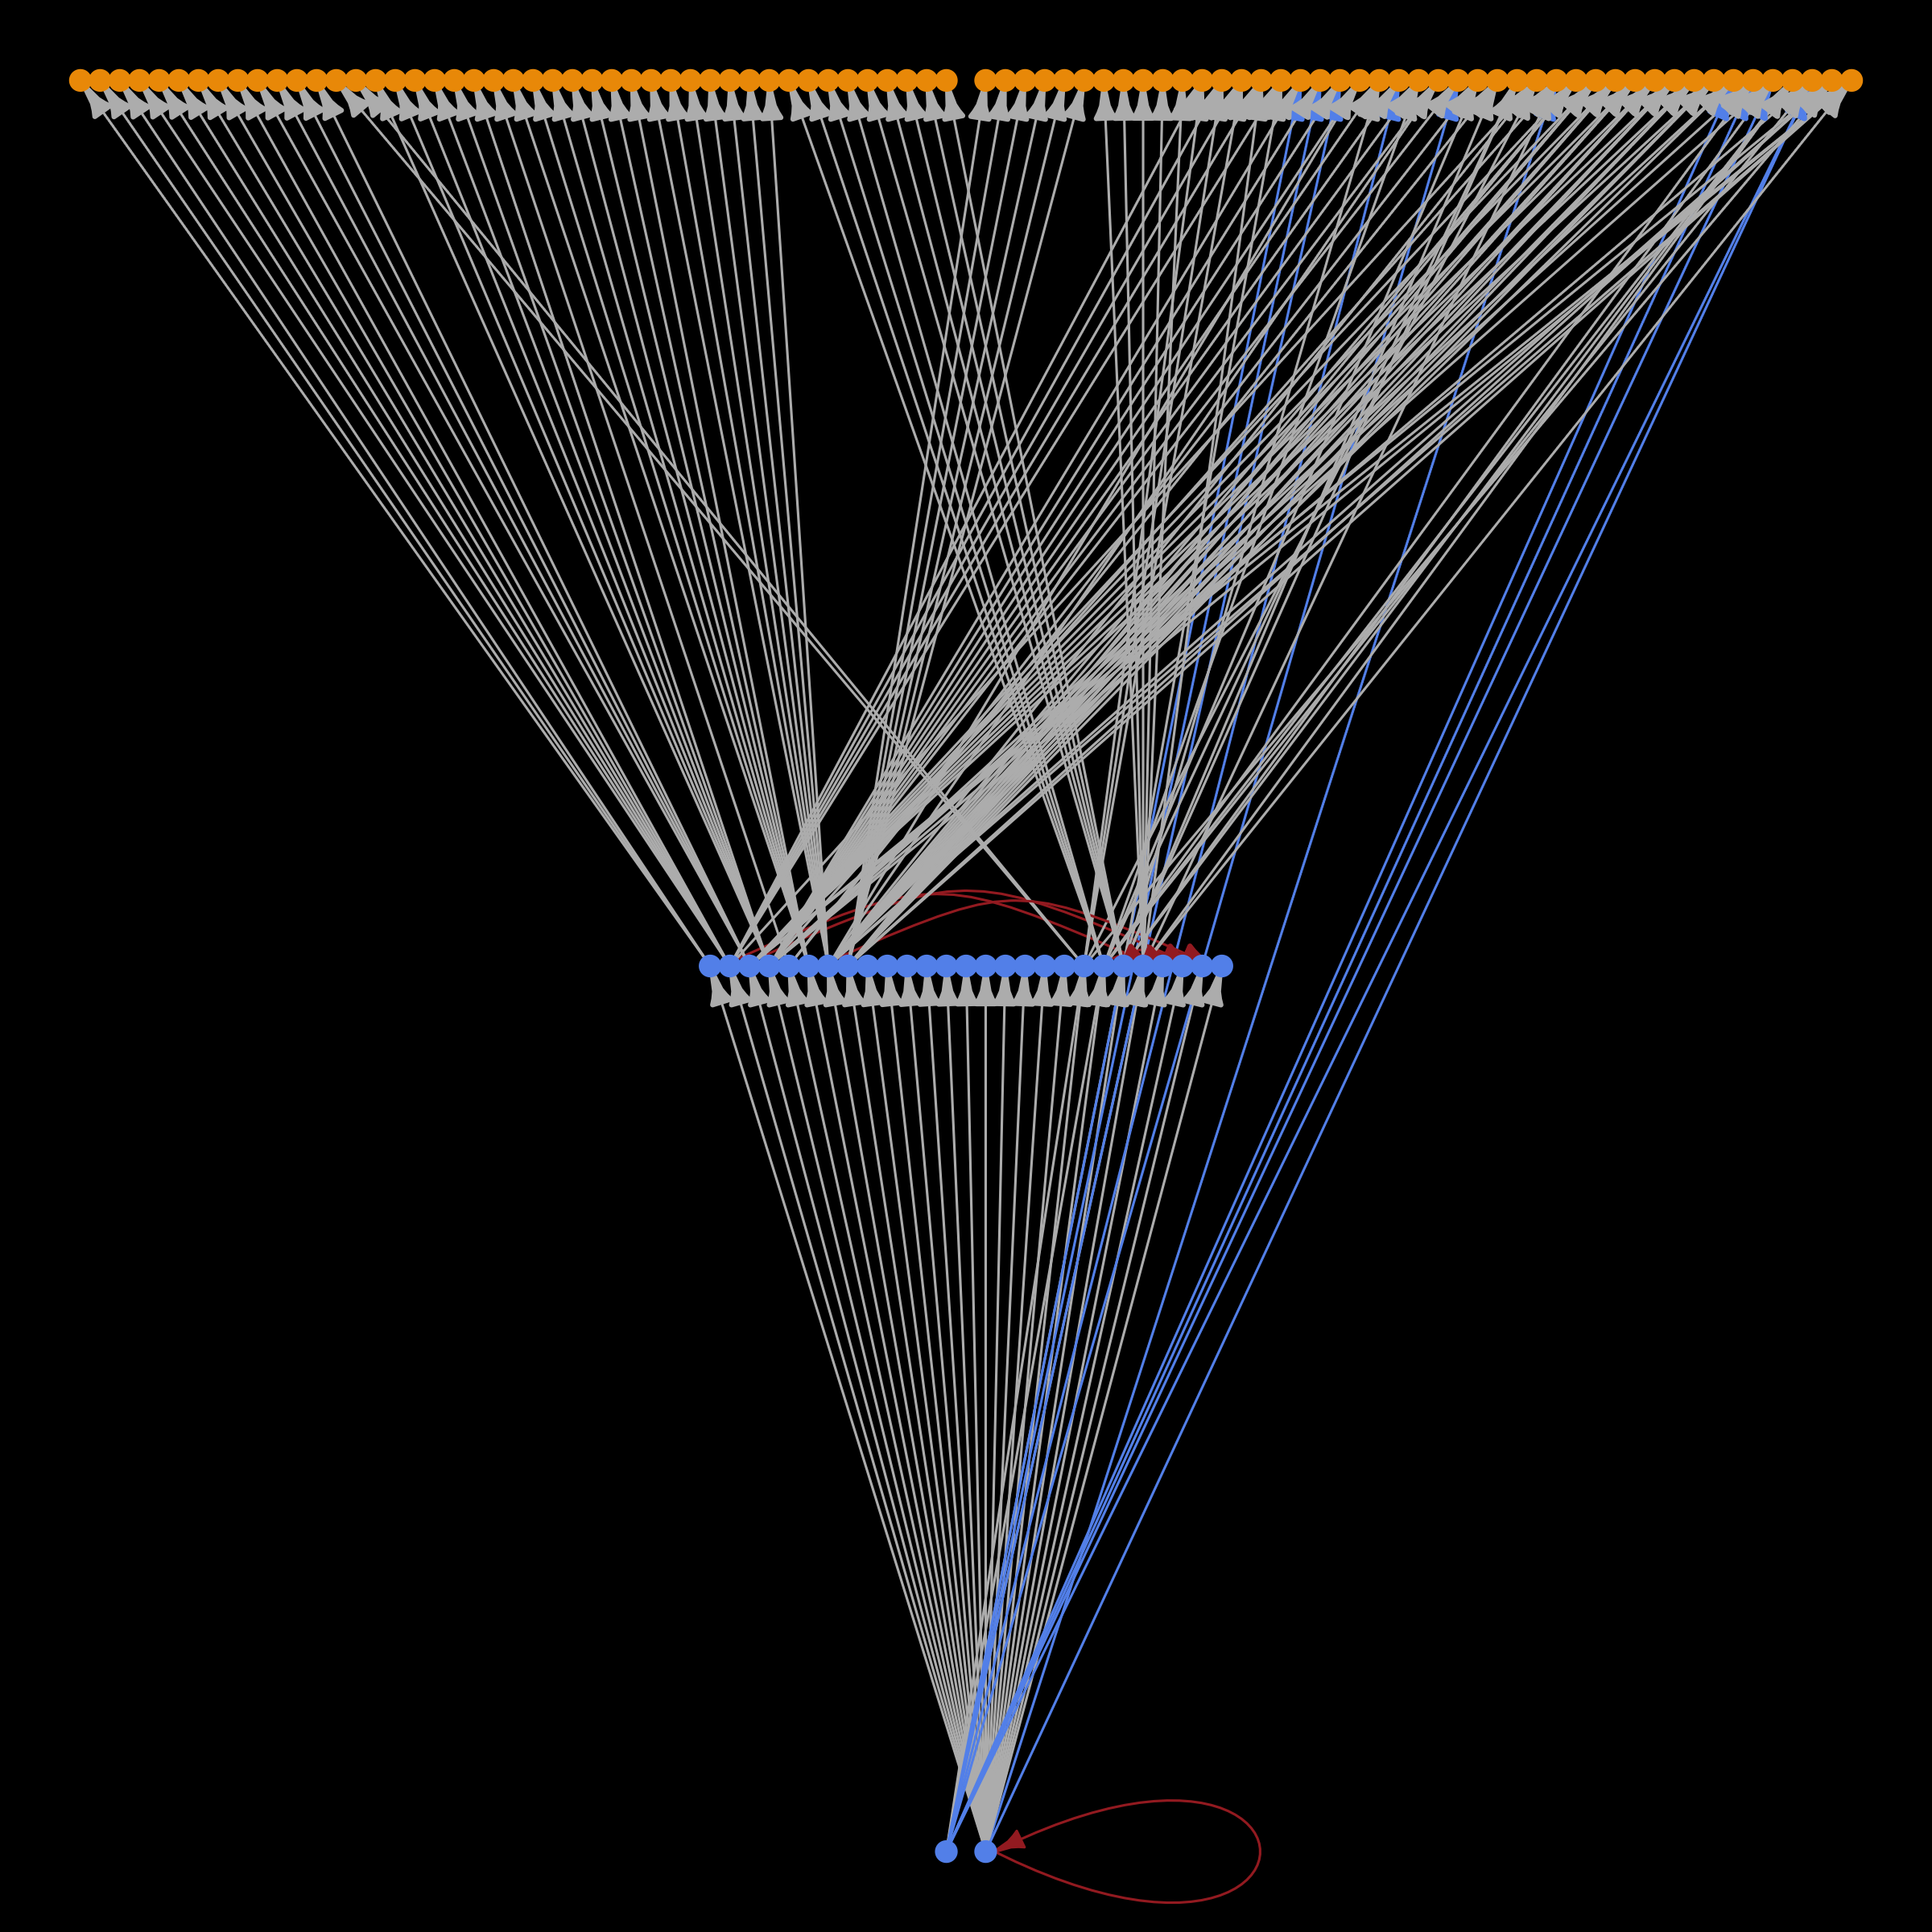
\includegraphics[width=\maxwidth]{figure/plot_network-4} 

}


\begin{kframe}\begin{alltt}
\hlkwd{plot_network}\hlstd{(res}\hlopt{$}\hlstd{g,} \hlkwc{type} \hlstd{=} \hlstr{'arcdiagram'}\hlstd{)}
\end{alltt}
\end{kframe}

{\centering 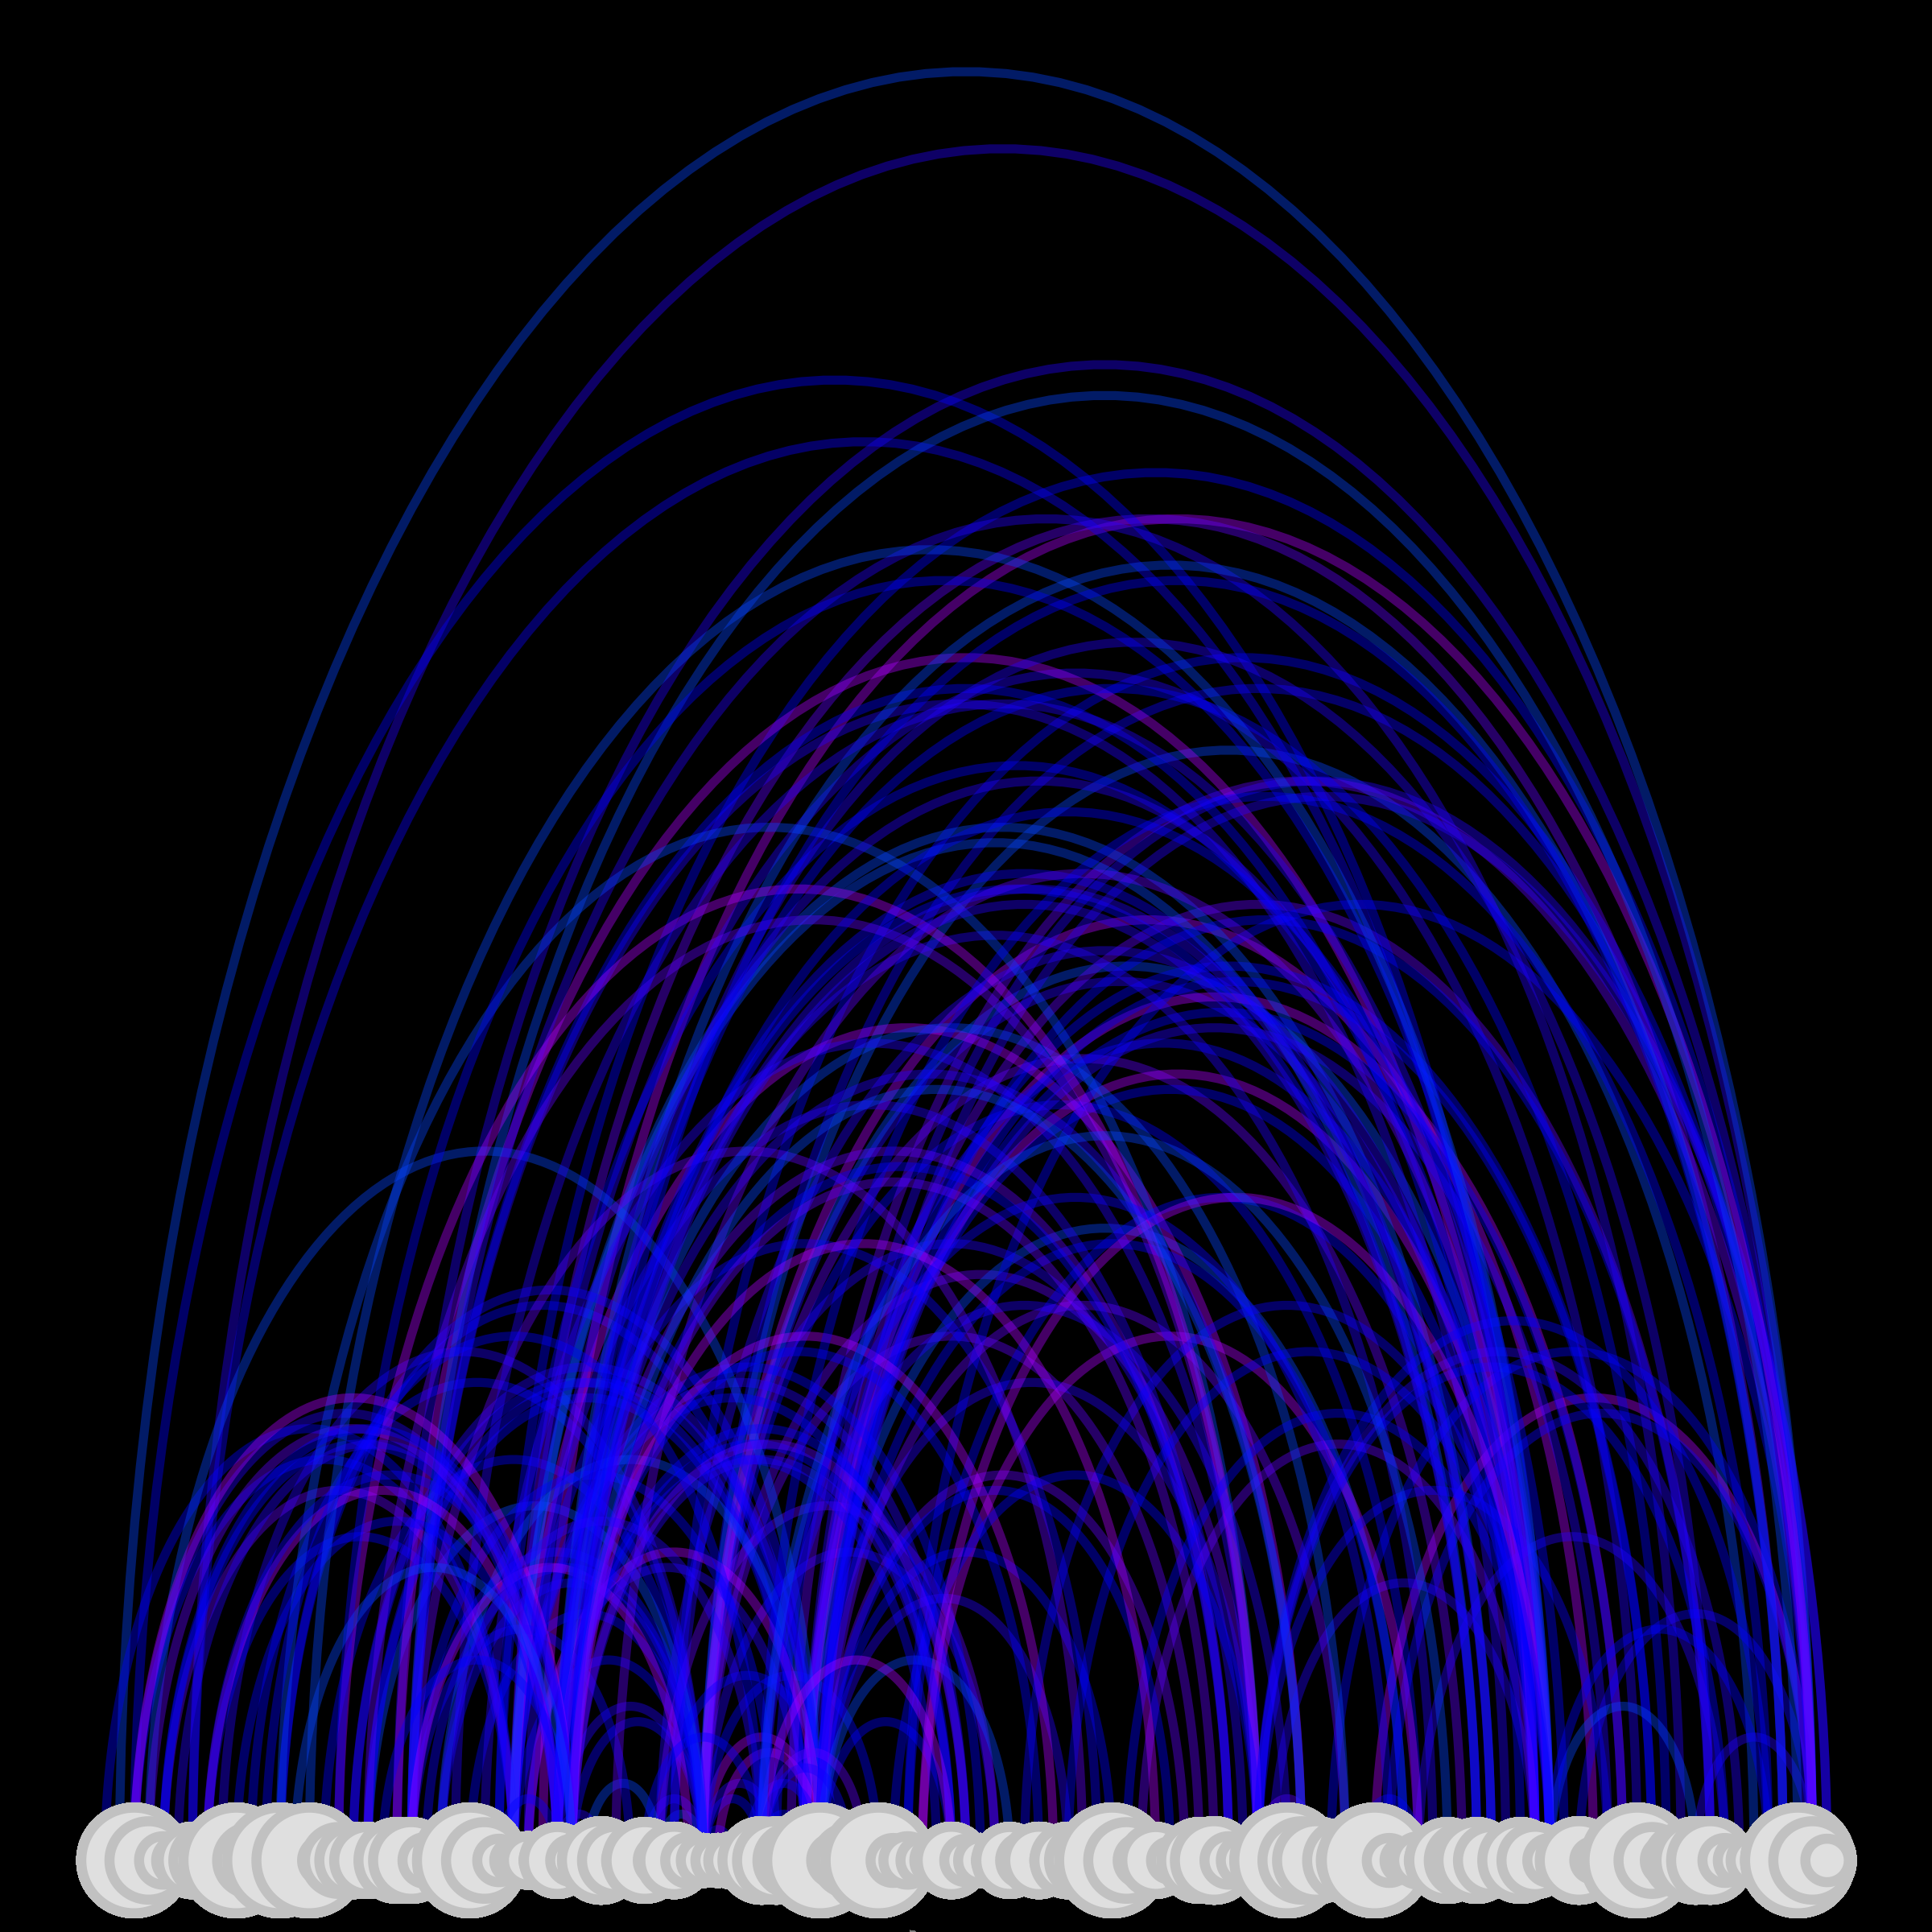
\includegraphics[width=\maxwidth]{figure/plot_network-5} 

}



\end{knitrout}

% This quick start will outline the default functions to execute in order to to analyze your data.
% If you are interested in how Monocle works and functions other than the default ones mentioned here, move onto section 3 "Getting Started with Monocle".
%
% \begin{enumerate}
% \item Store Data in a CellDataSet Object
%
% Three files are required in order to create a CellDataSet object:
%
% exprs: rows are genes and columns are cells (type = matrix)
% phenoData: rows are cells and columns are cell attributes (type = AnnotatedDataFrame)
% featureData: rows are features and columns are gene attributes (type = AnnotatedDataFrame)
%
% exprs number of columns must equal phenoData number of rows
% exprs number of rows must equal featureData number of rows
% featureData must have column named "gene\_short\_name" for certain functions
%
% Use the newCellDataSet function, as shown below, to create a new CellDataSet object with expression values measured in FPKM.  By default, Monocle assumes your data is log-normally distributed and uses a Tobit model to test for differential expression
% in downstream steps. If you are not using TPM or FPKM data go to section 2.2 on how to model it for further steps.
%
% <<quick_start_create_cds, eval=FALSE>>=
% pd <- new("AnnotatedDataFrame", data = HSMM_sample_sheet)
% fd <- new("AnnotatedDataFrame", data = HSMM_gene_annotation)
% HSMM <- newCellDataSet(as.matrix(HSMM_expr_matrix), phenoData = pd, featureData = fd)
%  @ %def
%
% \item Filter Low-quality Cells
%
%  The following lines are an example of how to display a table that reports how many cells express certain genes. detectGenes() takes a CellDataSet object and minimum threshold and will return the same CellDataSet object with all the genes that surpass the minimum threshold.
% <<quick_start_report_genes_detected, eval=FALSE>>=
% HSMM <- detectGenes(HSMM, min_expr = 0.1)
% print(head(fData(HSMM)))
% @ %def
%
% The expressed\_genes vector will hold the identifiers for genes expressed in at least 50 cells of the
% CellDataSet. This will be used later when we place cells in order of biological process.
% <<quick_start_store_expressed_genes, eval=FALSE>>=
% expressed_genes <- row.names(subset(fData(HSMM), num_cells_expressed >= 50))
% @ %def
%
% The following lines will remove cells with very low mRNA recovery or far more recovery than that of the typical cell.
% <<quick_start_filter_cells, eval=FALSE>>=
% HSMM <- HSMM[,pData(HSMM)$Total_mRNAs < 1e6]
% upper_bound <- 10^(mean(log10(pData(HSMM)$Total_mRNAs)) + 2*sd(log10(pData(HSMM)$Total_mRNAs)))
% lower_bound <- 10^(mean(log10(pData(HSMM)$Total_mRNAs)) - 2*sd(log10(pData(HSMM)$Total_mRNAs)))
% HSMM <- HSMM[,pData(HSMM)$Total_mRNAs > lower_bound & pData(HSMM)$Total_mRNAs < upper_bound]
% @ %def
%
% \item Classify Cells with CellTypeHierarchy
%
% Monocle allows you to tag different cells based on the expression of marker genes of your choosing through CellTypeHierarchies. First, create a new CellTypeHierarchy with the newCellTypeHierarchy() function. Then you can add new cell types to the CellTypeHierarchy by using the addCellType() function as shown below. The addCellType() function takes the CellTypeHierarchy you are adding the cell type to, the name of the new cell type as a string, and a classifaction function, called classify\_func, that accept expression data of each cell as input and return a boolean indicating whether or not the inputted cell is of that type.
%
% <<quick_start_set_up_cth, eval=FALSE>>=
% cth <- newCellTypeHierarchy()
%
% MYF5_id <- row.names(subset(fData(HSMM), gene_short_name == "MYF5"))
% ANPEP_id <- row.names(subset(fData(HSMM), gene_short_name == "ANPEP"))
%
% cth <- addCellType(cth, "Myoblast", classify_func = function(x) {x[MYF5_id,] >= 1})
% cth <- addCellType(cth, "Fibroblast",
%                    classify_func = function(x) {x[MYF5_id,] < 1 & x[ANPEP_id,] > 1} )
%
% HSMM <- classifyCells(HSMM, cth, 0.1)
% @ %def
%
% \item Cluster Cells with Known Marker Genes
%
% For this quick start we will be clustering cells using predetermined markers, however Monocle is capable of unsupervised cell clustering, but that is beyond the default settings that are displayed in this quick start.
%
% The markerDiffTable function accepts a CellDataSet and a CellTypeHierarchy as input and classifies all the cells in the CellDataSet into types in the CellTypeHierarchy.
% <<quick_start_cell_clustering, eval = FALSE>>=
% marker_diff <- markerDiffTable(HSMM[expressed_genes,],
%                                cth,
%                                residualModelFormulaStr = "~Media",
%                                cores = detectCores())
% @ %def
%
% <<include=FALSE, eval=TRUE>>=
% set.seed(0)
% @ %def
%
% We then assign all the genes with a q-value below 0.05 to a variable and calculate the "specifity" of those
% genes to cell type listed in the CellTypeHierarchy. The "specificity" can range from 0 to 1, the closer it is to 1 the more restricted it is to the type in question. Afterwards, selectTopMarkers will return a data table
% of the genes with the highest specificity which you can then use to determine which genes you will use for clustering. It's often best to choose the top 10 to 20 genes that are the most specific for each cell type for clustering.
% <<quick_start_cell_clustering_candidate, eval = FALSE>>=
% candidate_clustering_genes <- row.names(subset(marker_diff, qval < 0.05))
% marker_spec <- calculateMarkerSpecificity(HSMM[candidate_clustering_genes,], cth)
% head(selectTopMarkers(marker_spec, 10))
% @ %def
%
% To cluster the cells we'll choose the top ten markers for each of the cell types. An example of the procedure of clusteringCells is shown below. The parameter of clusterCells(), residualModelFormulaStr, is a model formula that identifies the effects to subtract from the   data before clustering.
% <<quick_start_cluster_cells, eval = FALSE>>=
% semisup_clustering_genes <- unique(selectTopMarkers(marker_spec, 20)$gene_id)
% HSMM <- setOrderingFilter(HSMM, semisup_clustering_genes)
% HSMM <- clusterCells(HSMM,
%                      num_clusters = 2,
%                      clustering_genes = semisup_clustering_genes,
%                      residualModelFormulaStr = "~Media + num_genes_expressed")
% @ %def
% \item Semi-Supervised Ordering with Known Marker Genes
%
% To order cells in a semi-supervised manner, first, define genes that mark progress using a new
% CellTypeHierarchy, much like we did for cell classifacation.
% <<quick_start_cell_ordering_def_genes, eval = FALSE>>=
% HSMM_myo <- HSMM[,pData(HSMM)$CellType == "Myoblast"]
%
% CCNB2_id <- row.names(subset(fData(HSMM_myo), gene_short_name == "CCNB2"))
% MYH3_id <- row.names(subset(fData(HSMM_myo), gene_short_name == "MYH3"))
%
% @ %def
%
% Then select ordering genes that co-vary with these markers.
% <<quick_start_cell_ordering_select_ordering_genes, eval = FALSE>>=
%
% cth <- newCellTypeHierarchy()
% cth <- addCellType(cth, "Cycling myoblast", classify_func = function(x) {x[CCNB2_id,] >= 1})
% cth <- addCellType(cth, "Myotube", classify_func = function(x) {x[MYH3_id,] >= 1})
%
% @ %def
%
% Finally, order the cells based on these genes.
% <<quick_start_cell_ordering_order_cells, eval = FALSE>>=
% marker_diff <- markerDiffTable(HSMM_myo[expressed_genes,],
%                                cth,
%                                cores = detectCores())
% semisup_clustering_genes <- row.names(subset(marker_diff, qval < 0.01))
% HSMM_myo <- setOrderingFilter(HSMM_myo, semisup_clustering_genes)
% @ %def
%
% <<include=FALSE, eval=TRUE>>=
% set.seed(0)
% @ %def
%
% \item Reduce Dimensionality of Data
%
% <<quick_start_reduce_dimensionality, eval = FALSE>>=
% HSMM_myo <- reduceDimension(HSMM_myo, max_components = 2)
% @ %def
%
% \item Order Cells in Pseudotime
%
% <<quick_start_order_cells, eval = FALSE>>=
% HSMM_myo <- orderCells(HSMM_myo, reverse = FALSE)
% @ %def
%
% \item Plot Genes in Pseudotime
% The first three lines are used to filter through the data so that only pseudotime is plotted for desired
% genes. The last line with the function "plot\_genes\_in\_pseudotime()" will actually plot the genes.
% <<quick_start_plot_genes_in_pseudotime, eval = FALSE>>=
% HSMM_filtered <- HSMM_myo[expressed_genes,]
% my_genes <- row.names(subset(fData(HSMM_filtered),
%                              gene_short_name %in% c("CDK1", "MEF2C", "MYOG")))
% cds_subset <- HSMM_filtered[my_genes,]
% plot_genes_in_pseudotime(cds_subset, color_by = "Hours")
% @ %def
%
% \item Determine Root of Branched Trajectory
% Monocle cannot tell which side of the cell trajectory is the beginning, however it contains methods for each scenario to make sure that the trajectory is lined up correctly with the axis.
%
% If the trajectory DOES NOT contain multiple outcomes, this is easily solved by re-ordering the cells and setting the "reverse" parameter in the orderCells() function to TRUE as the example below demonstrates
% <<quick_start_reverse_order_trajectory, eval = FALSE>>=
% HSMM_myo <- orderCells(HSMM_myo, reverse = TRUE)
% @ %def
%
% If the trajectory DOES contain multiple outcomes you can check to see if Monocle chose the correct branch as the start by generating two cell trajectories, one that colors by time and the other by pseudotime. If the branch that contains time 0, in the cell trajectory colored by time, is in the same position as the the branch that contains pseudotime 0, in the cell trajectory colored by pseudotime, then Monocle chose the correct starting point. Otherwise you will have to manually change it.
% <<quick_start_find_root, eval = FALSE>>=
% lung <- load_lung()
%
% plot_cell_trajectory(lung, color_by = "Time")
% plot_cell_trajectory(lung, color_by = "Pseudotime")
% @ %def
%
% In order to change the root we must first call plot trajectory coloring the cells by "State" to see what our options are for where we can set the root. State is Monocle's jargon for different portions of the tree. When this plot is created it will assign each branch a number
% <<quick_start_change_root_locate_opts, eval = FALSE>>=
% plot_cell_trajectory(lung, color_by = "State")
% @ %def
%
% When you have determined which branch to set as the root, call orderCells() again and set the "root\_state" parameter as the number associated with the branch you want as the root.
% <<quick_start_change_root_make_change, eval = FALSE>>=
% lung <- orderCells(lung, root_state = 3)
% @ %def
%
% \item Basic Differential Analysis
% In the myoblast data, the cells in the beginning of the experiment were cultured in "growth medium" to prevent differentiation and later switched to "differentiation medium" to promote it. The following example describes how to show which genes are affected by the switch.
% <<quick_start_basic_diff_analysis_table, eval = FALSE>>=
% diff_test_res <- differentialGeneTest(HSMM_myo, fullModelFormulaStr = "~Media")
% sig_genes <- subset(diff_test_res, qval < 0.1)
% sig_genes[, c("gene_short_name", "pval", "qval")]
% @ %def
%
% Monocle also has tools that allow you to display your data with graphs to emphasize the differences revealed by the tests above. One type of plot is the "jitter" plot as shown in the below example.
% <<quick_start_basic_diff_analysis_jitter, eval = FALSE>>=
% MYOG_ID1 <- HSMM_myo[row.names(subset(fData(HSMM_myo),
%                                       gene_short_name %in% c("MYOG", "CCNB2"))),]
% plot_genes_jitter(MYOG_ID1, grouping = "Media", ncol = 2)
% @ %def
%
% \item Find Genes that Distinguish Cell Type or State
% To test the effects of CellType on gene expression, call differentialGeneTest() on the selected genes. In order to do so you must specify a model formula, a parameter of diff\_test\_res, that indicates we are looking for genes with expression levels that depend on CellType. We do not need to specify the reduced model because
% the default value, 1, is what we want here.
% <<quick_start_find_genes_ID_cell_type, eval = FALSE>>=
% to_be_tested <- row.names(subset(fData(HSMM),
%                                  gene_short_name %in% c("UBC", "NCAM1", "ANPEP")))
% cds_subset <- HSMM[to_be_tested,]
% diff_test_res <- differentialGeneTest(cds_subset, fullModelFormulaStr = "~CellType")
% diff_test_res[,c("gene_short_name", "pval", "qval")]
%
% @ %def
%
% In order to see which genes are myoblast-specific we can again use a jitter plot to see.
% <<quick_start_find_genes_ID_graph, eval = FALSE>>=
%
% plot_genes_jitter(cds_subset, grouping = "~CellType",
%                   nrow = 1, ncol = NULL, plot_trend = TRUE)
% @ %def
%
% \item Find Genes That Are a Function of Pseudotime
% Once Monocle is able to put cells in order of a biological process, you can analyze the cells to find genes that change as the cells make progress.
% <<quick_start_find_genes_change_in_pseudotime_pick_genes, eval = FALSE>>=
% to_be_tested <- row.names(subset(fData(HSMM),
%                                  gene_short_name %in% c("MYH3", "MEF2C", "CCNB2", "TNNT1")))
% cds_subset <- HSMM[to_be_tested,]
% @ % def
%
% We need to specify a model for differential analysis that indicates change across Pseudotime as the first line
% below shows. The sm.ns in the model below indicates that Monocle should fit a natural spline through the expression values.
% <<quick_start_find_genes_change_in_pseudotime_diff_analysis, eval = FALSE>>=
% diff_test_res <- differentialGeneTest(cds_subset, fullModelFormulaStr = "~sm.ns(Pseudotime)")
% diff_test_res[,c("gene_short_name", "pval", "qval")]
% @ %def
%
% We can plot the expression levels of these genes with the plot\_genes\_in\_pseudotime() function.
% <<quick_start_find_genes_change_in_pseudotime_graph, eval = FALSE>>=
% plot_genes_in_pseudotime(cds_subset, color_by = "Hours")
% @ %def
%
% \item Analyzing Branches in Single-Cell Trajectories
%
% Monocle contains several tools for analyzing the branching events of trajectories with multiple outcomes.
% To analyze how genes are expressed differently in a branch compared to its root, Monocle incorporates branched expression analysis modeling, or BEAM. BEAM takes a CellDataSet ordered by orderCells and the name of a branch point in the trajectory and returns a table of significance scores for each gene. Genes that score significant are branch-dependent in their expression.
% <<quick_start_perform_BEAM, eval = FALSE>>=
% lung <- load_lung()
% BEAM_res <- BEAM(lung, branch_point = 1, cores = detectCores())
% BEAM_res <- BEAM_res[order(BEAM_res$qval),]
% BEAM_res <- BEAM_res[,c("gene_short_name", "pval", "qval")]
% @ %def
%
% <<include=FALSE, eval=TRUE>>=
% set.seed(0)
% @ %def
%
% You can visualize changes for all genes that are significantly branch-dependent with a special type of
% heatmap. This heatmap will show both lineages simultaneously. This heatmap requires you to enter a specifc branch point. The start of the branch point is represented by the middle of the heatmap, going from the middle to the left is one branch and going from the middle to the right is the other branch.
% <<quick_start_analyze_branches_single_cell_trajectory_heat, eval = FALSE>>=
% plot_genes_branched_heatmap(lung[row.names(subset(BEAM_res, qval < 1e-4)),],
%                             branch_point = 1,
%                             num_clusters = 4,
%                             cores = detectCores(),
%                             use_gene_short_name = T,
%                             show_rownames = T)
% @ %def
%
% <<include=FALSE, eval=TRUE>>=
% set.seed(0)
% @ %def
%
% We can also plot these genes in pseudotime using plot\_genes\_branched\_pseudotime() which is quite similar to plot\_genes\_in\_pseudotime except that shows two kinetic trends, one for each lineage, instead of one.
% <<quick_start_analayze_branches_single_cell_trajectory_heat, eval = FALSE>>=
% lung_genes <- row.names(subset(fData(lung), gene_short_name %in% c("Ccnd2", "Sftpb", "Pdpn")))
% plot_genes_branched_pseudotime(lung[lung_genes,],
%                                branch_point = 1,
%                                color_by = "Time",
%                                ncol = 1)
% @ %def
%

 \section{The Scribe object}

 The \Rpackage{monocle} package takes a matrix of gene expression values as calculated by Cufflinks\cite{Trapnell:2012kp} or another gene expression estimation program. Monocle can work with relative expression values (e.g. FPKM or TPM units) or absolute transcript counts (e.g. from UMI experiments). Monocle also works ``out-of-the-box'' with the transcript count matrices produced by \href{https://support.10xgenomics.com/single-cell/software/overview/welcome}{CellRanger}, the software pipeline for analyzing experiments from the 10X Genomics Chromium instrument. Monocle also works well with data from other RNA-Seq workflows such as \href{http://biorxiv.org/content/early/2017/02/02/104844}{sci-RNA-Seq} and instruments like the Biorad ddSEQ. Although Monocle can be used with raw read counts, these are not directly proportional to expression values unless you normalize them by length, so some Monocle functions could produce nonsense results. If you don't have UMI counts, We recommend you load up FPKM or TPM values instead of raw read counts.

 \subsection{The Scribe class: need to discuss}

 \Rpackage{Scribe} holds single cell expression data in objects of the \Rclass{CellDataSet} class. The class is derived from the Bioconductor \Rclass{ExpressionSet} class, which provides a common interface familiar to those who have analyzed microarray experiments with Bioconductor. The class requires three input files:
 \begin{enumerate}
 \item \Robject{exprs}, a numeric matrix of expression values, where rows are genes, and columns are cells
 \item \Robject{phenoData}, an \Rpackage{AnnotatedDataFrame} object, where rows are cells, and columns are cell attributes (such as cell type, culture condition, day captured, etc.)
 \item \Robject{featureData}, an \Rpackage{AnnotatedDataFrame} object, where rows are features (e.g. genes), and columns are gene attributes, such as biotype, gc content, etc.
 \end{enumerate}

 The expression value matrix \emph{must} have the same number of columns as the \Robject{phenoData} has rows, and it must have the same number of rows as the \Robject{featureData} data frame has rows. Row names of the \Robject{phenoData} object should match the column names of the expression matrix. Row names of the \Robject{featureData} object should match row names of the expression matrix. Also, one of the columns of the
 \Robject{featureData} must be named "gene\_short\_name".

 You can create a new \Rclass{CellDataSet} object as follows:

This will create a CellDataSet object with expression values measured in FPKM, a measure of relative expression reported by Cufflinks. By default, Monocle assumes that your expression data is in units of transcript counts and uses a negative binomial model to test for differential expression in downstream steps. However, if you're using relative expression values such as TPM or FPKM data, see below for how to tell Monocle how to model it in downstream steps.

\textbf{NOTE:} if you do have UMI data, you should \emph{not} normalize it yourself prior to creating your \Robject{CellDataSet}. You should also \emph{not} try to convert the UMI counts to relative abundances (by converting it to FPKM/TPM data). You should \emph{not} use \Rfunction{relative2abs()} as discussed below in section \ref{conv_rel2abs}. Monocle will do all needed normalization steps internally. Normalizing it yourself risks breaking some of Monocle's key steps.

 %\section{Tips and tricks}

\section{Relationship between Scribe and Monocle 2 as well as other relevant packages}
\Rpackage{Scribe} relies on \Rpackage{Monocle 2} for reconstructing the single-cell trajectory before inferring causal network. We extended \Rpackage{Monocle 2} in a few aspects to account for the specific requirement for \Rpackage{Scribe}. For example, in order to avoid the over-crowded nature of the cells at the terminal regions of the trajectory, we applied a simple strategy to first run Monocle 2 using DDRTree to get the trajectory with complex branches and then reorder the trajectory for each branch (from the source state to the terminal state) using principal curve (simplePPT) with the low dimension space obtained from the diffusion map dimension reduction technique. \Rpackage{Scribe} provides various methods for infering the regulatory relationship, mutual information, Granger causality and CCM. We used the implementation from parmigene, vars and rEDM respectively. To intuitively visualize the casual regulation between pairs of genes, we generalized the DREVI approach (\cite{}). The network visualization relies on the igraph, netbiov, arcdiagram as well as the HiveR packages.

We are preparing a manuscript describing \Rpackage{Scribe} for reconstructing causal regulatory network.

\section{Theory behind Scribe}\label{theory}

\subsection{Restricted direct information}\label{RDI}
A very well-known measure of interdependence of two random variables $X$ and $Y$ was first proposed by [cite] called mutual information, is defined as:
\begin{equation}
I(X;Y)=\sum_{x,y} p_{XY}(x,y) \log\frac{p_{XY}(x,y)}{p_X(x)p_Y(y)}
\end{equation}

The mutual information between $X$ and $Y$is equal to zero if and only if $X$ and $Y$ are independent. The mutual information of two variables given a third random variable $Z$ is defined as:

\begin{equation}
I(X;Y|Z)=\sum_{x,y,z} p_{XYZ}(x,y,z) \log\frac{p_{XY|Z}(x,y|z)}{p_{X|Z}(x|z)p_{Y|Z}(y|z)}
\end{equation}

Similarly, the mutual information between $X$ and $Y$ given $Z$ is equal to zero if and only if $X$ and $Y$ are independent given $Z$.
In general, $X$, $Y$ and $Z$ can be multi-dimensional random variables with arbitrary dimensions, such as in the case that the variables are time-series $\underline{X}^t$, $\underline{Y}^t$ and $\underline{Z}^t$. So the mutual information between the time-series can be defined similarly as $ I(\underline{X}^t,\underline{Y}^t,\underline{Z}^t) $.
Now the question we might ask ourselves is is it possible to define a measure for the amount of information the past state(s) of $X$ provide about the current state of the variable $Z$ denoted by $Z(t-1)$? [cite: DI paper] provides such a measure called Directed Information, sometimes referred to as "Transfer Entropy" [cite: T. Schreiber, Measuring information transfer," Physical review letters, vol. 85, no. 2, p. 461, 2000]. The directed information from the time-series $\underline{X}^T$ to $\underline{Y}^T$ is defined as:

\begin{equation}
DI(X\rightarrow Y)=\sum_{t=1}^T I(\underline{X}^{t-1}; Y(t)|\underline{Y}^{t-1})
\end{equation}


The conditioned version of it also can be defined similarly:

\begin{equation}
DI(X\rightarrow Y|Z)=\sum_{t=1}^T I(\underline{X}^{t-11}; Y(t)|\underline{Y}^{t-1},\underline{Z}^{t-1})
\end{equation}

(Mention the theorem for DI) [Cite DI paper]

In [Cite DI paper] it is shown that if the system is not purely deterministic, then the directed information graph (DIG) and the causality graph (CG) are identical. However, they have shown that if the relationship in the dynamic system is purely deterministic, then the algorithm is unable to return the correct causality graph. It is contrary to CCM method which only deals with the deterministic systems and is unable to perceive the graph in a stochastic (noisy) system.
Thus in the case of the first-order Markov systems we introduce an alternate version of DI which employs only the immediate past of the system instead of the whole past samples:

\begin{equation}
DI(X\rightarrow Y)= I \left( X(t-1); Y(t)|Y(t-1) \right)
\end{equation}

and the conditioned version of it can be expressed as:

\begin{equation}
DI(X\rightarrow Y|Z)= I \left( X(t-1); Y(t)|Y(t-1),Z(t-1) \right)
\end{equation}

In [Cite: Our Allerton paper] it's shown that this method works in many stochastic or deterministic cases and under some mild assumptions it's capable of inferring the correct graph.

\subsection{Network sparsifier}
%
% \section{Using Monocle with other data types}
%
% This section is yet to be written.

 \section{Citation}\ref{citations}
 If you use \Rpackage{Scribe} to analyze your experiments, please cite:
\begin{knitrout}
\definecolor{shadecolor}{rgb}{0.969, 0.969, 0.969}\color{fgcolor}\begin{kframe}
\begin{alltt}
\hlkwd{citation}\hlstd{(}\hlstr{"Scribe"}\hlstd{)}
\end{alltt}
\begin{verbatim}
## 
## To cite package 'Scribe' in publications use:
## 
##   ANN Library: David Mount, Sunil Arya. flann Packge:
##   http://www.cs.ubc.ca/research/flann/. InformationEstimator:
##   Xiaojie Qiu, Arman Rahimzamani, Sreeram Kannan and Cole Trapnell
##   (2017). Scribe: Restricted direction information for network
##   inference. R package version 0.1.
##   https://CRAN.R-project.org/package=Scribe
## 
## A BibTeX entry for LaTeX users is
## 
##   @Manual{,
##     title = {Scribe: Restricted direction information for network inference},
##     author = {ANN Library: David Mount and Sunil Arya. flann Packge: http://www.cs.ubc.ca/research/flann/. InformationEstimator: Xiaojie Qiu and Arman Rahimzamani and Sreeram Kannan and Cole Trapnell},
##     year = {2017},
##     note = {R package version 0.1},
##     url = {https://CRAN.R-project.org/package=Scribe},
##   }
## 
## ATTENTION: This citation information has been auto-generated from
## the package DESCRIPTION file and may need manual editing, see
## 'help("citation")'.
\end{verbatim}
\end{kframe}
\end{knitrout}

 \section{Acknowledgements}

Scribe was written by Xiaojie Qiu which is based on the python package originally developed by Arman Rahimzamani, with substantial design input Cole Trapnell and Sreeram Kannan. The core of Scribe on estimating restricted direction information (RDI) is written in Rcpp for speed accerlationp. We are grateful to all members from Trapnell and Kannan lab, especially XXX for technical assistance, and Andysheh Mohajeri, Jonanthan Packer, XXX etc. for helpful discussions. This work was supported by  US National Institutes of Health (NIH) grants DP2 HD088158 (C.T.) and U54 DK107979 (C.T.), XXXXXX; C.T. is partly supported by a Dale. F. Frey Award for Breakthrough Scientists and an Alfred P. Sloan Foundation Research Fellowship.

This vignette was created from Wolfgang Huber's Bioconductor vignette style document, and patterned after the vignette for \Rpackage{DESeq}, by Simon Anders and Wolfgang Huber.

\section{Session Info}
\begin{knitrout}
\definecolor{shadecolor}{rgb}{0.969, 0.969, 0.969}\color{fgcolor}\begin{kframe}
\begin{alltt}
\hlkwd{sessionInfo}\hlstd{()}
\end{alltt}
\begin{verbatim}
## R version 3.3.2 (2016-10-31)
## Platform: x86_64-apple-darwin13.4.0 (64-bit)
## Running under: OS X Yosemite 10.10.5
## 
## locale:
## [1] en_US.UTF-8/en_US.UTF-8/en_US.UTF-8/C/en_US.UTF-8/en_US.UTF-8
## 
## attached base packages:
##  [1] splines   stats4    parallel  stats     graphics  grDevices utils    
##  [8] datasets  methods   base     
## 
## other attached packages:
##  [1] plyr_1.8.4          Scribe_0.1          arcdiagram_0.1.11  
##  [4] netbiov_1.8.0       igraph_1.1.2        shiny_1.0.3        
##  [7] plotly_4.6.0        inflection_1.3      vars_1.5-2         
## [10] lmtest_0.9-35       urca_1.3-0          strucchange_1.5-1  
## [13] sandwich_2.3-4      zoo_1.8-0           MASS_7.3-47        
## [16] rEDM_0.5.4          monocle_2.5.3       DDRTree_0.1.5      
## [19] irlba_2.2.1         VGAM_1.0-3          Matrix_1.2-10      
## [22] ggplot2_2.2.1       reshape2_1.4.2      Biobase_2.34.0     
## [25] BiocGenerics_0.20.0 knitr_1.15.1       
## 
## loaded via a namespace (and not attached):
##  [1] Rcpp_0.12.12           lattice_0.20-35        tidyr_0.6.3           
##  [4] assertthat_0.2.0       digest_0.6.12          mime_0.5              
##  [7] slam_0.1-40            R6_2.2.1               qlcMatrix_0.9.5       
## [10] evaluate_0.10          httr_1.2.1             highr_0.6             
## [13] rlang_0.1.1            lazyeval_0.2.0         combinat_0.0-8        
## [16] labeling_0.3           Rtsne_0.13             stringr_1.2.0         
## [19] htmlwidgets_0.8        pheatmap_1.0.8         munsell_0.4.3         
## [22] httpuv_1.3.3           pkgconfig_2.0.1        htmltools_0.3.6       
## [25] tibble_1.3.1           xacHelper_0.0.1.0000   codetools_0.2-15      
## [28] matrixStats_0.52.2     viridisLite_0.2.0      dplyr_0.5.0           
## [31] grid_3.3.2             densityClust_0.2.1     xtable_1.8-2          
## [34] nlme_3.1-131           jsonlite_1.4           gtable_0.2.0          
## [37] DBI_0.6-1              magrittr_1.5           scales_0.4.1          
## [40] stringi_1.1.5          limma_3.30.13          fastICA_1.2-0         
## [43] RColorBrewer_1.1-2     tools_3.3.2            purrr_0.2.2.2         
## [46] HSMMSingleCell_0.108.0 colorspace_1.3-2       cluster_2.0.6
\end{verbatim}
\end{kframe}
\end{knitrout}

\bibliographystyle{unsrt}
\bibliography{Scribe_alg}

\end{document}
